\documentclass[aspectratio=169]{beamer}

\usepackage[utf8]{inputenc}
%\usepackage{emoji}

\usepackage{amsmath}
\usepackage{graphicx}
\usepackage[T1]{fontenc}
\usepackage{Oswald}
\usepackage{array}

\usepackage{enumitem}
\setitemize{label=\usebeamerfont*{itemize item}%
  \usebeamercolor[fg]{itemize item}
  \usebeamertemplate{itemize item},
}
\setbeamertemplate{itemize item}[square]
\setbeamertemplate{itemize subitem}[circle]

\usepackage{pgfplots}
\pgfplotsset{compat=1.18}
\usepackage{tikz}
\usepgfplotslibrary{fillbetween}


% \tikzset{
% 	invisible/.style={opacity=0},
% 	visible on/.style={alt={#1{}{invisible}}},
% 	alt/.code args={<#1>#2#3}{%
% 		\alt<#1>{\pgfkeysalso{#2}}{\pgfkeysalso{#3}} % \pgfkeysalso doesn't change the path
% 	},
% }

%\pgfplotsset{every axis/.append style={label style={font=\small},tick label style={font=\footnotesize} }}

\newcommand{\graphheight}{7cm}
\newcommand{\graphwidth}{11cm}

\newcommand{\E}[1]{E\left[#1 \right]}
\newcommand{\ind}[1]{\mathbf{1}_{#1}}

%\newcommand{\P}[1]{E\left[#1\right]}

% \definecolor{azulcito}{RGB}{20,70,140}
\definecolor{azulcito}{RGB}{0,80,150}
\definecolor{verdecito}{RGB}{80,150,0}
\definecolor{rojito}{RGB}{150,0,80}
\definecolor{violetita}{RGB}{150,20,150}


\setbeamercolor*{structure}{fg=azulcito,bg=azulcito!20!white}
\setbeamercolor*{alerted text}{fg=azulcito}

  \setbeamercolor{block title}{fg=azulcito,bg=azulcito!20!white}
  \setbeamercolor{block body}{fg=black,bg=azulcito!10!white}
  
\beamertemplatenavigationsymbolsempty

\setbeamercolor*{author in head/foot}{fg=azulcito,bg=azulcito!15!white}
\setbeamercolor*{title in head/foot}{fg=azulcito,bg=azulcito!15!white}
\setbeamercolor*{date in head/foot}{fg=azulcito,bg=azulcito!15!white}

% Pgfplots
\pgfplotsset{width=\graphwidth, height = \graphheight, grid style = {dashed, gray}, every tick label/.append style = {font=\footnotesize}, compat=1.18, legend style={font=\footnotesize, draw=none, fill=none}, every axis/.append style={label style={font=\footnotesize}}}

\tikzset{>=stealth}

\newtheorem{proposition}{Proposition}

\defbeamertemplate*{footline}{mitema}
{
  \leavevmode%
  \hbox{%
  \begin{beamercolorbox}[wd=.25\paperwidth,ht=2.25ex,dp=1ex,left]{author in head/foot}%
    \usebeamerfont{author in head/foot}\hspace*{2ex}\insertshortauthor
  \end{beamercolorbox}%
  \begin{beamercolorbox}[wd=.5\paperwidth,ht=2.25ex,dp=1ex,center]{title in head/foot}%
    \usebeamerfont{date in head/foot}\insertshortdate{}
  \end{beamercolorbox}%
  \begin{beamercolorbox}[wd=.25\paperwidth,ht=2.25ex,dp=1ex,right]{date in head/foot}%
    \insertframenumber{}/\inserttotalframenumber\hspace*{2em} 
  \end{beamercolorbox}}%
 \vskip0pt%
}


\setbeamercolor{blocky}{fg=azulcito,bg=azulcito!15!white}
\setbeamercolor{blocky2}{fg=black,bg=azulcito!10!white}

\defbeamertemplate*{title page}{customized}[1][]
{
{\flushright
  \begin{beamercolorbox}[wd=\paperwidth,ht=6em,dp=1ex,right,rightskip=1.5em]{blocky}%
    \usebeamerfont{title}{\huge \inserttitle}\par \vspace{.9em}
    \usebeamerfont{subtitle}{\Large \insertsubtitle}\par \vspace{.5em}
  \end{beamercolorbox}%
  \vfill
    \usebeamerfont{author}{\Large \insertauthor}\par \vspace{1em}
      \usebeamerfont{institute}{\large \insertinstitute}\par
  
  
  \vfill
  \usebeamerfont{date}{\insertdate}\par
  %\usebeamercolor[fg]{titlegraphic}\inserttitlegraphic
  }
}

\usefonttheme[onlymath]{serif}

\title{Caching and pre-fetching: the role of hazard rates.}

\author[Andres Ferragut, Universidad ORT Uruguay]{Andres Ferragut\\[.6em] \normalsize joint work with Matias Carrasco and Fernando Paganini}
\institute{Universidad ORT Uruguay}
\date[LINCS Seminar -- May 2024]{Laboratory for Information, Networking and Communication Sciences Seminar -- May 2024}

\AtBeginSection[]
{
\begin{frame}{Outline}
\tableofcontents[currentsection, 
   hideallsubsections, 
   sectionstyle=show/shaded,
]
\end{frame}
}

\newenvironment*{myitem}[1][1.5em]{\begin{itemize}\setlength{\itemsep}{#1}}{\end{itemize}}

\begin{document}

\frame[plain]{\titlepage}

\begin{frame}{Outline}
\tableofcontents
\end{frame}

\section{The caching problem}

\begin{frame}{The caching problem}
	
	\begin{columns}
		\begin{column}{0.61\textwidth}
			\begin{myitem}[2em]
				\item Consider a \alert{local memory system} that handles items from a catalog of $N$ objects.
				\item Requests for objects arrive as a random process.
				\item The memory (cache) can locally store $C<N$ of them.
				\item If item is in cache, we have a \alert{hit}. Otherwise, it is a \alert{miss}.
			\end{myitem}
		\end{column}
		\begin{column}{0.39\textwidth}
			\centering
			\resizebox{\columnwidth}{!}{
\begin{tikzpicture}
				\node (lambda) at (0,0) {$\lambda$};
				\node[draw,circle] (cache) at (2,0) {Cache};
				\node[draw,rectangle, fill=verdecito!20!white] (file1) at (5,2) {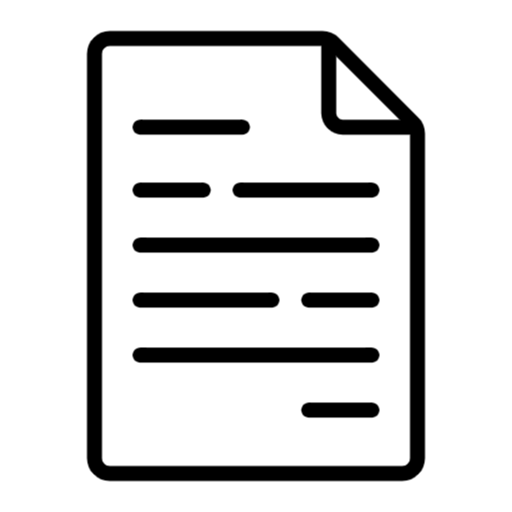
\includegraphics[width=.5cm]{figuras/file.png} File 1};
				\node[draw,rectangle,fill=rojito!20!white] (file2) at (5,1) {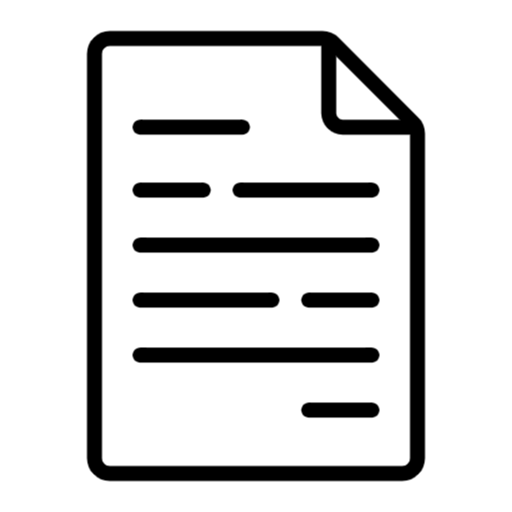
\includegraphics[width=.5cm]{figuras/file.png} File 2};
				\node[draw,rectangle, fill=verdecito!20!white] (file3) at (5,0) {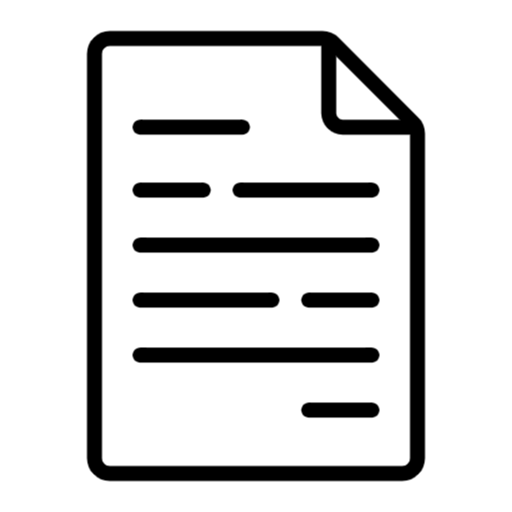
\includegraphics[width=.5cm]{figuras/file.png} File 3};
				\node (dots) at (5,-1) {$\vdots$};
				\node[draw,rectangle, fill=rojito!20!white] (fileN) at (5,-2) {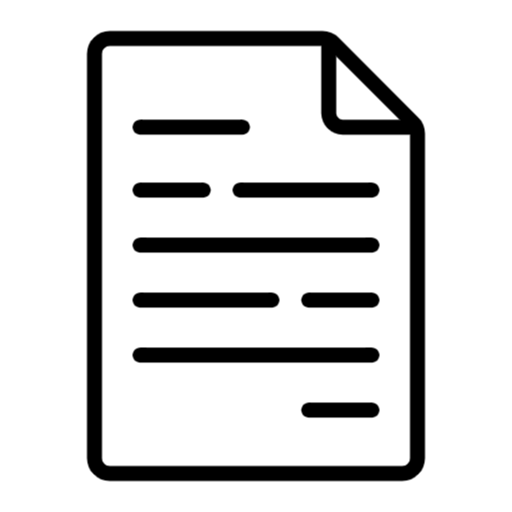
\includegraphics[width=.5cm]{figuras/file.png} File $N$};

				\draw[->,very thick, azulcito] (lambda) -- (cache);
				\draw[->,very thick, dashed, verdecito] (file1.west)--(cache);
				\draw[->,very thick, rojito] (file2.west)--(cache);
				\draw[->,very thick, dashed, verdecito] (file3.west)--(cache);
				\draw[->,very thick, rojito] (fileN.west)--(cache);
\end{tikzpicture}}
		\end{column}
	\end{columns}

	\vfill

	\centering
	\alert{Objective:} for a given arrival stream, maximize the steady-state \alert{hit rate}.
\end{frame}

\begin{frame}{A sequential approach}

  \begin{myitem}
  \item Consider a sequence of random variables $Z_1,Z_2,\ldots$ with values in $\{1,\ldots,N\}$.
    
  \item Consider also the set of feasible subsets:
   \begin{equation*}
    \mathcal{C} = \{\{i_1,\ldots,i_k\}\subset \{1,\ldots,N\}, k\leqslant C\} 
   \end{equation*}

  \item A (causal) caching policy would be a sequence of maps $\pi_n$ deciding which contents to store:
    \begin{equation*}
      \pi_n(Z_1,\ldots,Z_{n-1}) \to \mathcal{C}
    \end{equation*}

  \item In probabilistic terms, let $\mathcal{F}_n = \sigma(Z_1,\ldots,Z_n)$, then $\pi_n$ is any $\mathcal{C}-$valued $\mathcal{F}_n-$predictable process ($\mathcal{F}_{n-1}$-measurable).
  \end{myitem}


\end{frame}

\begin{frame}{A simple case}{The Independent Reference Model (IRM)}

  \begin{myitem}
    \item Assume now that $Z_n$ are $iid$ with distribution $p_i = P(Z_n=i)$, where $p_i$ is the \alert{popularity} of content $i$. Wlog, we take $p_1\geqslant p_2 \geqslant \ldots$.
    \item In this case, $Z_n\mid \mathcal{F}_{n-1} \sim p$, thus the hit probability at time $n$ is:
    \begin{equation*}
      P(Z_n \in \pi_n) = \E{\ind{Z_n\in\pi_n}} = \E{\E{\ind{Z_n\in \pi_n} \mid \mathcal{F}_{n-1}}} = \E{\sum_{i\in\pi_n} p_i} \leqslant \sum_{i=1}^C p_i
    \end{equation*}

    \item Taking $\pi_n \equiv \{1,\ldots,C\}$ achieves the bound.
    
  \end{myitem}
  \pause

  \vfill

  \alert{Conclusion:} under iid requests, the static ``keep the most popular'' policy is optimal.

\end{frame}

\begin{frame}{Practical policies: LFU and LRU}

  In practice, popularities are not known. This leads to the \alert{least-frequently-used (LFU)} eviction policy:
  \smallskip
  \begin{itemize}
    \item Take $\pi_n$ as the most requested objects so far (remove the least frequently used).
    \item In the long range, converges to the static policy.
  \end{itemize}

  \vfill

  Another popular eviction policy is \alert{least-recently-used (LRU)}, which treats $\pi_n$ as a list defined recursively:
  \smallskip
  \begin{itemize}
    \item If $Z_n \in \pi_n$, serve the content, move $Z_n$ to the front of the list.
    \item If $Z_n \notin \pi_n$, fetch the content, put $Z_n$ in the front of the list, remove the last object in the list (which is the least recently requested).
  \end{itemize}

\alert{LRU} adapts best to \textbf{bursty} traffic.

\end{frame}

% \begin{frame}{Beyond the IRM}

%   \begin{myitem}[2em]

%     \item Typically, requests are correlated, and popularities evolve over time.
    
%     \item For instance, requests for a file may arrive in bursts.

%     \item \alert{LRU} adapts to changes in popularity. Is good for bursts of requests. Tons of literature on this policy (also called move-to-front).

%     \item However, performance metrics and optimality results are \alert{hard} to establish. 
%   \end{myitem}
  
% \end{frame}

\begin{frame}{The caching problem, take 2}

  Sequential models lack \alert{time information}, which may be useful!
  \pause
  \vfill

  \begin{block}{Point process approach [Fofack et al. 2014]:}

	
	\begin{itemize}
		\item Assume requests for item $i$ come from a \alert{point process} of intensity $\lambda_i := \lambda p_i$.

    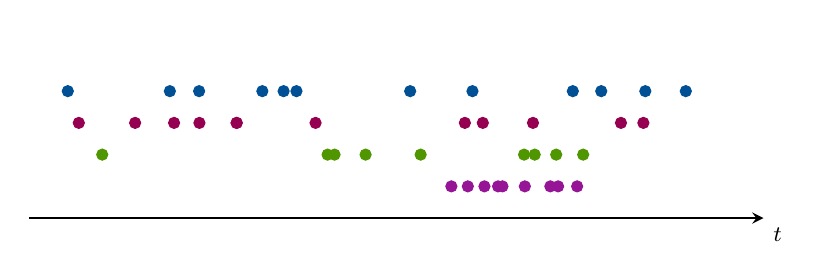
\begin{tikzpicture}
			\begin{axis}[
        width=0.9\columnwidth,
				xlabel=$t$,
				ymin = 0,
				ymax = .6,
				xmin = 0,
				xmax=22,
				xlabel style = {at={(axis cs:22,0)},anchor=north west},
				y axis line style={draw=none},
				x axis line style={->, thick},
				ticks=none,
				axis x line*=middle,
				height=4cm,
				]
			\addplot+[azulcito, mark options={fill=azulcito},mark=*,only marks] coordinates {
				(1.168317969682793,0.4)
				(4.224371806575089,0.4)
				(5.099828260436964,0.4)
				(6.9938720827411025,0.4)
				(7.629926439960695,0.4)
				(8.015139525296764,0.4)
				(11.41978663218779,0.4)
				(13.285132721106107,0.4)
				(16.28953436494327,0.4)
				(17.14081344555717,0.4)
				(18.46073553951872,0.4)
				(19.6728937320483,0.4)
			};
			\addplot+[rojito, mark options={fill=rojito},mark=*,only marks] coordinates {
				(1.49783995292964,.3)
  				(3.184138404294451,.3)
  				(4.35051050123616,.3)
  				(5.1091887517481505,.3)
  				(6.221541171374557,.3)
  				(6.226859317209702,.3)
  				(8.586778366165495,.3)
				(13.057655264423126,.3)
 				(13.594421727013588,.3)
 				(15.096680803679005,.3)
				(17.731518813017008,.3)
 				(18.40246895328477,.3)				
			};
      \addplot+[verdecito, mark options={fill=verdecito}, mark=*,only marks] coordinates {
				(2.1995364349536235,0.2)
				(8.947058606859512,0.2)
  				(9.155089124125874,0.2)
 				(10.084686662202682,0.2)
 				(11.733424911823171,0.2)
 				(14.830631279727431,0.2)
 				(15.149252788554351,0.2)
 				(15.791821681936792,0.2)
 				(16.599742636184,0.2)

			};
			\addplot+[violetita,mark options={fill=violetita},mark=*,only marks] coordinates {
				(12.653556737204989,0.1)
 				(13.146127585840045,0.1)
 				(13.643536674608884,0.1)
 				(14.051631664505377,0.1)
 				(14.183143031766923,0.1)
 				(14.85305783374829,0.1)
 				(15.61726438611725,0.1)
 				(15.848820745581179,0.1)
 				(16.419089799482926,0.1)
			};
			\end{axis}
		\end{tikzpicture}

		\item At each point in time we must decide which items must be stored locally.
	\end{itemize}
\end{block}

If inter-request times are \alert{heavy tailed}, this can model burstiness.
\end{frame}

\begin{frame}{Example: Pareto arrivals}

	Consider two items, with equal popularity...

	\vfill

	\begin{myitem}[1em]
		\item Poisson arrivals:
		
		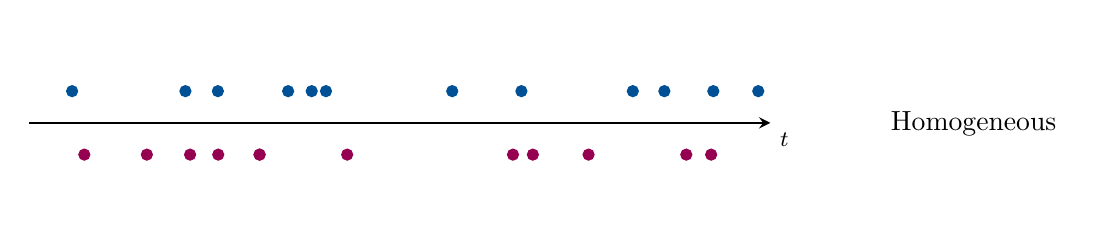
\begin{tikzpicture}
			\begin{axis}[
				xlabel=$t$,
				ymin = -.3,
				ymax = .3,
				xmin = 0,
				xmax=20,
				xlabel style = {at={(axis cs:20,0)},anchor=north west},
				y axis line style={draw=none},
				x axis line style={->, thick},
				ticks=none,
				axis x line*=middle,
				height=4cm,
				]
			\addplot+[azulcito, mark options={fill=azulcito},mark=*,only marks] coordinates {
				(1.168317969682793,0.1)
				(4.224371806575089,0.1)
				(5.099828260436964,0.1)
				(6.9938720827411025,0.1)
				(7.629926439960695,0.1)
				(8.015139525296764,0.1)
				(11.41978663218779,0.1)
				(13.285132721106107,0.1)
				(16.28953436494327,0.1)
				(17.14081344555717,0.1)
				(18.46073553951872,0.1)
				(19.6728937320483,0.1)
			};
			\addplot+[rojito, mark options={fill=rojito},mark=*,only marks] coordinates {
				(1.49783995292964,-.1)
  				(3.184138404294451,-.1)
  				(4.35051050123616,-.1)
  				(5.1091887517481505,-.1)
  				(6.221541171374557,-.1)
  				(6.226859317209702,-.1)
  				(8.586778366165495,-.1)
				(13.057655264423126,-.1)
 				(13.594421727013588,-.1)
 				(15.096680803679005,-.1)
				(17.731518813017008,-.1)
 				(18.40246895328477,-.1)				
			};
			\end{axis}
			\node at (12,1.2) {Homogeneous};
		\end{tikzpicture}

		\item Heavy tailed arrivals (Pareto $\alpha=2$):
		
		\begin{tikzpicture}
			\begin{axis}[
				xlabel=$t$,
				ymin = -.3,
				ymax = .3,
				xmin = 0,
				xmax=20,
				xlabel style = {at={(axis cs:20,0)},anchor=north west},
				y axis line style={draw=none},
				x axis line style={->, thick},
				ticks=none,
				axis x line*=middle,
				height=4cm,
				]
			\addplot+[azulcito, mark options={fill=azulcito}, mark=*,only marks] coordinates {
				(2.1995364349536235,.1)
				(8.947058606859512,.1)
  				(9.155089124125874,.1)
 				(10.084686662202682,.1)
 				(11.733424911823171,.1)
 				(14.830631279727431,.1)
 				(15.149252788554351,.1)
 				(15.791821681936792,.1)
 				(16.599742636184,.1)

			};
			\addplot+[rojito,mark options={fill=rojito},mark=*,only marks] coordinates {
				(12.653556737204989,-.1)
 				(13.146127585840045,-.1)
 				(13.643536674608884,-.1)
 				(14.051631664505377,-.1)
 				(14.183143031766923,-.1)
 				(14.85305783374829,-.1)
 				(15.61726438611725,-.1)
 				(15.848820745581179,-.1)
 				(16.419089799482926,-.1)
			};
			\end{axis}
			\node at (12,1.2) {Bursty!};
		\end{tikzpicture}

	\end{myitem}

\end{frame}

\begin{frame}{Some open questions...}

  \begin{myitem}[2em]

    \item What is the optimal causal policy in this framework?
    
    \item Can we compute the optimal hit rate/hit probability?
    
    \item What is its large scale behavior?
    
    \item How typical policies compare to the optimal one?
  \end{myitem}

\end{frame}

\section{Point processes and stochastic intensity}

\begin{frame}{A bit of point process theory...}
	
	Let $\Phi = \{\tau_k:k\in\mathbb{Z}\}$ be a \alert{stationary point process} representing request times:

	\begin{center}

	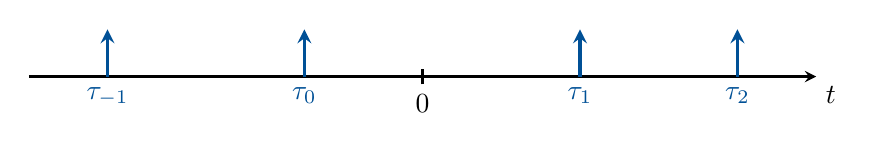
\begin{tikzpicture}
	   
		\draw[->,thick] (-5,0) -- (5,0);
		\node[below right] at (5,0) {$t$};
		
		\draw[<-,very thick, azulcito] (-4,.6) -- (-4,0) node[below] {$\tau_{-1}$};
		\draw[<-,very thick, azulcito] (-1.5,.6) -- (-1.5,0) node[below] {$\tau_{0}$};
		\draw[<-,very thick, azulcito] (2,.6) -- (2,0) node[below] {$\tau_{1}$};
		\draw[<-,very thick, azulcito] (4,.6) -- (4,0) node[below] {$\tau_{2}$};
		\draw[-,thick] (0,-.1) node[below] {$0$} -- (0,0.1);
		 
	\end{tikzpicture}

	\end{center}
	i.e. $\Phi(B) = \sum_k \ind{\{\tau_k\in B\}}$ is a \emph{random counting measure}.

	\pause \vfill

	\begin{columns}
		\begin{column}{0.4\textwidth}
			\alert{Counting process:}
			\begin{equation*}
				\Phi(t) = \begin{cases}
					\Phi((0,t]) & t > 0 \\
					-\Phi((t,0]) & t\leqslant 0
				\end{cases}
			\end{equation*}

			\vfill
			{\small \alert{Note:} $\Phi(\tau_k) = k$}
		\end{column}
		\begin{column}{0.6\textwidth}
			\begin{tikzpicture}
				\begin{axis}[
					width=\columnwidth,
					height= 0.5\columnwidth,
					xlabel=$t$,
					ymin = -2.1,
					ymax = 2.1,
					xmin = -5,
					xmax=5,
					xlabel style = {at={(axis cs:7,0)},anchor=north west},
					y axis line style={draw=none},
					x axis line style={->, thick},
					xtick={0},
					ymajorticks=false,
					axis x line*=middle,
					]
		
					\addplot+[azulcito, mark options={fill=azulcito, scale=1.5}, mark=*,only marks] coordinates {
						(-4,0)
						(-1.5,0)
						(2,0)
						(4,0)
					};
					\addplot+[rojito, const plot, no marks, very thick] coordinates {
						(-5,-2)
						(-4,-1)
						(-1.5,-0)
						(2,1)
						(4,2)
						(5,2)
					};
					\node[above left, rojito] at (axis cs:4,1) {$\Phi(t)$};
				\end{axis}
			\end{tikzpicture}
		\end{column}
	\end{columns}
	\pause \vfill

	Let $\mathcal{F}_t = \sigma(N(s), s\leqslant t)$ be its \alert{internal history}.
\end{frame}

	\begin{frame}{Two important distributions:}

		\begin{center}

			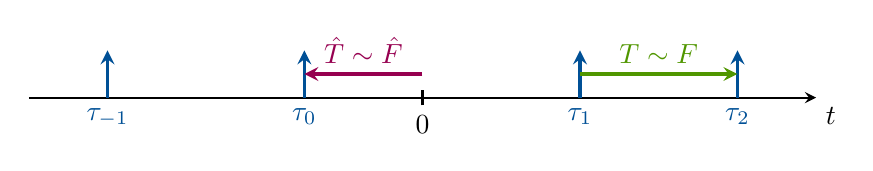
\begin{tikzpicture}
			   
				\draw[->,thick] (-5,0) -- (5,0);
				\node[below right] at (5,0) {$t$};
				
				\draw[<-,very thick, azulcito] (-4,.6) -- (-4,0) node[below] {$\tau_{-1}$};
				\draw[<-,very thick, azulcito] (-1.5,.6) -- (-1.5,0) node[below] {$\tau_{0}$};
				\draw[<-,very thick, azulcito] (2,.6) -- (2,0) node[below] {$\tau_{1}$};
				\draw[<-,very thick, azulcito] (4,.6) -- (4,0) node[below] {$\tau_{2}$};
				\draw[-,thick] (0,-.1) node[below] {$0$} -- (0,0.1);
				 
				\draw[->, very thick, verdecito] (2,.3) -- node[midway, above, anchor=south] {$T\sim F$} (4,.3);
		
				\draw<2->[->, very thick, rojito] (0,.3) -- node[midway, above, anchor=south] {$\hat{T}\sim \hat{F}$} (-1.5,.3);
		
			\end{tikzpicture}
		
		\end{center}

		\vfill

		\begin{tabular}{m{4cm} m{6cm}}
			\alert{Inter-arrival distribution:} & 
					\begin{gather*}
						F(t) := P^0_N (\tau_1 - \tau_0 \leqslant t), \quad
						E^0_\Phi[\tau_1] = 1/\lambda.
					\end{gather*} \\[-2em]
					\uncover<2->{
			\alert{Age distribution:} &
					\begin{equation*}
						\hat{F}(t) := P (- \tau_0 \leqslant t) = \lambda \int_0^t 1-F(s)ds,
					\end{equation*}}
		\end{tabular}

			\vfill

		Note: here $P^0_\Phi$ is the \alert{Palm probability} of the point process (conditioning on $\tau_0=0$).

\end{frame}

\begin{frame}{Stochastic intensity}
	Consider a simple stationary point process $\Phi$ with intensity $\lambda$, defined in some probability space $(\Omega, \mathcal{F},P)$. Let some filtration $\{\mathcal{F}_t\}_{t\in\mathbb{R}}$ be a \alert{history} of the process.

	\bigskip

	\begin{block}{Definition:}

		The random process $\lambda(t)\geqslant 0$ is a \alert{stochastic intensity} for the history $\mathcal{F}_t$ iff it is a.s. locally integrable, $\mathcal{F}_t-$adapted and:
		\begin{equation*}
			\E{\Phi((a,b])\mid \mathcal{F}_a} = \E{\left.\int_a^b \lambda(t)dt \right| \mathcal{F}_a}
		\end{equation*}
		for all $a,b\in \mathbb{R}$.
	\end{block}

\end{frame}

\begin{frame}{Stochastic intensity}{Properties}

	
	\alert{Local interpretation:}
		\begin{equation*}
			E[\Phi((t,t+h])\mid \mathcal{F}_t] = \lambda(t)h + o(h) \quad P-a.s.,
		\end{equation*}
	
	So $\lambda(t)$ acts as a \alert{local} notion of intensity based on previous history.

	\pause \vfill
	\alert{Martingale interpretation:}
		\begin{equation*}
			M_a(t) = \Phi(t) - \Phi(a) - \int_a^t \lambda(s)ds
		\end{equation*} 
		is a local $(P,\mathcal{F}_t)$ martingale for any $a\in\mathbb{R}$.
	
	% 	\vfill

	% Namely, $A(t) = N(a) + \int_a^t \lambda(s)ds$ is the \alert{compensator} of the counting process.

\end{frame}

\begin{frame}{Stochastic intensity of a Poisson process}

	\begin{myitem}[2em]
		\item If $\Phi(t)$ is a Poisson process, then we know that
		\begin{equation*}
			M(t) = \Phi(t) - \lambda t = \Phi(t) - \int_0^t \lambda dt
		\end{equation*}
		is a martingale, so the stochastic intensity of a Poisson process is just $\lambda(t)\equiv \lambda$.

		% \item In fact, this \alert{characterizes} the Poisson process. The stochastic intensity $\lambda(t)$ is \alert{deterministic} if and only if $N$ is a Poisson process of (possible time-varying) intensity $\lambda(t)$.
	\end{myitem}

	\pause \vfill
	\centering
	The poisson process is the \alert{``white noise''} of point processes.

	\vfill
\end{frame}

\begin{frame}{Stochastic intensity}{A local notion of intensity...}
	
	However, if traffic is \alert{bursty}, the stochastic intensity \alert{rises} after arrivals:

	\vfill

	\begin{center}
	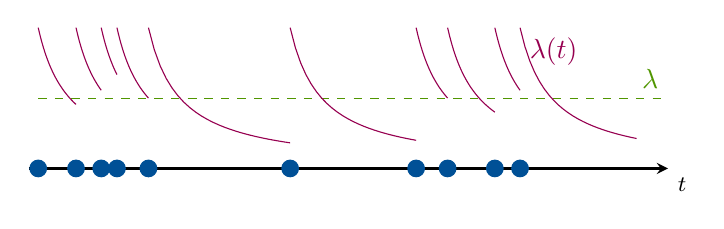
\begin{tikzpicture}
		\begin{axis}[xlabel=$t$,
			ymin = -.3,
			ymax = 2,
			xmin = -.3,
			xmax=20,
			xlabel style = {at={(axis cs:20,0)},anchor=north west},
			y axis line style={draw=none},
			x axis line style={->, thick},
			ticks=none,
			axis x line*=middle,
			width=0.8\textwidth,
			height= 0.3\textwidth,
			]
			\addplot[verdecito,domain=0:20, dashed] {1};
			\addplot[rojito,domain=0:1.2] {2/(1+x)};
			\addplot[rojito,domain=1.2:2] {2/(1+x-1.2)};
			\addplot[rojito,domain=2:2.5] {2/(1+x-2)};
			\addplot[rojito,domain=2.5:3.5] {2/(1+x-2.5)};
			\addplot[rojito,domain=3.5:8] {2/(1+x-3.5)};
			\addplot[rojito,domain=8:12] {2/(1+x-8)};
			\addplot[rojito,domain=12:13] {2/(1+x-12)};
			\addplot[rojito,domain=13:14.5] {2/(1+x-13)};
			\addplot[rojito,domain=14.5:15.3] {2/(1+x-14.5)};
			\addplot[rojito,domain=15.3:19] {2/(1+x-15.3)};
			\node[below right, rojito] at (axis cs:15.3,2) {$\lambda(t)$};
			\node[above left, verdecito] at (axis cs:20,1) {$\lambda$};

			\addplot+[azulcito, mark options={fill=azulcito, scale=1.5}, mark=*,only marks] coordinates {
				(0,0)
				(1.2,0)
 				(2,0)
 				(2.5,0)
 				(3.5,0)
 				(8,0)
 				(12,0)
 				(13,0)
 				(14.5,0)
 				(15.3,0)
			};
		\end{axis}
	\end{tikzpicture}
	\end{center}

	\vfill
	Note: for stationary processes, $E[\lambda(t)] = E[\lambda(0)] = \lambda$, the average intensity.
\end{frame}

\begin{frame}{Renewal processes}

	\begin{itemize}
	\item Let now $\Phi$ be a \alert{stationary renewal process}, i.e. inter request times $\tau_{k+1}-\tau_k$ are $iid\sim F$.
	
	\item Assume that $F$ has a density, and define the \alert{hazard rate} of $F$ as:
	 \begin{equation*}
		\eta(t) = \frac{f(t)}{1-F(t)}
	 \end{equation*}

	\end{itemize}
	\pause
	 \begin{theorem}[Daley-Vere Jones, Chapter 7]
		For a renewal process and its natural history, the stochastic intensity is:
		\begin{equation*}
			\lambda(t) = \eta(t-\tau^-(t)),
		\end{equation*}
		where $\tau^-(t)$ is the last point before $t$:
		\begin{equation*}
			\tau^-(t) = \sup\{\tau_k:\tau_k<t\}
		\end{equation*}
	\end{theorem}

\end{frame}

\begin{frame}{Some examples...}

	\begin{tabular}{m{7cm} m{6cm}}

		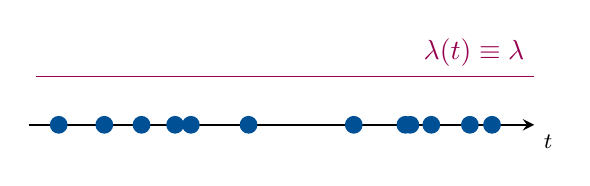
\begin{tikzpicture}
			\begin{axis}[xlabel=$t$,
				ymin = -.3,
				ymax = 2,
				xmin = -.3,
				xmax=20,
				xlabel style = {at={(axis cs:20,0)},anchor=north west},
				y axis line style={draw=none},
				x axis line style={->, thick},
				ticks=none,
				axis x line*=middle,
				width=8cm,
				height= 3cm,
				]
				\addplot[rojito, domain=0:20] {1};
				\node[above left, rojito] at (axis cs:20,1) {$\lambda(t)\equiv \lambda$};
	
				\addplot+[azulcito, mark options={fill=azulcito, scale=1.5}, mark=*,only marks] coordinates {
					(0.9028581008067987,0)
					(2.7341797790213573,0)
					(4.228330726726128,0)
					(5.577074925845067,0)
					(6.211423990911654,0)
					(8.528255357570485,0)
					(12.753859672976413,0)
					(14.826517141978712,0)
					(15.028110470502309,0)
					(15.868264106338712,0)
					(17.418133532477547,0)
					(18.306210880027027,0)
				};
			\end{axis}
		\end{tikzpicture} & \alert{Constant hazard rate} $\to$ Poisson process.\\
		\\
		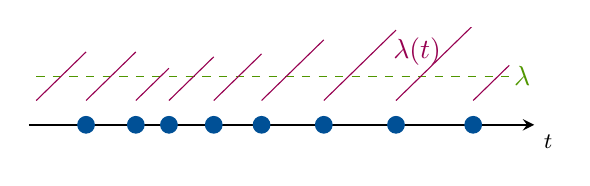
\begin{tikzpicture}
			\begin{axis}[xlabel=$t$,
				ymin = -.3,
				ymax = 2,
				xmin = -.3,
				xmax=20,
				xlabel style = {at={(axis cs:20,0)},anchor=north west},
				y axis line style={draw=none},
				x axis line style={->, thick},
				ticks=none,
				axis x line*=middle,
				width=8cm,
				height=3cm,
				]
				\addplot[verdecito,domain=0:19, dashed] {1};
				\addplot[rojito,domain=0:2] {0.5+0.5*x};
				\addplot[rojito,domain=2:4] {0.5+0.5*(x-2};
				\addplot[rojito,domain=4:5.33] {0.5+0.5*(x-4};
				\addplot[rojito,domain=5.33:7.13] {0.5+0.5*(x-5.33};
				\addplot[rojito,domain=7.13:9.05] {0.5+0.5*(x-7.13};
				\addplot[rojito,domain=9.05:11.55] {0.5+0.5*(x-9.05};
				\addplot[rojito,domain=11.55:14.45] {0.5+0.5*(x-11.55};
				\addplot[rojito,domain=14.45:17.55] {0.5+0.5*(x-14.45};
				\addplot[rojito,domain=17.55:19] {0.5+0.5*(x-17.55};
				\node[below, rojito] at (axis cs:15.3,2) {$\lambda(t)$};
				\node[right, verdecito] at (axis cs:18.8,1) {$\lambda$};

				\addplot+[azulcito, mark options={fill=azulcito, scale=1.5}, mark=*,only marks] coordinates {
					(2,0)
					(4,0)
					(5.33,0)
					(7.13,0)
					(9.05,0)
					(11.55,0)
					(14.45,0)
					(17.55,0)
				};
			\end{axis}
		\end{tikzpicture} & \alert{Increasing} hazard rate $\to$ more periodic!\\
		\\
		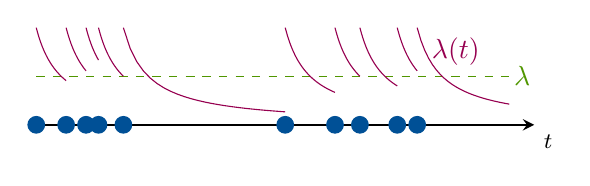
\begin{tikzpicture}
			\begin{axis}[xlabel=$t$,
				ymin = -.3,
				ymax = 2,
				xmin = -.3,
				xmax=20,
				xlabel style = {at={(axis cs:20,0)},anchor=north west},
				y axis line style={draw=none},
				x axis line style={->, thick},
				ticks=none,
				axis x line*=middle,
				width=8cm,
				height=3cm,
				]
				\addplot[verdecito,domain=0:19, dashed] {1};
				\addplot[rojito,domain=0:1.2] {2/(1+x)};
				\addplot[rojito,domain=1.2:2] {2/(1+x-1.2)};
				\addplot[rojito,domain=2:2.5] {2/(1+x-2)};
				\addplot[rojito,domain=2.5:3.5] {2/(1+x-2.5)};
				\addplot[rojito,domain=3.5:10] {2/(1+x-3.5)};
				\addplot[rojito,domain=10:12] {2/(1+x-10)};
				\addplot[rojito,domain=12:13] {2/(1+x-12)};
				\addplot[rojito,domain=13:14.5] {2/(1+x-13)};
				\addplot[rojito,domain=14.5:15.3] {2/(1+x-14.5)};
				\addplot[rojito,domain=15.3:19] {2/(1+x-15.3)};
				\node[below right, rojito] at (axis cs:15.5,2) {$\lambda(t)$};
				\node[right, verdecito] at (axis cs:18.8,1) {$\lambda$};
	
				\addplot+[azulcito, mark options={fill=azulcito, scale=1.5}, mark=*,only marks] coordinates {
					(0,0)
					(1.2,0)
					 (2,0)
					 (2.5,0)
					 (3.5,0)
					 (10,0)
					 (12,0)
					 (13,0)
					 (14.5,0)
					 (15.3,0)
				};
			\end{axis}
		\end{tikzpicture} & \alert{Decreasing} hazard rate $\to$ more bursty!


	\end{tabular}
\end{frame}


\section{The optimal caching policy}

% \begin{frame}{The predictable $\sigma-$algebra}

% 	Let $(\Omega,\mathcal{F},\{\mathcal{F}_t: t\in\mathbb{R}\},P)$ be a filtered probability space.

% 	\bigskip

% 	\begin{definition}
% 		The predictable $\sigma-$algebra $\mathcal{P}(\mathcal{F}.)$ is the $\sigma-$álgebra in $\mathbb{R}\times \Omega$ generated by the sets:
% 		\begin{equation*}
% 			(a,b] \times A, \; a<b, \; A\in\mathcal{F}_a, 
% 		\end{equation*}
% 	\end{definition}

% \end{frame}

% \begin{frame}{Predictable processes}

% 	\begin{definition}[Predictable process]
% 		A stochastic process $X(t,\omega)$ taking values on a measurable space $(E,\mathcal{E})$ is \alert{$\mathcal{F}_t-$predictable} if the mapping $(t,\omega) \mapsto X(t,\omega)$ is $\mathcal{P}(\mathcal{F}.)-$measurable.
% 	\end{definition}

% 	\vfill
% 	\begin{myitem}
% 		\item \alert{Key idea:} a process is $\mathcal{F}_t-$predictable if its value at $t$ is completely determined by the information prior to $t$.
% 		\pause
% 		\item In particular $\mathcal{F}_t-$adapted $+$ left continuous $\Longrightarrow$ $\mathcal{F}_t$-predictable.
		
% 		\item Since the stochastic intensity of a point process can be chosen left-continuous, it is $\mathcal{F}_t$-predictable.
% 	\end{myitem}

% \end{frame}

\begin{frame}{Causal caching policies}
	
	\begin{myitem}[1em]
		\item Consider again a cache system fed by $N$ \alert{independent} request processes $\Phi_i(t)$ with stochastic intensities $\lambda_i(t)$.
		\item Let $\mathcal{F}_t = \sigma(\{\mathcal{F}_t^{(i)}: i=1,\ldots,M\})$ their aggregate history.
	\end{myitem}

	\vfill

	\begin{block}{Definition}
		A \alert{causal} caching policy is an $\mathcal{F}_t$ \alert{predictable} stochastic process
		\begin{equation*}
			\pi(t):\Omega\times\mathbb{R} \to \mathcal{C}
		\end{equation*}
		i.e. $\pi(t) = \{i_1,\ldots,i_k\}$ (with $k\leqslant C$) is the subset kept at time $t$, and only depends on the past history of item requests.
	\end{block}

\end{frame}

\begin{frame}{The hit process}{Stochastic intensity}
	
	Focus now on a particular content $i$, its \alert{hit process} is the point process given by:

	\vfill

	\begin{columns}
		\begin{column}{0.5\textwidth}
			\begin{equation*}
				H_i(B) = \sum_{k\in\mathbb{Z}} \ind{\{\tau_k^i\in B\}}\ind{\{i\in \pi(\tau_k^i)\}}
			\end{equation*}
		\end{column}
		\begin{column}{0.5\textwidth}
			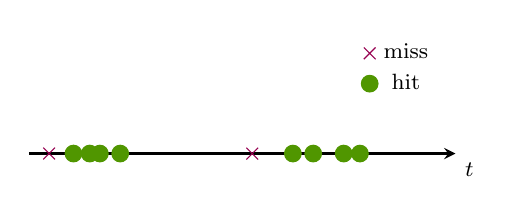
\begin{tikzpicture}
				\begin{axis}[xlabel=$t$,
					ymin = -.3,
					ymax = 1.5,
					xmin = -1,
					xmax=20,
					xlabel style = {at={(axis cs:20,0)},anchor=north west},
					y axis line style={draw=none},
					x axis line style={->, thick},
					ticks=none,
					axis x line*=middle,
					width=7cm,
					height=3.5cm,
					legend pos=north east
					]
					\addplot+[rojito, mark options={fill=rojito, scale=1.5}, mark=x,only marks] coordinates {
						(0,0)
						 (10,0)
					};
					\addlegendentry{miss}
					\addplot+[verdecito, mark options={fill=verdecito, scale=1.5}, mark=*,only marks] coordinates {
						(1.2,0)
						 (2,0)
						 (2.5,0)
						 (3.5,0)
						 (12,0)
						 (13,0)
						 (14.5,0)
						 (15.3,0)
					};
					\addlegendentry{hit}
				\end{axis}
			\end{tikzpicture}

		\end{column}
	\end{columns}

	\vfill

	Now $\ind{\{i\in \pi(t)\}}$ is $\mathcal{F}_t$-predictable, so the stochastic intensity of $H_i$ is:
	\begin{equation*}
		h_i(t) = \lambda_i(t) \ind{\{i\in \pi(t)\}}
	\end{equation*}
	i.e., $h_i(t)=\lambda_i(t)$ while $i$ is cached and otherwise $0$.
\end{frame}

\begin{frame}{The hit process}{The hit rate}
	If we now consider the aggregate of requests, the \alert{total hit process} is given by:
	\begin{equation*}
		H = \sum_{i=1}^N H_i
	\end{equation*}

	And its stochastic intensity is just:
	\begin{equation*}
		h(t) = \sum_{i=1}^N h_i(t) = \sum_{i=1}^N \lambda_i(t) \ind{\{i\in \pi(t)\}}
	\end{equation*}

	The steady state \alert{hit rate} of the policy is:
	\begin{equation*}
		\text{hit rate} = \lambda_{\text{hit}} := E[h(0)]
	\end{equation*}
	
\end{frame}

\begin{frame}{Maximizing the hit rate}
	
	In order to maximize $\lambda_{\text{hit}}$, consider the causal policy:
	\begin{equation*}
		\pi^*(t) = \{i_1,\ldots,i_C\} \quad \text{such that}\; \sum_{i\in\{i_1,\ldots,i_C\}} \lambda_{i}(t) \text{ is maximized.}
	\end{equation*}

	Then, for any causal policy $\pi$ and for each realization:
	\begin{equation*}
		h(t) = \sum_{i\in\pi(t)} \lambda_i(t) \leqslant \sum_{i\in \pi^*(t)} \lambda_i(t) = h^*(t).
	\end{equation*} 

	\begin{theorem}
		The \alert{optimal causal policy} is to keep in the cache the $C$ objects with the \alert{highest stochastic intensity} at any time.
	\end{theorem}

\end{frame}

\begin{frame}{Back to the Poisson case}

	\begin{myitem}
		\item Assume the $\Phi_i$ are Poisson processes of intensities $\lambda_i$.
		\item We take $\lambda_1>\lambda_2>\ldots$ as the popularities.
		\item The total request process is also Poisson of intensity $\sum_i\lambda_i$.
		\item In that case, the optimal policy is:
		\begin{equation*}
			\pi^*(t) \equiv \{1,\ldots,C\}
		\end{equation*}
		since $\lambda_i(t)\equiv \lambda_i$ and these are is decreasing.
	\end{myitem}

	\pause \vfill
	\alert{Conclusion:} under Poisson arrivals, statically keeping the most popular objects is optimal (compare to the IRM before).
\end{frame}

\begin{frame}{The Renewal case}
	\begin{myitem}[2em]
		\item If now the $\Phi_i$ are renewal processes of (decreasing) intensities $\lambda_i$.
		\item The total request process is no longer renewal, but its intensity is again $\sum_i\lambda_i$.
		\item Since $\lambda_i(t) = \eta_i(t-T^*_i(t))$, the optimal policy is:
		\vspace{1em}
		\begin{itemize}
			\item Keep track of the \alert{current hazard rate} of each content $i$.
			\vspace{.5em}
			\item Choose to keep in $\pi^*(t)$ the $C$ highest. 
		\end{itemize}
	\end{myitem}

	\pause \vfill
	\alert{Conclusion:} under renewal arrivals, the optimal policy only depends on the current hazard rates since the last request.
\end{frame}

\begin{frame}{An interesting observation}

	\alert{Decreasing hazard rates}

	\begin{myitem}[1em]
		\item If hazard rates are \alert{decreasing}, caching makes sense! After an arrival it becomes more likely to get another request.
		\item After some time, we will evict the content to make room for more recent ones (as in LRU).
	\end{myitem}

	\pause\vfill
	\alert{Increasing hazard rates}

	\begin{myitem}[1em]
		\item If instead hazard rates are \alert{increasing}, then when a request arrives, the item becomes less likely to be requested again! 
		\item It may be better to remove it and make room for other ones (i.e. LRU makes no sense!).
		\item If we haven't seen it for a while, then we may have to fetch it \alert{anticipating} the upcoming request.
	\end{myitem}
\end{frame}

\section{Large scale asymptotics}

\begin{frame}{Understanding the optimal policy}{The threshold process}
	
	We can rewrite this optimal policy as a \alert{threshold} policy:

	\begin{equation*}
		i\in\pi^*(t) \Leftrightarrow \lambda_i(t) \geqslant \theta(t) := \text{ the $C$ largest stochastic intensity}
	\end{equation*}

	\vfill
	\alert{Example:} Pareto requests, Zipf popularities, $N=20, C=4$.
	\begin{center}
		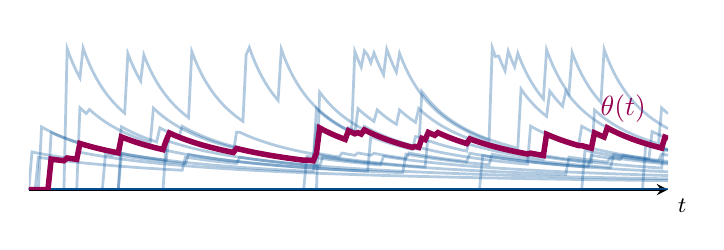
\begin{tikzpicture}
\begin{axis}[
    width = 0.8\textwidth,
    height = 0.3\textwidth,
    xlabel=$t$,
	ymin = 0,
	ymax = .3,
	xmin = 0,
	xmax=100,
	xlabel style = {at={(axis cs:100,0)},anchor=north west},
				y axis line style={draw=none},
				x axis line style={->, thick},
				ticks=none,
				axis x line*=middle,
]

    \node[rojito] at (axis cs:93,0.15) {$\theta(t)$};
    \addplot[color=azulcito, draw opacity=0.3, line width={1}, solid]
        table[row sep={\\}]
        {
            \\
            0.0  0.0  \\
            0.5  0.0  \\
            1.0  0.0  \\
            1.5  0.0  \\
            2.0  0.0  \\
            2.5  0.0  \\
            3.0  0.0  \\
            3.5  0.0  \\
            4.0  0.0  \\
            4.5  0.0  \\
            5.0  0.0  \\
            5.5  0.0  \\
            6.0  0.2611738739465073  \\
            6.5  0.24516612714948413  \\
            7.0  0.2310073338063749  \\
            7.5  0.21839464277037962  \\
            8.0  0.20708791970867058  \\
            8.5  0.26224694410648997  \\
            9.0  0.2461114501768651  \\
            9.5  0.23184643461641943  \\
            10.0  0.21914446868385415  \\
            10.5  0.20776199564668177  \\
            11.0  0.19750356209465342  \\
            11.5  0.18821050100178544  \\
            12.0  0.17975266616304697  \\
            12.5  0.17202229942285782  \\
            13.0  0.1649294151152114  \\
            13.5  0.15839828114892462  \\
            14.0  0.15236470433049598  \\
            14.5  0.14677391335264464  \\
            15.0  0.14157889136905338  \\
            15.5  0.2520912551632043  \\
            16.0  0.23714566789421224  \\
            16.5  0.22387303763580027  \\
            17.0  0.2120073549948435  \\
            17.5  0.2013361678900516  \\
            18.0  0.24948282992194729  \\
            18.5  0.23483594583817125  \\
            19.0  0.22181350006623865  \\
            19.5  0.21015944931035774  \\
            20.0  0.19966887415134146  \\
            20.5  0.19017582588978763  \\
            21.0  0.18154448289711436  \\
            21.5  0.1736626106833466  \\
            22.0  0.16643665469156177  \\
            22.5  0.15978800926124526  \\
            23.0  0.15365014650313658  \\
            23.5  0.1479663824190789  \\
            24.0  0.14268812114411153  \\
            24.5  0.13777346203382987  \\
            25.0  0.13318608502661755  \\
            25.5  0.25588903660117995  \\
            26.0  0.24050348531223642  \\
            26.5  0.22686314127109147  \\
            27.0  0.21468699949709727  \\
            27.5  0.2037513101425696  \\
            28.0  0.1938757030188443  \\
            28.5  0.18491316075894978  \\
            29.0  0.17674265023498373  \\
            29.5  0.16926362482499627  \\
            30.0  0.16239186586058207  \\
            30.5  0.1560562975269098  \\
            31.0  0.15019651934914569  \\
            31.5  0.14476087447801167  \\
            32.0  0.1397049227803694  \\
            32.5  0.13499022310656741  \\
            33.0  0.13058335408121077  \\
            33.5  0.12645512063296172  \\
            34.0  0.24959046979880165  \\
            34.5  0.2632891709905496  \\
            35.0  0.24702914621142247  \\
            35.5  0.23266065544361586  \\
            36.0  0.2198717774782077  \\
            36.5  0.20841560035229592  \\
            37.0  0.198094123911953  \\
            37.5  0.18874671988284142  \\
            38.0  0.18024171190577087  \\
            38.5  0.17247013386084672  \\
            39.0  0.1653410361993485  \\
            39.5  0.25992505788788384  \\
            40.0  0.2440653808278566  \\
            40.5  0.2300298029624121  \\
            41.0  0.217520739736931  \\
            41.5  0.20630199888524928  \\
            42.0  0.19618372521984706  \\
            42.5  0.1870115686696426  \\
            43.0  0.17865875515511184  \\
            43.5  0.1710201915240911  \\
            44.0  0.16400802074429693  \\
            44.5  0.15754822750315572  \\
            45.0  0.15157801558229658  \\
            45.5  0.14604375975917816  \\
            46.0  0.14089939057243436  \\
            46.5  0.13610510884975302  \\
            47.0  0.13162635403876738  \\
            47.5  0.12743296974093446  \\
            48.0  0.12349852382841536  \\
            48.5  0.11979975073569768  \\
            49.0  0.11631609105690562  \\
            49.5  0.1130293092016073  \\
            50.0  0.1099231740933524  \\
            50.5  0.10698319110804443  \\
            51.0  0.25611727584669625  \\
            51.5  0.2407050926910798  \\
            52.0  0.22704251998653593  \\
            52.5  0.2569544147897623  \\
            53.0  0.24955147933559932  \\
            53.5  0.23489677021125602  \\
            54.0  0.25323697640522397  \\
            54.5  0.238159291673662  \\
            55.0  0.22477615897217698  \\
            55.5  0.21281710605644164  \\
            56.0  0.26013520810937735  \\
            56.5  0.244250659100394  \\
            57.0  0.23019437702311868  \\
            57.5  0.21766789561581476  \\
            58.0  0.25239974035179097  \\
            58.5  0.23741863960410323  \\
            59.0  0.22411629324053284  \\
            59.5  0.21222549540046107  \\
            60.0  0.2015328909928499  \\
            60.5  0.19186606052747224  \\
            61.0  0.18308415179022133  \\
            61.5  0.1750709717009804  \\
            62.0  0.16772981622360697  \\
            62.5  0.1609795486940538  \\
            63.0  0.15475158847591844  \\
            63.5  0.1489875725953433  \\
            64.0  0.14363752119136491  \\
            64.5  0.13865838452979995  \\
            65.0  0.1340128820954167  \\
            65.5  0.12966856748398836  \\
            66.0  0.12559706946457386  \\
            66.5  0.12177347166951911  \\
            67.0  0.11817580224290675  \\
            67.5  0.11478461135976178  \\
            68.0  0.11158261945752762  \\
            68.5  0.10855442274658661  \\
            69.0  0.10568624540601076  \\
            69.5  0.1029657300523308  \\
            70.0  0.10038175975797639  \\
            70.5  0.09792430621279652  \\
            71.0  0.09558429965564282  \\
            71.5  0.09335351701946855  \\
            72.0  0.09122448538228663  \\
            72.5  0.2627283845681604  \\
            73.0  0.24653542132244147  \\
            73.5  0.24742802713694648  \\
            74.0  0.23301445068038476  \\
            74.5  0.22018772049590488  \\
            75.0  0.2565430858533927  \\
            75.5  0.24108115969131177  \\
            76.0  0.22737707731946255  \\
            76.5  0.25254075146019606  \\
            77.0  0.23754340402121352  \\
            77.5  0.2242274651825838  \\
            78.0  0.21232518090537242  \\
            78.5  0.2016227824649915  \\
            79.0  0.19194753351628033  \\
            79.5  0.1831583358155929  \\
            80.0  0.17513880289676617  \\
            80.5  0.16779207702053173  \\
            81.0  0.2590184623615969  \\
            81.5  0.24326587419202964  \\
            82.0  0.22931947363618876  \\
            82.5  0.21688545882208293  \\
            83.0  0.2057304718754835  \\
            83.5  0.19566681531424052  \\
            84.0  0.18654180508333407  \\
            84.5  0.17822997000229016  \\
            85.0  0.2536675035988033  \\
            85.5  0.2385400395157249  \\
            86.0  0.22511528714305062  \\
            86.5  0.21312108365712282  \\
            87.0  0.2023403357514016  \\
            87.5  0.1925977618042895  \\
            88.0  0.18375028824268114  \\
            88.5  0.17567997665545432  \\
            89.0  0.16828873633766028  \\
            89.5  0.16149431767581635  \\
            90.0  0.2597404598237086  \\
            90.5  0.24390261545132547  \\
            91.0  0.2298852142019637  \\
            91.5  0.21739144450550793  \\
            92.0  0.20618569309114462  \\
            92.5  0.19607854539547714  \\
            93.0  0.18691599146602428  \\
            93.5  0.17857152314209843  \\
            94.0  0.17094025760058848  \\
            94.5  0.16393450593217088  \\
            95.0  0.15748038851103038  \\
            95.5  0.15151521959908099  \\
            96.0  0.14598546466483925  \\
            96.5  0.14084512925482787  \\
            97.0  0.13605447666686718  \\
            97.5  0.13157899871426235  \\
            98.0  0.12738858315932905  \\
            98.5  0.12345683532595216  \\
            99.0  0.11976052157819485  \\
            99.5  0.11627910986662601  \\
            100.0  0.11299438814817749  \\
        }
        ;
    \addplot[color=azulcito, draw opacity=0.3, line width={1}, solid]
        table[row sep={\\}]
        {
            \\
            0.0  0.0  \\
            0.5  0.0  \\
            1.0  0.0  \\
            1.5  0.0  \\
            2.0  0.0  \\
            2.5  0.0  \\
            3.0  0.0  \\
            3.5  0.0  \\
            4.0  0.0  \\
            4.5  0.0  \\
            5.0  0.0  \\
            5.5  0.0  \\
            6.0  0.0  \\
            6.5  0.0  \\
            7.0  0.0  \\
            7.5  0.0  \\
            8.0  0.0  \\
            8.5  0.0  \\
            9.0  0.0  \\
            9.5  0.0  \\
            10.0  0.0  \\
            10.5  0.0  \\
            11.0  0.0  \\
            11.5  0.0  \\
            12.0  0.0  \\
            12.5  0.0  \\
            13.0  0.0  \\
            13.5  0.0  \\
            14.0  0.0  \\
            14.5  0.0  \\
            15.0  0.0  \\
            15.5  0.0  \\
            16.0  0.0  \\
            16.5  0.0  \\
            17.0  0.0  \\
            17.5  0.0  \\
            18.0  0.0  \\
            18.5  0.0  \\
            19.0  0.0  \\
            19.5  0.0  \\
            20.0  0.0  \\
            20.5  0.0  \\
            21.0  0.0  \\
            21.5  0.0  \\
            22.0  0.0  \\
            22.5  0.0  \\
            23.0  0.0  \\
            23.5  0.0  \\
            24.0  0.0  \\
            24.5  0.0  \\
            25.0  0.0  \\
            25.5  0.0  \\
            26.0  0.0  \\
            26.5  0.0  \\
            27.0  0.0  \\
            27.5  0.0  \\
            28.0  0.0  \\
            28.5  0.0  \\
            29.0  0.0  \\
            29.5  0.0  \\
            30.0  0.0  \\
            30.5  0.0  \\
            31.0  0.0  \\
            31.5  0.0  \\
            32.0  0.0  \\
            32.5  0.0  \\
            33.0  0.0  \\
            33.5  0.0  \\
            34.0  0.0  \\
            34.5  0.0  \\
            35.0  0.0  \\
            35.5  0.0  \\
            36.0  0.0  \\
            36.5  0.0  \\
            37.0  0.0  \\
            37.5  0.0  \\
            38.0  0.0  \\
            38.5  0.0  \\
            39.0  0.0  \\
            39.5  0.0  \\
            40.0  0.0  \\
            40.5  0.0  \\
            41.0  0.0  \\
            41.5  0.0  \\
            42.0  0.0  \\
            42.5  0.0  \\
            43.0  0.0  \\
            43.5  0.0  \\
            44.0  0.0  \\
            44.5  0.0  \\
            45.0  0.0  \\
            45.5  0.18063001352808472  \\
            46.0  0.1728256391439422  \\
            46.5  0.16566773125885748  \\
            47.0  0.15907916036192637  \\
            47.5  0.15299459734070864  \\
            48.0  0.14735833987231847  \\
            48.5  0.14212260219294684  \\
            49.0  0.13724615695122444  \\
            49.5  0.13269324738691635  \\
            50.0  0.12843270907737242  \\
            50.5  0.12443725561517  \\
            51.0  0.12068289359548989  \\
            51.5  0.11714844040346759  \\
            52.0  0.11381512432618282  \\
            52.5  0.11066625104580999  \\
            53.0  0.10768692400425839  \\
            53.5  0.10486380875325613  \\
            54.0  0.10218493342424019  \\
            54.5  0.09963951901987292  \\
            55.0  0.09721783445359546  \\
            55.5  0.09491107222670812  \\
            56.0  0.09271124139464929  \\
            56.5  0.09061107508093497  \\
            57.0  0.08860395028304392  \\
            57.5  0.08668381810560065  \\
            58.0  0.08484514287262215  \\
            58.5  0.08308284882785615  \\
            59.0  0.08139227334239081  \\
            59.5  0.079769125721146  \\
            60.0  0.07820945084194776  \\
            60.5  0.0767095969784498  \\
            61.0  0.0752661872558251  \\
            61.5  0.1815502555442269  \\
            62.0  0.1736678929576545  \\
            62.5  0.16644150652301695  \\
            63.0  0.15979248119762124  \\
            63.5  0.15365428147667246  \\
            64.0  0.147970217128467  \\
            64.5  0.14269168714610778  \\
            65.0  0.13777678661325415  \\
            65.5  0.13318919189550932  \\
            66.0  0.12889726137547344  \\
            66.5  0.12487330462907519  \\
            67.0  0.12109298434833192  \\
            67.5  0.1175348237064642  \\
            68.0  0.11417979809643806  \\
            68.5  0.11101099485177303  \\
            69.0  0.1080133280993822  \\
            69.5  0.10517329859721339  \\
            70.0  0.10247879048921259  \\
            70.5  0.09991889852231724  \\
            71.0  0.09748378052876096  \\
            71.5  0.0951645309660566  \\
            72.0  0.09295307208924972  \\
            72.5  0.09084205995237737  \\
            73.0  0.0888248029340296  \\
            73.5  0.08689519088251599  \\
            74.0  0.08504763330008669  \\
            74.5  0.08327700524890215  \\
            75.0  0.0815785998763764  \\
            75.5  0.0799480866337816  \\
            76.0  0.07838147440718436  \\
            76.5  0.07687507889984961  \\
            77.0  0.18616274430269122  \\
            77.5  0.17788390530784415  \\
            78.0  0.1703100510589577  \\
            78.5  0.16335480956933765  \\
            79.0  0.1569453645352271  \\
            79.5  0.151019896363516  \\
            80.0  0.14552558179334807  \\
            80.5  0.14041701484847086  \\
            81.0  0.13565494909802922  \\
            81.5  0.18251967153377457  \\
            82.0  0.17455475251055322  \\
            82.5  0.16725592343047074  \\
            83.0  0.16054298224409144  \\
            83.5  0.15434810593640222  \\
            84.0  0.18216635964211983  \\
            84.5  0.17423157662978125  \\
            85.0  0.1669591860741502  \\
            85.5  0.16026956696108058  \\
            86.0  0.15409536750586228  \\
            86.5  0.14837922952970803  \\
            87.0  0.14307200120325492  \\
            87.5  0.13813132010421555  \\
            88.0  0.13352048006126283  \\
            88.5  0.1292075176163481  \\
            89.0  0.12516447000070877  \\
            89.5  0.12136676819645666  \\
            90.0  0.11779273723757204  \\
            90.5  0.11442318227662276  \\
            91.0  0.11124104372103921  \\
            91.5  0.10823110835686363  \\
            92.0  0.10537976613506728  \\
            92.5  0.10267480441574355  \\
            93.0  0.10010523310815063  \\
            93.5  0.09766113542628684  \\
            94.0  0.09533353998646545  \\
            94.5  0.09311431076920831  \\
            95.0  0.09099605210068965  \\
            95.5  0.08897202631516989  \\
            96.0  0.08703608216693835  \\
            96.5  0.08518259238934048  \\
            97.0  0.08340639906576995  \\
            97.5  0.08170276569567235  \\
            98.0  0.08006733501747007  \\
            98.5  0.07849609179759011  \\
            99.0  0.07698532991654099  \\
            99.5  0.07553162318405196  \\
            100.0  0.07413179939950221  \\
        }
        ;
    \addplot[color=azulcito, draw opacity=0.3, line width={1}, solid]
        table[row sep={\\}]
        {
            \\
            0.0  0.0  \\
            0.5  0.0  \\
            1.0  0.0  \\
            1.5  0.0  \\
            2.0  0.0  \\
            2.5  0.0  \\
            3.0  0.0  \\
            3.5  0.0  \\
            4.0  0.0  \\
            4.5  0.0  \\
            5.0  0.0  \\
            5.5  0.0  \\
            6.0  0.0  \\
            6.5  0.0  \\
            7.0  0.0  \\
            7.5  0.0  \\
            8.0  0.15166338836783622  \\
            8.5  0.14612301063980085  \\
            9.0  0.14097315517636042  \\
            9.5  0.1483949858748389  \\
            10.0  0.14308665050470787  \\
            10.5  0.13814497506324386  \\
            11.0  0.13353323858464633  \\
            11.5  0.1292194651666758  \\
            12.0  0.12517568151244765  \\
            12.5  0.12137730964859506  \\
            13.0  0.11780266695256218  \\
            13.5  0.11443255199962625  \\
            14.0  0.11124989952163558  \\
            14.5  0.10823949138638354  \\
            15.0  0.10538771326581703  \\
            15.5  0.10268234878306448  \\
            16.0  0.10011240457211809  \\
            16.5  0.09766796096661226  \\
            17.0  0.09534004404160953  \\
            17.5  0.09312051552868886  \\
            18.0  0.0910019777579512  \\
            18.5  0.0889776912870859  \\
            19.0  0.08704150328497234  \\
            19.5  0.15087427718643154  \\
            20.0  0.1453903607879909  \\
            20.5  0.14029111676744851  \\
            21.0  0.13553744199222537  \\
            21.5  0.13109535956896812  \\
            22.0  0.12693520546826245  \\
            22.5  0.12303096525486618  \\
            23.0  0.11935972956949256  \\
            23.5  0.11590124427610178  \\
            24.0  0.11263753661464372  \\
            24.5  0.10955260278771113  \\
            25.0  0.10663214551715068  \\
            25.5  0.1038633524880495  \\
            26.0  0.10123470843645925  \\
            26.5  0.0987358350676337  \\
            27.0  0.09635735411184845  \\
            27.5  0.09409076970799601  \\
            28.0  0.09192836700560682  \\
            28.5  0.0898631244347791  \\
            29.0  0.08788863754182308  \\
            29.5  0.0859990526499991  \\
            30.0  0.08418900889781059  \\
            30.5  0.08245358744602319  \\
            31.0  0.08078826683989912  \\
            31.5  0.07918888367365388  \\
            32.0  0.07765159783661464  \\
            32.5  0.07617286173032774  \\
            33.0  0.07474939293717052  \\
            33.5  0.0733781498972524  \\
            34.0  0.07205631021426609  \\
            34.5  0.07078125126464627  \\
            35.0  0.06955053282969414  \\
            35.5  0.06836188150865233  \\
            36.0  0.06721317670325042  \\
            36.5  0.06610243799193352  \\
            37.0  0.06502781373563091  \\
            37.5  0.06398757077715776  \\
            38.0  0.06298008511371642  \\
            38.5  0.06200383343690814  \\
            39.0  0.0610573854475622  \\
            39.5  0.06013939686383738  \\
            40.0  0.05924860305071371  \\
            40.5  0.05838381320738585  \\
            41.0  0.05754390505637708  \\
            41.5  0.0567278199845653  \\
            42.0  0.05593455859188612  \\
            42.5  0.055163176608357456  \\
            43.0  0.054412781144353  \\
            43.5  0.05368252724281818  \\
            44.0  0.052971614705437986  \\
            44.5  0.052279285167693285  \\
            45.0  0.14989709512982896  \\
            45.5  0.14448271048045294  \\
            46.0  0.13944583251858098  \\
            46.5  0.13474830995311018  \\
            47.0  0.13035696477944822  \\
            47.5  0.12624280747744912  \\
            48.0  0.12238039627593007  \\
            48.5  0.11874731054561186  \\
            49.0  0.11532371528748273  \\
            49.5  0.11209199884721739  \\
            50.0  0.10903646988310693  \\
            50.5  0.10614310258113507  \\
            51.0  0.10339932138693674  \\
            51.5  0.14997252308824544  \\
            52.0  0.14455278655834744  \\
            52.5  0.1395111067492371  \\
            53.0  0.13480925950098038  \\
            53.5  0.13041400561945166  \\
            54.0  0.12629630389788787  \\
            54.5  0.14772710857299767  \\
            55.0  0.14246560075532294  \\
            55.5  0.13756599521728918  \\
            56.0  0.13299219432517087  \\
            56.5  0.12871274667082758  \\
            57.0  0.1247001228405775  \\
            57.5  0.12093012255610927  \\
            58.0  0.14765845930813204  \\
            58.5  0.1424017534295848  \\
            59.0  0.13750646306740988  \\
            59.5  0.13293655422156578  \\
            60.0  0.1286606290491234  \\
            60.5  0.12465120348606165  \\
            61.0  0.15012964982527738  \\
            61.5  0.1446987564174993  \\
            62.0  0.1396470671779975  \\
            62.5  0.13493620582799593  \\
            63.0  0.13053280545205004  \\
            63.5  0.12640771697031894  \\
            64.0  0.12253536309604393  \\
            64.5  0.1188932075081285  \\
            65.0  0.11546131595876669  \\
            65.5  0.11222199126113569  \\
            66.0  0.10915946804391216  \\
            66.5  0.10625965615870873  \\
            67.0  0.10350992392732579  \\
            67.5  0.10089891419417851  \\
            68.0  0.09841638753390733  \\
            68.5  0.09605308804957836  \\
            69.0  0.09380062805320334  \\
            69.5  0.09165138860004524  \\
            70.0  0.08959843339087956  \\
            70.5  0.08763543399207462  \\
            71.0  0.08575660467497996  \\
            71.5  0.08395664546131412  \\
            72.0  0.08223069219367835  \\
            72.5  0.08057427264061827  \\
            73.0  0.07898326780213426  \\
            73.5  0.07745387771074878  \\
            74.0  0.07598259113035959  \\
            74.5  0.07456615864425267  \\
            75.0  0.07320156869811474  \\
            75.5  0.07188602622630488  \\
            76.0  0.0706169335421469  \\
            76.5  0.06939187321730894  \\
            77.0  0.06820859271284374  \\
            77.5  0.0670649905563073  \\
            78.0  0.06595910388649474  \\
            78.5  0.06488909721049281  \\
            79.0  0.06385325223758018  \\
            79.5  0.0628499586715364  \\
            80.0  0.06187770585757686  \\
            80.5  0.06093507519277979  \\
            81.0  0.060020733219811065  \\
            81.5  0.05913342533323613  \\
            82.0  0.05827197003595076  \\
            82.5  0.0574352536904367  \\
            83.0  0.05662222571581048  \\
            83.5  0.055831894187109536  \\
            84.0  0.05506332179805463  \\
            84.5  0.054315622152740134  \\
            85.0  0.05358795635540569  \\
            85.5  0.05287952987070428  \\
            86.0  0.05218958962976258  \\
            86.5  0.051517421359873736  \\
            87.0  0.050862347117917275  \\
            87.5  0.05022372300960018  \\
            88.0  0.049600937078389716  \\
            88.5  0.14734719744165567  \\
            89.0  0.1421122374635513  \\
            89.5  0.13723649125507487  \\
            90.0  0.13268421231916835  \\
            90.5  0.12842424487566545  \\
            91.0  0.12442930983662329  \\
            91.5  0.12067542002949465  \\
            92.0  0.11714139817266256  \\
            92.5  0.11380847713868092  \\
            93.0  0.11065996656979936  \\
            93.5  0.10768097334223556  \\
            94.0  0.10485816599785294  \\
            94.5  0.10217957528124522  \\
            95.0  0.09963442448688002  \\
            95.5  0.0972129845449334  \\
            96.0  0.09490644973705763  \\
            96.5  0.09270683069514499  \\
            97.0  0.09060686194266082  \\
            97.5  0.08859992172372284  \\
            98.0  0.08667996225599867  \\
            98.5  0.08484144885977135  \\
            99.0  0.15128498561982057  \\
            99.5  0.14577171757070534  \\
            100.0  0.1406461595103197  \\
        }
        ;
    \addplot[color=azulcito, draw opacity=0.3, line width={1}, solid]
        table[row sep={\\}]
        {
            \\
            0.0  0.0  \\
            0.5  0.0  \\
            1.0  0.0  \\
            1.5  0.0  \\
            2.0  0.0  \\
            2.5  0.0  \\
            3.0  0.0  \\
            3.5  0.0  \\
            4.0  0.0  \\
            4.5  0.0  \\
            5.0  0.0  \\
            5.5  0.0  \\
            6.0  0.0  \\
            6.5  0.0  \\
            7.0  0.0  \\
            7.5  0.0  \\
            8.0  0.0  \\
            8.5  0.0  \\
            9.0  0.0  \\
            9.5  0.0  \\
            10.0  0.0  \\
            10.5  0.0  \\
            11.0  0.0  \\
            11.5  0.0  \\
            12.0  0.0  \\
            12.5  0.0  \\
            13.0  0.0  \\
            13.5  0.0  \\
            14.0  0.0  \\
            14.5  0.0  \\
            15.0  0.0  \\
            15.5  0.0  \\
            16.0  0.0  \\
            16.5  0.0  \\
            17.0  0.0  \\
            17.5  0.0  \\
            18.0  0.0  \\
            18.5  0.0  \\
            19.0  0.0  \\
            19.5  0.0  \\
            20.0  0.0  \\
            20.5  0.0  \\
            21.0  0.0  \\
            21.5  0.0  \\
            22.0  0.0  \\
            22.5  0.0  \\
            23.0  0.0  \\
            23.5  0.0  \\
            24.0  0.0  \\
            24.5  0.0  \\
            25.0  0.0  \\
            25.5  0.0  \\
            26.0  0.0  \\
            26.5  0.0  \\
            27.0  0.0  \\
            27.5  0.0  \\
            28.0  0.0  \\
            28.5  0.0  \\
            29.0  0.0  \\
            29.5  0.0  \\
            30.0  0.0  \\
            30.5  0.0  \\
            31.0  0.0  \\
            31.5  0.0  \\
            32.0  0.0  \\
            32.5  0.0  \\
            33.0  0.0  \\
            33.5  0.0  \\
            34.0  0.0  \\
            34.5  0.0  \\
            35.0  0.0  \\
            35.5  0.0  \\
            36.0  0.0  \\
            36.5  0.0  \\
            37.0  0.0  \\
            37.5  0.0  \\
            38.0  0.0  \\
            38.5  0.0  \\
            39.0  0.0  \\
            39.5  0.0  \\
            40.0  0.0  \\
            40.5  0.0  \\
            41.0  0.0  \\
            41.5  0.0  \\
            42.0  0.0  \\
            42.5  0.0  \\
            43.0  0.0  \\
            43.5  0.0  \\
            44.0  0.0  \\
            44.5  0.0  \\
            45.0  0.0  \\
            45.5  0.0  \\
            46.0  0.0  \\
            46.5  0.0  \\
            47.0  0.0  \\
            47.5  0.0  \\
            48.0  0.0  \\
            48.5  0.0  \\
            49.0  0.0  \\
            49.5  0.0  \\
            50.0  0.0  \\
            50.5  0.0  \\
            51.0  0.0  \\
            51.5  0.0  \\
            52.0  0.0  \\
            52.5  0.0  \\
            53.0  0.0  \\
            53.5  0.0  \\
            54.0  0.0  \\
            54.5  0.0  \\
            55.0  0.0  \\
            55.5  0.0  \\
            56.0  0.0  \\
            56.5  0.0  \\
            57.0  0.0  \\
            57.5  0.0  \\
            58.0  0.0  \\
            58.5  0.0  \\
            59.0  0.0  \\
            59.5  0.0  \\
            60.0  0.0  \\
            60.5  0.0  \\
            61.0  0.0  \\
            61.5  0.0  \\
            62.0  0.0  \\
            62.5  0.0  \\
            63.0  0.0  \\
            63.5  0.0  \\
            64.0  0.0  \\
            64.5  0.0  \\
            65.0  0.0  \\
            65.5  0.0  \\
            66.0  0.0  \\
            66.5  0.0  \\
            67.0  0.0  \\
            67.5  0.0  \\
            68.0  0.0  \\
            68.5  0.0  \\
            69.0  0.0  \\
            69.5  0.0  \\
            70.0  0.0  \\
            70.5  0.0  \\
            71.0  0.0  \\
            71.5  0.0  \\
            72.0  0.0  \\
            72.5  0.0  \\
            73.0  0.0  \\
            73.5  0.0  \\
            74.0  0.0  \\
            74.5  0.0  \\
            75.0  0.0  \\
            75.5  0.0  \\
            76.0  0.0  \\
            76.5  0.0  \\
            77.0  0.0  \\
            77.5  0.0  \\
            78.0  0.0  \\
            78.5  0.0  \\
            79.0  0.0  \\
            79.5  0.0  \\
            80.0  0.0  \\
            80.5  0.0  \\
            81.0  0.0  \\
            81.5  0.0  \\
            82.0  0.0  \\
            82.5  0.0  \\
            83.0  0.0  \\
            83.5  0.0  \\
            84.0  0.0  \\
            84.5  0.0  \\
            85.0  0.0  \\
            85.5  0.0  \\
            86.0  0.0  \\
            86.5  0.0  \\
            87.0  0.0  \\
            87.5  0.0  \\
            88.0  0.0  \\
            88.5  0.0  \\
            89.0  0.0  \\
            89.5  0.0  \\
            90.0  0.0  \\
            90.5  0.0  \\
            91.0  0.0  \\
            91.5  0.0  \\
            92.0  0.0  \\
            92.5  0.0  \\
            93.0  0.0  \\
            93.5  0.0  \\
            94.0  0.0  \\
            94.5  0.0  \\
            95.0  0.0  \\
            95.5  0.0  \\
            96.0  0.0  \\
            96.5  0.0  \\
            97.0  0.0  \\
            97.5  0.0  \\
            98.0  0.0  \\
            98.5  0.0  \\
            99.0  0.0  \\
            99.5  0.0  \\
            100.0  0.0  \\
        }
        ;
    \addplot[color=azulcito, draw opacity=0.3, line width={1}, solid]
        table[row sep={\\}]
        {
            \\
            0.0  0.0  \\
            0.5  0.0  \\
            1.0  0.0  \\
            1.5  0.0  \\
            2.0  0.11604920671341248  \\
            2.5  0.11277727829310921  \\
            3.0  0.10968479026407596  \\
            3.5  0.10675737518743178  \\
            4.0  0.10398215958161824  \\
            4.5  0.10134757466121024  \\
            5.0  0.09884319513649804  \\
            5.5  0.09645960133706105  \\
            6.0  0.0941882608148531  \\
            6.5  0.0920214262898669  \\
            7.0  0.0899520473657934  \\
            7.5  0.08797369389573027  \\
            8.0  0.08608048924296642  \\
            8.5  0.08426705197764194  \\
            9.0  0.08252844479093405  \\
            9.5  0.08086012960545125  \\
            10.0  0.07925792802241326  \\
            10.5  0.0777179863797794  \\
            11.0  0.07623674480615847  \\
            11.5  0.07481090974737664  \\
            12.0  0.07343742951941261  \\
            12.5  0.07211347250577683  \\
            13.0  0.0708364076715198  \\
            13.5  0.06960378711168848  \\
            14.0  0.06841333039066019  \\
            14.5  0.11640678288012815  \\
            15.0  0.11311494613628224  \\
            15.5  0.11000416727233797  \\
            16.0  0.10705990825828655  \\
            16.5  0.10426914693210627  \\
            17.0  0.10162018444628201  \\
            17.5  0.0991024813381161  \\
            18.0  0.0967065173796435  \\
            18.5  0.09442367127777504  \\
            19.0  0.09224611702023264  \\
            19.5  0.09016673424070751  \\
            20.0  0.08817903043988834  \\
            20.5  0.11443311721446389  \\
            21.0  0.11125043373356562  \\
            21.5  0.10823999707800368  \\
            22.0  0.10538819266156764  \\
            22.5  0.10268280388193286  \\
            23.0  0.10011283717549407  \\
            23.5  0.09766837270211355  \\
            24.0  0.11747446148164536  \\
            24.5  0.11412283192583347  \\
            25.0  0.11095714599499425  \\
            25.5  0.10796234750643577  \\
            26.0  0.10512496305811539  \\
            26.5  0.10243289936762606  \\
            27.0  0.09987527097241804  \\
            27.5  0.09744225311393867  \\
            28.0  0.09512495561335643  \\
            28.5  0.09291531432560049  \\
            29.0  0.09080599737833604  \\
            29.5  0.08879032389854777  \\
            30.0  0.08686219332850373  \\
            30.5  0.08501602375563312  \\
            31.0  0.0832466979431548  \\
            31.5  0.08154951596247026  \\
            32.0  0.07992015350399595  \\
            32.5  0.0783546250878046  \\
            33.0  0.07684925151511822  \\
            33.5  0.0754006310010683  \\
            34.0  0.07400561351196251  \\
            34.5  0.07266127789958206  \\
            35.0  0.07136491148319224  \\
            35.5  0.07011399177893303  \\
            36.0  0.06890617011764641  \\
            36.5  0.06773925692727793  \\
            37.0  0.06661120848581367  \\
            37.5  0.06552011497614113  \\
            38.0  0.06446418969596034  \\
            38.5  0.06344175929450868  \\
            39.0  0.06245125492387849  \\
            39.5  0.06149120420650925  \\
            40.0  0.060560223932355155  \\
            40.5  0.05965701340955069  \\
            41.0  0.0587803484013513  \\
            41.5  0.05792907558991546  \\
            42.0  0.05710210751428089  \\
            42.5  0.056298417935817135  \\
            43.0  0.0555170375896224  \\
            43.5  0.054757050284881745  \\
            44.0  0.054017589321199495  \\
            44.5  0.053297834191433906  \\
            45.0  0.11753816523170629  \\
            45.5  0.1141829515745043  \\
            46.0  0.11101397572104206  \\
            46.5  0.10801615015338985  \\
            47.0  0.1051759741980144  \\
            47.5  0.10248133074837217  \\
            48.0  0.09992131345512067  \\
            48.5  0.09748607918615308  \\
            49.0  0.09516672154797497  \\
            49.5  0.09295516204234235  \\
            50.0  0.11458739618183275  \\
            50.5  0.11139624477357328  \\
            51.0  0.10837801869881136  \\
            51.5  0.10551903277209765  \\
            52.0  0.10280700874096291  \\
            52.5  0.11722179948383564  \\
            53.0  0.11388436687917217  \\
            53.5  0.11073171409099748  \\
            54.0  0.10774890875162209  \\
            54.5  0.10492258523597815  \\
            55.0  0.1022407444304546  \\
            55.5  0.09969258344407522  \\
            56.0  0.09726835016524614  \\
            56.5  0.09495921853526947  \\
            57.0  0.09275718117577302  \\
            57.5  0.09065495661692356  \\
            58.0  0.08864590886139909  \\
            58.5  0.08672397741195945  \\
            59.0  0.08488361620828623  \\
            59.5  0.08311974017715373  \\
            60.0  0.08142767831104304  \\
            60.5  0.07980313236346655  \\
            61.0  0.07824214039194179  \\
            61.5  0.07674104449759062  \\
            62.0  0.0752964622083795  \\
            62.5  0.07390526103475359  \\
            63.0  0.0725645357948083  \\
            63.5  0.07127158836356809  \\
            64.0  0.07002390954931643  \\
            64.5  0.06881916284081029  \\
            65.0  0.06765516980387144  \\
            65.5  0.06652989693532313  \\
            66.0  0.06544144380737232  \\
            66.5  0.0643880323570323  \\
            67.0  0.06336799719360674  \\
            67.5  0.06237977681309916  \\
            68.0  0.06142190562206427  \\
            68.5  0.06049300668521081  \\
            69.0  0.0595917851212795  \\
            69.5  0.05871702208058261  \\
            70.0  0.05786756924530113  \\
            70.5  0.057042343800355784  \\
            71.0  0.056240323828538066  \\
            71.5  0.0554605440887239  \\
            72.0  0.054702092140498  \\
            72.5  0.05396410478247538  \\
            73.0  0.05324576477508892  \\
            73.5  0.052546297821685115  \\
            74.0  0.051864969784483066  \\
            74.5  0.05120108411435216  \\
            75.0  0.05055397947549217  \\
            75.5  0.04992302754798833  \\
            76.0  0.04930763099289225  \\
            76.5  0.04870722156597624  \\
            77.0  0.04812125836763967  \\
            77.5  0.04754922621763957  \\
            78.0  0.04699063414437922  \\
            78.5  0.11765547488740181  \\
            79.0  0.11429365628567469  \\
            79.5  0.11111861800244698  \\
            80.0  0.10811521469204256  \\
            80.5  0.10526989535773984  \\
            81.0  0.10257049893531198  \\
            81.5  0.1000060805409007  \\
            82.0  0.09756676314753875  \\
            82.5  0.09524361045196784  \\
            83.0  0.09302851748197355  \\
            83.5  0.09091411612172651  \\
            84.0  0.08889369323442557  \\
            84.5  0.08696111946516101  \\
            85.0  0.08511078713324403  \\
            85.5  0.08333755588838866  \\
            86.0  0.08163670502156896  \\
            86.5  0.11736058700157796  \\
            87.0  0.11401535961857012  \\
            87.5  0.11085555074752178  \\
            88.0  0.10786616010126039  \\
            88.5  0.1050337629292201  \\
            89.0  0.10234630845449748  \\
            89.5  0.09979294848274771  \\
            90.0  0.09736389104203823  \\
            90.5  0.11441524866028381  \\
            91.0  0.11123354522617926  \\
            91.5  0.10822401014443928  \\
            92.0  0.10537303698844237  \\
            92.5  0.1026684162818396  \\
            93.0  0.10009916070661717  \\
            93.5  0.09765535591521247  \\
            94.0  0.09532803267531136  \\
            94.5  0.09310905687136121  \\
            95.0  0.09099103451939855  \\
            95.5  0.08896722945772771  \\
            96.0  0.08703149178285433  \\
            96.5  0.08517819542896572  \\
            97.0  0.08340218355642286  \\
            97.5  0.0816987206327877  \\
            98.0  0.08006345026868804  \\
            98.5  0.07849235801802597  \\
            99.0  0.07698173847374318  \\
            99.5  0.07552816609138116  \\
            100.0  0.07412846925684838  \\
        }
        ;
    \addplot[color=azulcito, draw opacity=0.3, line width={1}, solid]
        table[row sep={\\}]
        {
            \\
            0.0  0.0  \\
            0.5  0.0  \\
            1.0  0.0  \\
            1.5  0.0  \\
            2.0  0.0  \\
            2.5  0.0  \\
            3.0  0.0  \\
            3.5  0.10575465845215366  \\
            4.0  0.10303066524878286  \\
            4.5  0.10044347571800145  \\
            5.0  0.09798303653037281  \\
            5.5  0.0956402558594599  \\
            6.0  0.09340689111806773  \\
            6.5  0.09127545206487371  \\
            7.0  0.08923911688107612  \\
            7.5  0.08729165923575546  \\
            8.0  0.08542738469715891  \\
            8.5  0.0836410751219277  \\
            9.0  0.08192793987843838  \\
            9.5  0.08028357294409096  \\
            10.0  0.07870391506751388  \\
            10.5  0.07718522031154705  \\
            11.0  0.07572402639647473  \\
            11.5  0.0743171283492672  \\
            12.0  0.07296155503671085  \\
            12.5  0.07165454822080022  \\
            13.0  0.07039354382567771  \\
            13.5  0.06917615514839509  \\
            14.0  0.06800015778218123  \\
            14.5  0.06686347605183378  \\
            15.0  0.06576417078720895  \\
            15.5  0.0647004282833018  \\
            16.0  0.0636705503147031  \\
            16.5  0.06267294508879147  \\
            17.0  0.061706119036290495  \\
            17.5  0.06076866935014132  \\
            18.0  0.05985927719430157  \\
            18.5  0.05897670151332858  \\
            19.0  0.058119773381640746  \\
            19.5  0.05728739083835312  \\
            20.0  0.05647851415969413  \\
            20.5  0.05569216152635657  \\
            21.0  0.054927405047819886  \\
            21.5  0.05418336710979625  \\
            22.0  0.10482372026720409  \\
            22.5  0.10214686662391492  \\
            23.0  0.09960332474198541  \\
            23.5  0.09718337785595789  \\
            24.0  0.09487823110989348  \\
            24.5  0.09267990475426398  \\
            25.0  0.09058114185436521  \\
            25.5  0.08857532826086659  \\
            26.0  0.08665642298295956  \\
            26.5  0.08481889742001528  \\
            27.0  0.08305768216415878  \\
            27.5  0.08136812029570485  \\
            28.0  0.07974592626534216  \\
            28.5  0.07818714959864446  \\
            29.0  0.07668814277573237  \\
            29.5  0.07524553273630295  \\
            30.0  0.07385619554145463  \\
            30.5  0.07251723379169345  \\
            31.0  0.0712259564575757  \\
            31.5  0.0699798608275236  \\
            32.0  0.06877661631799332  \\
            32.5  0.10639942222185625  \\
            33.0  0.10620558237351056  \\
            33.5  0.10345861184292728  \\
            34.0  0.10085015751769691  \\
            34.5  0.0983700000184771  \\
            35.0  0.09600890111730623  \\
            35.5  0.0937584887485152  \\
            36.0  0.09161115782106402  \\
            36.5  0.08955998435574741  \\
            37.0  0.08759865090459733  \\
            37.5  0.08572138156001348  \\
            38.0  0.08392288514522571  \\
            38.5  0.082198305409228  \\
            39.0  0.08054317723889984  \\
            39.5  0.07895338805692961  \\
            40.0  0.07742514370289505  \\
            40.5  0.07595493820159431  \\
            41.0  0.07453952691155843  \\
            41.5  0.07317590262088665  \\
            42.0  0.07186127421975722  \\
            42.5  0.07059304763129695  \\
            43.0  0.06936880872665517  \\
            43.5  0.0681863079875145  \\
            44.0  0.06704344671101897  \\
            44.5  0.06593826457913689  \\
            45.0  0.06486892843756654  \\
            45.5  0.06383372214906868  \\
            46.0  0.06283103740308707  \\
            46.5  0.06185936537813587  \\
            47.0  0.06091728916604391  \\
            47.5  0.060003476878056745  \\
            48.0  0.059116675362255094  \\
            48.5  0.05825570446996745  \\
            49.0  0.05741945181601215  \\
            49.5  0.05660686798384868  \\
            50.0  0.055816962132179744  \\
            50.5  0.05504879796433048  \\
            51.0  0.05430149002593058  \\
            51.5  0.05357420030011955  \\
            52.0  0.05286613507274938  \\
            52.5  0.05217654204293172  \\
            53.0  0.051504707656815536  \\
            53.5  0.05084995464473075  \\
            54.0  0.05021163974382795  \\
            54.5  0.049589151590116676  \\
            55.0  0.04898190876538174  \\
            55.5  0.048389357985862025  \\
            56.0  0.04781097242083107  \\
            56.5  0.047246250130338736  \\
            57.0  0.04669471261237658  \\
            57.5  0.04615590345062865  \\
            58.0  0.045629387054775775  \\
            58.5  0.045114747486045964  \\
            59.0  0.04461158736135614  \\
            59.5  0.044119526829976836  \\
            60.0  0.04363820261718165  \\
            60.5  0.04316726712982134  \\
            61.0  0.042706387619194486  \\
            61.5  0.04225524539697761  \\
            62.0  0.04181353510033269  \\
            62.5  0.10590152522855026  \\
            63.0  0.10317005858795444  \\
            63.5  0.10057595187605643  \\
            64.0  0.10553818191878321  \\
            64.5  0.10282518611916394  \\
            65.0  0.10024817676078042  \\
            65.5  0.09779717952582768  \\
            66.0  0.09546317227651972  \\
            66.5  0.09323797408091959  \\
            67.0  0.09111414940574512  \\
            67.5  0.08908492511163973  \\
            68.0  0.0871441182985042  \\
            68.5  0.08528607338151088  \\
            69.0  0.08350560704887636  \\
            69.5  0.08179795997314702  \\
            70.0  0.08015875432862939  \\
            70.5  0.07858395631649301  \\
            71.0  0.07706984302215011  \\
            71.5  0.07561297303165321  \\
            72.0  0.07421016031893563  \\
            72.5  0.07285845098685466  \\
            73.0  0.07155510250468052  \\
            73.5  0.07029756513491593  \\
            74.0  0.06908346528476556  \\
            74.5  0.0679105905535225  \\
            75.0  0.06677687627768816  \\
            75.5  0.0656803934016748  \\
            76.0  0.06461933752418873  \\
            76.5  0.06359201898945761  \\
            77.0  0.06259685390884473  \\
            77.5  0.06163235601250161  \\
            78.0  0.060697129242892896  \\
            78.5  0.05978986101256927  \\
            79.0  0.05890931605771026  \\
            79.5  0.05805433082690993  \\
            80.0  0.057223808351605  \\
            80.5  0.05641671355059336  \\
            81.0  0.10492123934470673  \\
            81.5  0.10223946646192504  \\
            82.0  0.09969136838333226  \\
            82.5  0.09726719347914665  \\
            83.0  0.09495811611597958  \\
            83.5  0.09275612929203414  \\
            84.0  0.09065395187186892  \\
            84.5  0.08864494815591623  \\
            85.0  0.0867230579127663  \\
            85.5  0.0848827353200281  \\
            86.0  0.08311889551794245  \\
            86.5  0.08142686769095304  \\
            87.0  0.07980235376557894  \\
            87.5  0.07824139195559109  \\
            88.0  0.07674032450352126  \\
            88.5  0.07529576906556291  \\
            89.0  0.0739045932686527  \\
            89.5  0.07256389203690816  \\
            90.0  0.07127096734201516  \\
            90.5  0.0700233100805328  \\
            91.0  0.06881858382196564  \\
            91.5  0.06765461020611269  \\
            92.0  0.06652935579767384  \\
            92.5  0.06544092023122623  \\
            93.0  0.06438752550117413  \\
            93.5  0.06336750626970254  \\
            94.0  0.06237930108160549  \\
            94.5  0.061421444388510986  \\
            95.0  0.06049255929681893  \\
            95.5  0.05959135096387891  \\
            96.0  0.05871660057579935  \\
            96.5  0.0578671598479868  \\
            97.0  0.057041945996235695  \\
            97.5  0.10745467691654675  \\
            98.0  0.10464356675235442  \\
            98.5  0.10197578917689043  \\
            99.0  0.09944065437534244  \\
            99.5  0.09702850974969886  \\
            100.0  0.09473061709851431  \\
        }
        ;
    \addplot[color=azulcito, draw opacity=0.3, line width={1}, solid]
        table[row sep={\\}]
        {
            \\
            0.0  0.0  \\
            0.5  0.0  \\
            1.0  0.0  \\
            1.5  0.0  \\
            2.0  0.0  \\
            2.5  0.0  \\
            3.0  0.0  \\
            3.5  0.0  \\
            4.0  0.0  \\
            4.5  0.0  \\
            5.0  0.0  \\
            5.5  0.0  \\
            6.0  0.0  \\
            6.5  0.0  \\
            7.0  0.0  \\
            7.5  0.0  \\
            8.0  0.0  \\
            8.5  0.0  \\
            9.0  0.0  \\
            9.5  0.0  \\
            10.0  0.0  \\
            10.5  0.0  \\
            11.0  0.0  \\
            11.5  0.0  \\
            12.0  0.0  \\
            12.5  0.0  \\
            13.0  0.0  \\
            13.5  0.0  \\
            14.0  0.0  \\
            14.5  0.0975104133329904  \\
            15.0  0.09518991143080331  \\
            15.5  0.09297728651372386  \\
            16.0  0.09086518688494276  \\
            16.5  0.08884691402322506  \\
            17.0  0.0869163516183628  \\
            17.5  0.08506790366183552  \\
            18.0  0.08329644027271228  \\
            18.5  0.08159725015423974  \\
            19.0  0.07996599875321482  \\
            19.5  0.07839869133973312  \\
            20.0  0.07689164034522535  \\
            20.5  0.07544143639659187  \\
            21.0  0.07404492256750021  \\
            21.5  0.07269917143754656  \\
            22.0  0.0714014646084315  \\
            22.5  0.07014927437552372  \\
            23.0  0.06894024729477433  \\
            23.5  0.06777218942019028  \\
            24.0  0.06664305301703764  \\
            24.5  0.06555092458148767  \\
            25.0  0.0644940140192543  \\
            25.5  0.06347064485449014  \\
            26.0  0.06247924535629369  \\
            26.5  0.06151834048404009  \\
            27.0  0.060586544564719125  \\
            27.5  0.05968255462582565  \\
            28.0  0.05880514431634077  \\
            28.5  0.05795315835616033  \\
            29.0  0.057125507461142415  \\
            29.5  0.056321163696895604  \\
            30.0  0.05553915621963721  \\
            30.5  0.05477856736701606  \\
            31.0  0.05403852906580464  \\
            31.5  0.05331821952689438  \\
            32.0  0.05261686020113933  \\
            32.5  0.05193371297234137  \\
            33.0  0.05126807756610095  \\
            33.5  0.05061928915541084  \\
            34.0  0.04998671614578262  \\
            34.5  0.04936975812439511  \\
            35.0  0.04876784395926583  \\
            35.5  0.048180430035796806  \\
            36.0  0.04760699861924956  \\
            36.5  0.047047056332780925  \\
            37.0  0.046500132741636536  \\
            37.5  0.045965779034961914  \\
            38.0  0.045443566797468686  \\
            38.5  0.04493308686388978  \\
            39.0  0.04443394824978644  \\
            39.5  0.04394577715283503  \\
            40.0  0.043468216019231905  \\
            40.5  0.043000922670317  \\
            41.0  0.04254356948493181  \\
            41.5  0.04209584263340653  \\
            42.0  0.0416574413594125  \\
            42.5  0.04122807730622612  \\
            43.0  0.04080747388423338  \\
            43.5  0.04039536567675877  \\
            44.0  0.039991497881537275  \\
            44.5  0.03959562578535894  \\
            45.0  0.03920751426961054  \\
            45.5  0.038826937344614496  \\
            46.0  0.0384536777108274  \\
            46.5  0.03808752634510805  \\
            47.0  0.03772828211039917  \\
            47.5  0.03737575138729221  \\
            48.0  0.037029747726056376  \\
            48.5  0.03669009151781872  \\
            49.0  0.036356609683675795  \\
            49.5  0.036029135380607515  \\
            50.0  0.03570750772314222  \\
            50.5  0.03539157151979789  \\
            51.0  0.035081177023392356  \\
            51.5  0.03477617969437841  \\
            52.0  0.03447643997641785  \\
            52.5  0.03418182308346246  \\
            53.0  0.03389219879765967  \\
            53.5  0.09814606847345354  \\
            54.0  0.09579557861880961  \\
            54.5  0.09355503884899835  \\
            55.0  0.09141691069120556  \\
            55.5  0.08937432941856963  \\
            56.0  0.08742103042572474  \\
            56.5  0.08555128505234451  \\
            57.0  0.08375984446980053  \\
            57.5  0.08204189047328779  \\
            58.0  0.08039299220790264  \\
            58.5  0.07880906801028686  \\
            59.0  0.07728635167395201  \\
            59.5  0.07582136255131718  \\
            60.0  0.07441087899284746  \\
            60.5  0.0981593001364146  \\
            61.0  0.09714568740631917  \\
            61.5  0.09484230712607815  \\
            62.0  0.0926456258997111  \\
            62.5  0.0905483976559483  \\
            63.0  0.08854401791978428  \\
            63.5  0.08662645433846615  \\
            64.0  0.08479018604355318  \\
            64.5  0.08303015056514251  \\
            65.0  0.08134169722322535  \\
            65.5  0.0797205460925429  \\
            66.0  0.07816275177857199  \\
            66.5  0.07666467135916395  \\
            67.0  0.07522293594346957  \\
            67.5  0.07383442538075963  \\
            68.0  0.07249624571951888  \\
            68.5  0.07120570907410172  \\
            69.0  0.09916257337737397  \\
            69.5  0.09676373805850022  \\
            70.0  0.09447822158703012  \\
            70.5  0.09229817962046467  \\
            71.0  0.09021647550523777  \\
            71.5  0.08822660223047868  \\
            72.0  0.08632261448750761  \\
            72.5  0.08449906934069511  \\
            73.0  0.08275097426263793  \\
            73.5  0.08107374148880889  \\
            74.0  0.07946314781289154  \\
            74.5  0.0779152990809527  \\
            75.0  0.07642659875599928  \\
            75.5  0.07499372001872653  \\
            76.0  0.0736135809489119  \\
            76.5  0.07228332239776585  \\
            77.0  0.07100028821688696  \\
            77.5  0.0697620075561187  \\
            78.0  0.06856617898205855  \\
            78.5  0.06741065620243994  \\
            79.0  0.06629343521008349  \\
            79.5  0.06521264268441412  \\
            80.0  0.06416652550932907  \\
            80.5  0.06315344128404049  \\
            81.0  0.062171849718855525  \\
            81.5  0.06122030482108575  \\
            82.0  0.06029744778771144  \\
            82.5  0.05940200053133057  \\
            83.0  0.05853275977452394  \\
            83.5  0.05768859165525207  \\
            84.0  0.05686842679242585  \\
            84.5  0.056071255766496755  \\
            85.0  0.055296124974905735  \\
            85.5  0.054542132826611175  \\
            86.0  0.053808426243766576  \\
            86.5  0.053094197442008974  \\
            87.0  0.05239868096381064  \\
            87.5  0.051721150941988044  \\
            88.0  0.05106091857280295  \\
            88.5  0.05041732978016218  \\
            89.0  0.04978976305426642  \\
            89.5  0.049177627449693596  \\
            90.0  0.04858036072936351  \\
            90.5  0.04799742764212945  \\
            91.0  0.047428318322906574  \\
            91.5  0.04687254680528498  \\
            92.0  0.04632964963750834  \\
            92.5  0.04579918459353284  \\
            93.0  0.04528072947163256  \\
            93.5  0.04477388097369136  \\
            94.0  0.0442782536589294  \\
            94.5  0.04379347896635954  \\
            95.0  0.0433192043007633  \\
            95.5  0.04285509217742285  \\
            96.0  0.04240081942124889  \\
            96.5  0.041956076416310856  \\
            97.0  0.04152056640210703  \\
            97.5  0.04109400481321315  \\
            98.0  0.04067611865922193  \\
            98.5  0.04026664594213413  \\
            99.0  0.03986533510858863  \\
            99.5  0.09908553884827688  \\
            100.0  0.09669038414467147  \\
        }
        ;
    \addplot[color=azulcito, draw opacity=0.3, line width={1}, solid]
        table[row sep={\\}]
        {
            \\
            0.0  0.0  \\
            0.5  0.0  \\
            1.0  0.0  \\
            1.5  0.0  \\
            2.0  0.0  \\
            2.5  0.0  \\
            3.0  0.0  \\
            3.5  0.0  \\
            4.0  0.0  \\
            4.5  0.0  \\
            5.0  0.0  \\
            5.5  0.0  \\
            6.0  0.0  \\
            6.5  0.0  \\
            7.0  0.0  \\
            7.5  0.0  \\
            8.0  0.0  \\
            8.5  0.0  \\
            9.0  0.0  \\
            9.5  0.0  \\
            10.0  0.0  \\
            10.5  0.0  \\
            11.0  0.0  \\
            11.5  0.0  \\
            12.0  0.0  \\
            12.5  0.0  \\
            13.0  0.0  \\
            13.5  0.0  \\
            14.0  0.0  \\
            14.5  0.0  \\
            15.0  0.0  \\
            15.5  0.0  \\
            16.0  0.0  \\
            16.5  0.0  \\
            17.0  0.0  \\
            17.5  0.0  \\
            18.0  0.0  \\
            18.5  0.0  \\
            19.0  0.0  \\
            19.5  0.0  \\
            20.0  0.0  \\
            20.5  0.0  \\
            21.0  0.0  \\
            21.5  0.09116659341831497  \\
            22.0  0.08913505850871942  \\
            22.5  0.08719209048695634  \\
            23.0  0.08533202115936576  \\
            23.5  0.08354965590791771  \\
            24.0  0.08184022524329185  \\
            24.5  0.08019934218607382  \\
            25.0  0.07862296467417684  \\
            25.5  0.07710736231825996  \\
            26.0  0.07564908692952976  \\
            26.5  0.07424494632978472  \\
            27.0  0.07289198102501622  \\
            27.5  0.07158744338382542  \\
            28.0  0.07032877901237493  \\
            28.5  0.06911361006020698  \\
            29.0  0.06793972022735868  \\
            29.5  0.06680504127387758  \\
            30.0  0.06570764085897927  \\
            30.5  0.06464571155942433  \\
            31.0  0.06361756093583136  \\
            31.5  0.06262160253208526  \\
            32.0  0.061656347707160795  \\
            32.5  0.060720398210908536  \\
            33.0  0.059812439425931445  \\
            33.5  0.05893123420685816  \\
            34.0  0.058075617256298465  \\
            34.5  0.057244489983716895  \\
            35.0  0.056436815799529624  \\
            35.5  0.055651615802038173  \\
            36.0  0.054887964819465986  \\
            36.5  0.05414498777345109  \\
            37.0  0.053421856333941996  \\
            37.5  0.05271778583861352  \\
            38.0  0.05203203245271601  \\
            38.5  0.05136389054774648  \\
            39.0  0.05071269027952168  \\
            39.5  0.050077795348178335  \\
            40.0  0.04945860092435408  \\
            40.5  0.04885453172734189  \\
            41.0  0.048265040242381166  \\
            41.5  0.04768960506547407  \\
            42.0  0.047127729365209245  \\
            42.5  0.0465789394520555  \\
            43.0  0.046042783446466236  \\
            43.5  0.04551883003792308  \\
            44.0  0.04500666732775671  \\
            44.5  0.04450590174921947  \\
            45.0  0.04401615705885953  \\
            45.5  0.04353707339376378  \\
            46.0  0.04306830638970536  \\
            46.5  0.04260952635565396  \\
            47.0  0.04216041750049083  \\
            47.5  0.04172067720811647  \\
            48.0  0.04129001535745485  \\
            48.5  0.04086815368414257  \\
            49.0  0.04045482518095251  \\
            49.5  0.04004977353423643  \\
            50.0  0.03965275259388787  \\
            50.5  0.039263525874521324  \\
            51.0  0.038881866085744496  \\
            51.5  0.038507554689562226  \\
            52.0  0.03814038148310191  \\
            52.5  0.037780144204985724  \\
            53.0  0.037426648163801306  \\
            53.5  0.03707970588723658  \\
            54.0  0.03673913679055046  \\
            54.5  0.03640476686314714  \\
            55.0  0.03607642837211168  \\
            55.5  0.03575395958164504  \\
            56.0  0.03543720448741271  \\
            56.5  0.035126012564890334  \\
            57.0  0.03482023853085351  \\
            57.5  0.03451974211721724  \\
            58.0  0.03422438785648587  \\
            58.5  0.03393404487812379  \\
            59.0  0.033648586715203994  \\
            59.5  0.033367891120734135  \\
            60.0  0.0330918398930997  \\
            60.5  0.0328203187101009  \\
            61.0  0.03255321697109332  \\
            61.5  0.03229042764677461  \\
            62.0  0.032031847136188715  \\
            62.5  0.03177737513054595  \\
            63.0  0.03152691448348339  \\
            63.5  0.031280371087412266  \\
            64.0  0.03103765375562263  \\
            64.5  0.03079867410983431  \\
            65.0  0.030563346472903086  \\
            65.5  0.030331587766408583  \\
            66.0  0.030103317412866485  \\
            66.5  0.029878457242323377  \\
            67.0  0.029656931403106813  \\
            67.5  0.029438666276516434  \\
            68.0  0.02922359039525454  \\
            68.5  0.02901163436540664  \\
            69.0  0.028802730791792495  \\
            69.5  0.028596814206519154  \\
            70.0  0.0283938210005775  \\
            70.5  0.028193689358330894  \\
            71.0  0.0279963591947556  \\
            71.5  0.027801772095297946  \\
            72.0  0.02760987125822253  \\
            72.5  0.027420601439331796  \\
            73.0  0.027233908898943525  \\
            73.5  0.02704974135102012  \\
            74.0  0.026868047914347628  \\
            74.5  0.026688779065669667  \\
            75.0  0.02651188659468477  \\
            75.5  0.02633732356082177  \\
            76.0  0.0261650442517116  \\
            76.5  0.025995004143278544  \\
            77.0  0.02582715986137716  \\
            77.5  0.02566146914490633  \\
            78.0  0.025497890810333906  \\
            78.5  0.02533638471756961  \\
            79.0  0.02517691173712658  \\
            79.5  0.025019433718515584  \\
            80.0  0.024863913459817904  \\
            80.5  0.024710314678385838  \\
            81.0  0.024558601982622857  \\
            81.5  0.024408740844796804  \\
            82.0  0.024260697574842206  \\
            82.5  0.02411443929511083  \\
            83.0  0.023969933916029345  \\
            83.5  0.0238271501126276  \\
            84.0  0.02368605730190043  \\
            84.5  0.023546625620969246  \\
            85.0  0.02340882590601042  \\
            85.5  0.023272629671919166  \\
            86.0  0.02313800909267932  \\
            86.5  0.023004936982410455  \\
            87.0  0.02287338677706525  \\
            87.5  0.022743332516751497  \\
            88.0  0.022614748828653303  \\
            88.5  0.02248761091052876  \\
            89.0  0.02236189451476121  \\
            89.5  0.022237575932942077  \\
            90.0  0.022114631980965648  \\
            90.5  0.021993039984615055  \\
            91.0  0.021872777765621552  \\
            91.5  0.021753823628178622  \\
            92.0  0.021636156345893557  \\
            92.5  0.021519755149160446  \\
            93.0  0.021404599712938354  \\
            93.5  0.021290670144920303  \\
            94.0  0.021177946974077374  \\
            94.5  0.021066411139565422  \\
            95.0  0.020956043979980143  \\
            95.5  0.02084682722294837  \\
            96.0  0.020738742975042895  \\
            96.5  0.020631773712009752  \\
            97.0  0.020525902269296036  \\
            97.5  0.020421111832868075  \\
            98.0  0.020317385930309476  \\
            98.5  0.02021470842218888  \\
            99.0  0.02011306349368844  \\
            99.5  0.020012435646483143  \\
            100.0  0.019912809690863398  \\
        }
        ;
    \addplot[color=azulcito, draw opacity=0.3, line width={1}, solid]
        table[row sep={\\}]
        {
            \\
            0.0  0.0  \\
            0.5  0.0  \\
            1.0  0.0  \\
            1.5  0.0  \\
            2.0  0.0  \\
            2.5  0.0  \\
            3.0  0.0  \\
            3.5  0.0  \\
            4.0  0.0  \\
            4.5  0.0  \\
            5.0  0.0  \\
            5.5  0.0  \\
            6.0  0.0  \\
            6.5  0.0  \\
            7.0  0.0  \\
            7.5  0.0  \\
            8.0  0.0  \\
            8.5  0.0  \\
            9.0  0.0  \\
            9.5  0.0  \\
            10.0  0.0  \\
            10.5  0.0  \\
            11.0  0.0  \\
            11.5  0.0  \\
            12.0  0.0  \\
            12.5  0.0  \\
            13.0  0.0  \\
            13.5  0.0  \\
            14.0  0.0  \\
            14.5  0.0  \\
            15.0  0.0  \\
            15.5  0.0  \\
            16.0  0.0  \\
            16.5  0.0  \\
            17.0  0.0  \\
            17.5  0.0  \\
            18.0  0.0  \\
            18.5  0.0  \\
            19.0  0.0  \\
            19.5  0.0  \\
            20.0  0.0  \\
            20.5  0.0  \\
            21.0  0.0  \\
            21.5  0.0  \\
            22.0  0.0  \\
            22.5  0.0  \\
            23.0  0.0  \\
            23.5  0.0  \\
            24.0  0.0  \\
            24.5  0.0  \\
            25.0  0.0  \\
            25.5  0.0  \\
            26.0  0.0  \\
            26.5  0.0  \\
            27.0  0.0  \\
            27.5  0.0  \\
            28.0  0.0  \\
            28.5  0.0  \\
            29.0  0.0  \\
            29.5  0.0  \\
            30.0  0.0  \\
            30.5  0.0  \\
            31.0  0.0  \\
            31.5  0.0  \\
            32.0  0.0  \\
            32.5  0.0  \\
            33.0  0.0  \\
            33.5  0.0  \\
            34.0  0.0  \\
            34.5  0.0  \\
            35.0  0.0  \\
            35.5  0.0  \\
            36.0  0.0  \\
            36.5  0.0  \\
            37.0  0.0  \\
            37.5  0.0  \\
            38.0  0.0  \\
            38.5  0.0  \\
            39.0  0.0  \\
            39.5  0.0  \\
            40.0  0.0  \\
            40.5  0.0  \\
            41.0  0.0  \\
            41.5  0.0  \\
            42.0  0.0  \\
            42.5  0.0  \\
            43.0  0.0  \\
            43.5  0.0  \\
            44.0  0.0  \\
            44.5  0.0  \\
            45.0  0.0  \\
            45.5  0.0  \\
            46.0  0.0  \\
            46.5  0.0  \\
            47.0  0.0  \\
            47.5  0.0  \\
            48.0  0.0  \\
            48.5  0.0  \\
            49.0  0.0  \\
            49.5  0.0  \\
            50.0  0.0  \\
            50.5  0.0  \\
            51.0  0.0  \\
            51.5  0.0  \\
            52.0  0.0  \\
            52.5  0.0  \\
            53.0  0.0  \\
            53.5  0.0  \\
            54.0  0.0  \\
            54.5  0.0  \\
            55.0  0.0  \\
            55.5  0.0  \\
            56.0  0.0  \\
            56.5  0.0  \\
            57.0  0.0  \\
            57.5  0.0  \\
            58.0  0.0  \\
            58.5  0.0  \\
            59.0  0.0  \\
            59.5  0.0  \\
            60.0  0.0  \\
            60.5  0.0  \\
            61.0  0.0  \\
            61.5  0.0  \\
            62.0  0.0  \\
            62.5  0.0  \\
            63.0  0.0  \\
            63.5  0.0  \\
            64.0  0.0  \\
            64.5  0.0  \\
            65.0  0.0  \\
            65.5  0.0  \\
            66.0  0.0  \\
            66.5  0.0  \\
            67.0  0.0  \\
            67.5  0.0  \\
            68.0  0.0  \\
            68.5  0.0  \\
            69.0  0.0  \\
            69.5  0.0  \\
            70.0  0.0  \\
            70.5  0.0  \\
            71.0  0.0  \\
            71.5  0.0  \\
            72.0  0.0  \\
            72.5  0.0  \\
            73.0  0.0  \\
            73.5  0.0  \\
            74.0  0.0  \\
            74.5  0.0  \\
            75.0  0.0  \\
            75.5  0.0  \\
            76.0  0.0  \\
            76.5  0.0  \\
            77.0  0.0  \\
            77.5  0.0  \\
            78.0  0.0  \\
            78.5  0.0  \\
            79.0  0.0  \\
            79.5  0.0  \\
            80.0  0.0  \\
            80.5  0.0  \\
            81.0  0.0  \\
            81.5  0.0  \\
            82.0  0.0  \\
            82.5  0.0  \\
            83.0  0.0  \\
            83.5  0.0  \\
            84.0  0.0  \\
            84.5  0.0  \\
            85.0  0.0  \\
            85.5  0.0  \\
            86.0  0.0  \\
            86.5  0.0  \\
            87.0  0.0  \\
            87.5  0.0  \\
            88.0  0.0  \\
            88.5  0.0  \\
            89.0  0.0  \\
            89.5  0.0  \\
            90.0  0.0  \\
            90.5  0.0  \\
            91.0  0.0  \\
            91.5  0.0  \\
            92.0  0.0  \\
            92.5  0.0  \\
            93.0  0.0  \\
            93.5  0.0  \\
            94.0  0.0  \\
            94.5  0.0  \\
            95.0  0.0  \\
            95.5  0.0  \\
            96.0  0.0  \\
            96.5  0.0  \\
            97.0  0.0  \\
            97.5  0.0  \\
            98.0  0.0  \\
            98.5  0.0  \\
            99.0  0.0  \\
            99.5  0.0  \\
            100.0  0.0  \\
        }
        ;
    \addplot[color=azulcito, draw opacity=0.3, line width={1}, solid]
        table[row sep={\\}]
        {
            \\
            0.0  0.0  \\
            0.5  0.0  \\
            1.0  0.0  \\
            1.5  0.0  \\
            2.0  0.0  \\
            2.5  0.0  \\
            3.0  0.0  \\
            3.5  0.0  \\
            4.0  0.0  \\
            4.5  0.0  \\
            5.0  0.0  \\
            5.5  0.0  \\
            6.0  0.0  \\
            6.5  0.0  \\
            7.0  0.0  \\
            7.5  0.0  \\
            8.0  0.0  \\
            8.5  0.0  \\
            9.0  0.0  \\
            9.5  0.0  \\
            10.0  0.0  \\
            10.5  0.0  \\
            11.0  0.0  \\
            11.5  0.0  \\
            12.0  0.0  \\
            12.5  0.0  \\
            13.0  0.0  \\
            13.5  0.0  \\
            14.0  0.0  \\
            14.5  0.0  \\
            15.0  0.0  \\
            15.5  0.0  \\
            16.0  0.0  \\
            16.5  0.0  \\
            17.0  0.0  \\
            17.5  0.0  \\
            18.0  0.0  \\
            18.5  0.0  \\
            19.0  0.0  \\
            19.5  0.0  \\
            20.0  0.0  \\
            20.5  0.0  \\
            21.0  0.0  \\
            21.5  0.0  \\
            22.0  0.0  \\
            22.5  0.0  \\
            23.0  0.0  \\
            23.5  0.0  \\
            24.0  0.0  \\
            24.5  0.0  \\
            25.0  0.0  \\
            25.5  0.0  \\
            26.0  0.0  \\
            26.5  0.0  \\
            27.0  0.0  \\
            27.5  0.0  \\
            28.0  0.0  \\
            28.5  0.0  \\
            29.0  0.0  \\
            29.5  0.0  \\
            30.0  0.0  \\
            30.5  0.0  \\
            31.0  0.0  \\
            31.5  0.0  \\
            32.0  0.0  \\
            32.5  0.0  \\
            33.0  0.0  \\
            33.5  0.0  \\
            34.0  0.0  \\
            34.5  0.0  \\
            35.0  0.0  \\
            35.5  0.0  \\
            36.0  0.0  \\
            36.5  0.0  \\
            37.0  0.0  \\
            37.5  0.0  \\
            38.0  0.0  \\
            38.5  0.0  \\
            39.0  0.0  \\
            39.5  0.0  \\
            40.0  0.0  \\
            40.5  0.0  \\
            41.0  0.0  \\
            41.5  0.0  \\
            42.0  0.0  \\
            42.5  0.0  \\
            43.0  0.0  \\
            43.5  0.0  \\
            44.0  0.0  \\
            44.5  0.0  \\
            45.0  0.0  \\
            45.5  0.0  \\
            46.0  0.0  \\
            46.5  0.0  \\
            47.0  0.0  \\
            47.5  0.0  \\
            48.0  0.0  \\
            48.5  0.0  \\
            49.0  0.0  \\
            49.5  0.0  \\
            50.0  0.0  \\
            50.5  0.0  \\
            51.0  0.0  \\
            51.5  0.0  \\
            52.0  0.0  \\
            52.5  0.0  \\
            53.0  0.0  \\
            53.5  0.0  \\
            54.0  0.0  \\
            54.5  0.0  \\
            55.0  0.0  \\
            55.5  0.0  \\
            56.0  0.0  \\
            56.5  0.0  \\
            57.0  0.0  \\
            57.5  0.0  \\
            58.0  0.0  \\
            58.5  0.0  \\
            59.0  0.0  \\
            59.5  0.0  \\
            60.0  0.0  \\
            60.5  0.0  \\
            61.0  0.0  \\
            61.5  0.0  \\
            62.0  0.0  \\
            62.5  0.0  \\
            63.0  0.0  \\
            63.5  0.0  \\
            64.0  0.0  \\
            64.5  0.0  \\
            65.0  0.0  \\
            65.5  0.0  \\
            66.0  0.0  \\
            66.5  0.0  \\
            67.0  0.0  \\
            67.5  0.0  \\
            68.0  0.0  \\
            68.5  0.0  \\
            69.0  0.0  \\
            69.5  0.0  \\
            70.0  0.0  \\
            70.5  0.0  \\
            71.0  0.0  \\
            71.5  0.0  \\
            72.0  0.0  \\
            72.5  0.0  \\
            73.0  0.0  \\
            73.5  0.0  \\
            74.0  0.0  \\
            74.5  0.0  \\
            75.0  0.0  \\
            75.5  0.0  \\
            76.0  0.0  \\
            76.5  0.0  \\
            77.0  0.0  \\
            77.5  0.0  \\
            78.0  0.0  \\
            78.5  0.0  \\
            79.0  0.0  \\
            79.5  0.0  \\
            80.0  0.0  \\
            80.5  0.0  \\
            81.0  0.0  \\
            81.5  0.0  \\
            82.0  0.0  \\
            82.5  0.0  \\
            83.0  0.0  \\
            83.5  0.0  \\
            84.0  0.0  \\
            84.5  0.0  \\
            85.0  0.0  \\
            85.5  0.0  \\
            86.0  0.0  \\
            86.5  0.0  \\
            87.0  0.0  \\
            87.5  0.0  \\
            88.0  0.0  \\
            88.5  0.0  \\
            89.0  0.0  \\
            89.5  0.0  \\
            90.0  0.0  \\
            90.5  0.0  \\
            91.0  0.0  \\
            91.5  0.0  \\
            92.0  0.0  \\
            92.5  0.0  \\
            93.0  0.0  \\
            93.5  0.0  \\
            94.0  0.0  \\
            94.5  0.0  \\
            95.0  0.0  \\
            95.5  0.0  \\
            96.0  0.0  \\
            96.5  0.08238931189689584  \\
            97.0  0.08072656045497373  \\
            97.5  0.07912959543750783  \\
            98.0  0.07759458834160503  \\
            98.5  0.07611800208236343  \\
            99.0  0.07469656378296907  \\
            99.5  0.07332724055763347  \\
            100.0  0.07200721791023602  \\
        }
        ;
    \addplot[color=azulcito, draw opacity=0.3, line width={1}, solid]
        table[row sep={\\}]
        {
            \\
            0.0  0.0  \\
            0.5  0.0  \\
            1.0  0.0  \\
            1.5  0.0  \\
            2.0  0.0  \\
            2.5  0.0  \\
            3.0  0.0  \\
            3.5  0.0  \\
            4.0  0.0  \\
            4.5  0.0  \\
            5.0  0.0  \\
            5.5  0.0  \\
            6.0  0.0  \\
            6.5  0.0  \\
            7.0  0.0  \\
            7.5  0.0  \\
            8.0  0.0  \\
            8.5  0.0  \\
            9.0  0.0  \\
            9.5  0.0  \\
            10.0  0.0  \\
            10.5  0.0  \\
            11.0  0.0  \\
            11.5  0.0  \\
            12.0  0.0  \\
            12.5  0.0  \\
            13.0  0.0  \\
            13.5  0.0  \\
            14.0  0.0  \\
            14.5  0.0  \\
            15.0  0.0  \\
            15.5  0.0  \\
            16.0  0.0  \\
            16.5  0.0  \\
            17.0  0.0  \\
            17.5  0.0  \\
            18.0  0.0  \\
            18.5  0.0  \\
            19.0  0.0  \\
            19.5  0.0  \\
            20.0  0.0  \\
            20.5  0.0  \\
            21.0  0.0  \\
            21.5  0.0  \\
            22.0  0.0  \\
            22.5  0.0  \\
            23.0  0.0  \\
            23.5  0.0  \\
            24.0  0.0  \\
            24.5  0.0  \\
            25.0  0.0  \\
            25.5  0.0  \\
            26.0  0.0  \\
            26.5  0.0  \\
            27.0  0.0  \\
            27.5  0.0  \\
            28.0  0.0  \\
            28.5  0.0  \\
            29.0  0.0  \\
            29.5  0.0  \\
            30.0  0.0  \\
            30.5  0.0  \\
            31.0  0.0  \\
            31.5  0.0  \\
            32.0  0.0  \\
            32.5  0.0  \\
            33.0  0.0  \\
            33.5  0.0  \\
            34.0  0.0  \\
            34.5  0.0  \\
            35.0  0.0  \\
            35.5  0.0  \\
            36.0  0.0  \\
            36.5  0.0  \\
            37.0  0.0  \\
            37.5  0.0  \\
            38.0  0.0  \\
            38.5  0.0  \\
            39.0  0.0  \\
            39.5  0.0  \\
            40.0  0.0  \\
            40.5  0.0  \\
            41.0  0.0  \\
            41.5  0.0  \\
            42.0  0.0  \\
            42.5  0.0  \\
            43.0  0.0  \\
            43.5  0.0  \\
            44.0  0.0  \\
            44.5  0.0  \\
            45.0  0.0  \\
            45.5  0.0  \\
            46.0  0.0  \\
            46.5  0.0  \\
            47.0  0.0  \\
            47.5  0.0  \\
            48.0  0.0  \\
            48.5  0.0  \\
            49.0  0.0  \\
            49.5  0.0  \\
            50.0  0.0  \\
            50.5  0.0  \\
            51.0  0.0  \\
            51.5  0.0  \\
            52.0  0.0  \\
            52.5  0.0  \\
            53.0  0.0  \\
            53.5  0.0  \\
            54.0  0.0  \\
            54.5  0.0  \\
            55.0  0.0  \\
            55.5  0.0  \\
            56.0  0.0  \\
            56.5  0.0  \\
            57.0  0.0  \\
            57.5  0.0  \\
            58.0  0.0  \\
            58.5  0.0  \\
            59.0  0.0  \\
            59.5  0.0  \\
            60.0  0.0  \\
            60.5  0.0  \\
            61.0  0.0  \\
            61.5  0.0  \\
            62.0  0.0  \\
            62.5  0.0  \\
            63.0  0.0  \\
            63.5  0.0  \\
            64.0  0.0  \\
            64.5  0.0  \\
            65.0  0.0  \\
            65.5  0.0  \\
            66.0  0.0  \\
            66.5  0.0  \\
            67.0  0.0  \\
            67.5  0.0  \\
            68.0  0.0  \\
            68.5  0.0  \\
            69.0  0.0  \\
            69.5  0.0  \\
            70.0  0.0  \\
            70.5  0.0  \\
            71.0  0.0  \\
            71.5  0.0  \\
            72.0  0.0  \\
            72.5  0.0  \\
            73.0  0.0  \\
            73.5  0.0  \\
            74.0  0.0  \\
            74.5  0.0  \\
            75.0  0.0  \\
            75.5  0.0  \\
            76.0  0.0  \\
            76.5  0.0  \\
            77.0  0.0  \\
            77.5  0.0  \\
            78.0  0.0  \\
            78.5  0.0  \\
            79.0  0.0  \\
            79.5  0.0  \\
            80.0  0.0  \\
            80.5  0.0  \\
            81.0  0.0  \\
            81.5  0.0  \\
            82.0  0.0  \\
            82.5  0.0  \\
            83.0  0.0  \\
            83.5  0.0  \\
            84.0  0.0  \\
            84.5  0.0  \\
            85.0  0.0  \\
            85.5  0.0  \\
            86.0  0.0  \\
            86.5  0.0  \\
            87.0  0.0  \\
            87.5  0.0  \\
            88.0  0.0  \\
            88.5  0.0  \\
            89.0  0.0  \\
            89.5  0.0  \\
            90.0  0.0  \\
            90.5  0.0  \\
            91.0  0.0  \\
            91.5  0.0  \\
            92.0  0.0  \\
            92.5  0.0  \\
            93.0  0.0  \\
            93.5  0.0  \\
            94.0  0.0  \\
            94.5  0.0  \\
            95.0  0.0  \\
            95.5  0.0  \\
            96.0  0.0  \\
            96.5  0.0  \\
            97.0  0.0  \\
            97.5  0.0  \\
            98.0  0.0  \\
            98.5  0.0  \\
            99.0  0.0  \\
            99.5  0.0  \\
            100.0  0.0  \\
        }
        ;
    \addplot[color=azulcito, draw opacity=0.3, line width={1}, solid]
        table[row sep={\\}]
        {
            \\
            0.0  0.0  \\
            0.5  0.0  \\
            1.0  0.0  \\
            1.5  0.0  \\
            2.0  0.0  \\
            2.5  0.0  \\
            3.0  0.0  \\
            3.5  0.0  \\
            4.0  0.0  \\
            4.5  0.0  \\
            5.0  0.0  \\
            5.5  0.0  \\
            6.0  0.0  \\
            6.5  0.0  \\
            7.0  0.0  \\
            7.5  0.0  \\
            8.0  0.0  \\
            8.5  0.0  \\
            9.0  0.0  \\
            9.5  0.0  \\
            10.0  0.0  \\
            10.5  0.0  \\
            11.0  0.0  \\
            11.5  0.0  \\
            12.0  0.0  \\
            12.5  0.0  \\
            13.0  0.0  \\
            13.5  0.0  \\
            14.0  0.0  \\
            14.5  0.0  \\
            15.0  0.0  \\
            15.5  0.0  \\
            16.0  0.0  \\
            16.5  0.0  \\
            17.0  0.0  \\
            17.5  0.0  \\
            18.0  0.0  \\
            18.5  0.0  \\
            19.0  0.0  \\
            19.5  0.0  \\
            20.0  0.0  \\
            20.5  0.0  \\
            21.0  0.0  \\
            21.5  0.0  \\
            22.0  0.0  \\
            22.5  0.0  \\
            23.0  0.0  \\
            23.5  0.0  \\
            24.0  0.0  \\
            24.5  0.0  \\
            25.0  0.0  \\
            25.5  0.0  \\
            26.0  0.0  \\
            26.5  0.0  \\
            27.0  0.0  \\
            27.5  0.0  \\
            28.0  0.0  \\
            28.5  0.0  \\
            29.0  0.0  \\
            29.5  0.0  \\
            30.0  0.0  \\
            30.5  0.0  \\
            31.0  0.0  \\
            31.5  0.0  \\
            32.0  0.0  \\
            32.5  0.0  \\
            33.0  0.0  \\
            33.5  0.0  \\
            34.0  0.0  \\
            34.5  0.0  \\
            35.0  0.0  \\
            35.5  0.0  \\
            36.0  0.0  \\
            36.5  0.0  \\
            37.0  0.0  \\
            37.5  0.0  \\
            38.0  0.0  \\
            38.5  0.0  \\
            39.0  0.0  \\
            39.5  0.0  \\
            40.0  0.0  \\
            40.5  0.0  \\
            41.0  0.0  \\
            41.5  0.0  \\
            42.0  0.0  \\
            42.5  0.0  \\
            43.0  0.0  \\
            43.5  0.0  \\
            44.0  0.0  \\
            44.5  0.0  \\
            45.0  0.0  \\
            45.5  0.0  \\
            46.0  0.0  \\
            46.5  0.0  \\
            47.0  0.0  \\
            47.5  0.0  \\
            48.0  0.0  \\
            48.5  0.0  \\
            49.0  0.0  \\
            49.5  0.0  \\
            50.0  0.0  \\
            50.5  0.0  \\
            51.0  0.0  \\
            51.5  0.0  \\
            52.0  0.0  \\
            52.5  0.0  \\
            53.0  0.0  \\
            53.5  0.0  \\
            54.0  0.0  \\
            54.5  0.0  \\
            55.0  0.0  \\
            55.5  0.0  \\
            56.0  0.0  \\
            56.5  0.0  \\
            57.0  0.0  \\
            57.5  0.0  \\
            58.0  0.0  \\
            58.5  0.0  \\
            59.0  0.0  \\
            59.5  0.0  \\
            60.0  0.0  \\
            60.5  0.0  \\
            61.0  0.0  \\
            61.5  0.0  \\
            62.0  0.0  \\
            62.5  0.0  \\
            63.0  0.0  \\
            63.5  0.0  \\
            64.0  0.0  \\
            64.5  0.0  \\
            65.0  0.0  \\
            65.5  0.0  \\
            66.0  0.0  \\
            66.5  0.0  \\
            67.0  0.0  \\
            67.5  0.0  \\
            68.0  0.0  \\
            68.5  0.0  \\
            69.0  0.0  \\
            69.5  0.0  \\
            70.0  0.0  \\
            70.5  0.0  \\
            71.0  0.0  \\
            71.5  0.0  \\
            72.0  0.0  \\
            72.5  0.0  \\
            73.0  0.0  \\
            73.5  0.0  \\
            74.0  0.0  \\
            74.5  0.0  \\
            75.0  0.0  \\
            75.5  0.0  \\
            76.0  0.0  \\
            76.5  0.0  \\
            77.0  0.0  \\
            77.5  0.0  \\
            78.0  0.0  \\
            78.5  0.0  \\
            79.0  0.0  \\
            79.5  0.0  \\
            80.0  0.0  \\
            80.5  0.0  \\
            81.0  0.0  \\
            81.5  0.0  \\
            82.0  0.0  \\
            82.5  0.0  \\
            83.0  0.0  \\
            83.5  0.0  \\
            84.0  0.0  \\
            84.5  0.0  \\
            85.0  0.0  \\
            85.5  0.0  \\
            86.0  0.0  \\
            86.5  0.0  \\
            87.0  0.0  \\
            87.5  0.0  \\
            88.0  0.0  \\
            88.5  0.0  \\
            89.0  0.0  \\
            89.5  0.0  \\
            90.0  0.0  \\
            90.5  0.0  \\
            91.0  0.0  \\
            91.5  0.0  \\
            92.0  0.0  \\
            92.5  0.0  \\
            93.0  0.0  \\
            93.5  0.0  \\
            94.0  0.0  \\
            94.5  0.0  \\
            95.0  0.0  \\
            95.5  0.0  \\
            96.0  0.0  \\
            96.5  0.0  \\
            97.0  0.0  \\
            97.5  0.0  \\
            98.0  0.0  \\
            98.5  0.0  \\
            99.0  0.0  \\
            99.5  0.0  \\
            100.0  0.0  \\
        }
        ;
    \addplot[color=azulcito, draw opacity=0.3, line width={1}, solid]
        table[row sep={\\}]
        {
            \\
            0.0  0.0  \\
            0.5  0.0  \\
            1.0  0.0  \\
            1.5  0.0  \\
            2.0  0.0  \\
            2.5  0.0  \\
            3.0  0.0  \\
            3.5  0.0  \\
            4.0  0.0  \\
            4.5  0.0  \\
            5.0  0.0  \\
            5.5  0.0  \\
            6.0  0.0  \\
            6.5  0.0  \\
            7.0  0.0  \\
            7.5  0.0  \\
            8.0  0.0  \\
            8.5  0.0  \\
            9.0  0.0  \\
            9.5  0.0  \\
            10.0  0.0  \\
            10.5  0.0  \\
            11.0  0.0  \\
            11.5  0.0  \\
            12.0  0.0  \\
            12.5  0.0  \\
            13.0  0.0  \\
            13.5  0.0  \\
            14.0  0.0  \\
            14.5  0.0  \\
            15.0  0.0  \\
            15.5  0.0  \\
            16.0  0.0  \\
            16.5  0.0  \\
            17.0  0.0  \\
            17.5  0.0  \\
            18.0  0.0  \\
            18.5  0.0  \\
            19.0  0.0  \\
            19.5  0.0  \\
            20.0  0.0  \\
            20.5  0.0  \\
            21.0  0.0  \\
            21.5  0.0  \\
            22.0  0.0  \\
            22.5  0.0  \\
            23.0  0.0  \\
            23.5  0.0  \\
            24.0  0.0  \\
            24.5  0.0  \\
            25.0  0.0  \\
            25.5  0.0  \\
            26.0  0.0  \\
            26.5  0.0  \\
            27.0  0.0  \\
            27.5  0.0  \\
            28.0  0.0  \\
            28.5  0.0  \\
            29.0  0.0  \\
            29.5  0.0  \\
            30.0  0.0  \\
            30.5  0.0  \\
            31.0  0.0  \\
            31.5  0.0  \\
            32.0  0.0  \\
            32.5  0.0  \\
            33.0  0.0  \\
            33.5  0.0  \\
            34.0  0.0  \\
            34.5  0.0  \\
            35.0  0.0  \\
            35.5  0.0  \\
            36.0  0.0  \\
            36.5  0.0  \\
            37.0  0.0  \\
            37.5  0.0  \\
            38.0  0.0  \\
            38.5  0.0  \\
            39.0  0.0  \\
            39.5  0.0  \\
            40.0  0.0  \\
            40.5  0.0  \\
            41.0  0.0  \\
            41.5  0.0  \\
            42.0  0.0  \\
            42.5  0.0  \\
            43.0  0.0  \\
            43.5  0.0  \\
            44.0  0.0  \\
            44.5  0.0  \\
            45.0  0.0  \\
            45.5  0.0  \\
            46.0  0.0  \\
            46.5  0.0  \\
            47.0  0.0  \\
            47.5  0.0  \\
            48.0  0.0  \\
            48.5  0.0  \\
            49.0  0.0  \\
            49.5  0.0  \\
            50.0  0.0  \\
            50.5  0.0  \\
            51.0  0.0  \\
            51.5  0.0  \\
            52.0  0.0  \\
            52.5  0.0  \\
            53.0  0.0  \\
            53.5  0.0  \\
            54.0  0.0  \\
            54.5  0.0  \\
            55.0  0.0  \\
            55.5  0.0  \\
            56.0  0.0  \\
            56.5  0.0  \\
            57.0  0.0  \\
            57.5  0.0  \\
            58.0  0.0  \\
            58.5  0.0  \\
            59.0  0.0  \\
            59.5  0.0  \\
            60.0  0.0  \\
            60.5  0.0  \\
            61.0  0.0  \\
            61.5  0.0  \\
            62.0  0.0  \\
            62.5  0.0  \\
            63.0  0.0  \\
            63.5  0.0  \\
            64.0  0.0  \\
            64.5  0.0  \\
            65.0  0.0  \\
            65.5  0.0  \\
            66.0  0.0  \\
            66.5  0.0  \\
            67.0  0.0  \\
            67.5  0.0  \\
            68.0  0.0  \\
            68.5  0.0  \\
            69.0  0.0  \\
            69.5  0.0  \\
            70.0  0.0  \\
            70.5  0.0  \\
            71.0  0.0  \\
            71.5  0.0  \\
            72.0  0.0  \\
            72.5  0.0  \\
            73.0  0.0  \\
            73.5  0.0  \\
            74.0  0.0  \\
            74.5  0.0  \\
            75.0  0.0  \\
            75.5  0.0  \\
            76.0  0.0  \\
            76.5  0.0  \\
            77.0  0.0  \\
            77.5  0.0  \\
            78.0  0.0  \\
            78.5  0.0  \\
            79.0  0.0  \\
            79.5  0.0  \\
            80.0  0.0  \\
            80.5  0.0  \\
            81.0  0.0  \\
            81.5  0.0  \\
            82.0  0.0  \\
            82.5  0.0  \\
            83.0  0.0  \\
            83.5  0.0  \\
            84.0  0.0  \\
            84.5  0.0  \\
            85.0  0.0  \\
            85.5  0.0  \\
            86.0  0.0  \\
            86.5  0.0  \\
            87.0  0.07283311863169367  \\
            87.5  0.07153066822061459  \\
            88.0  0.07027398199790616  \\
            88.5  0.06906068958376307  \\
            89.0  0.06788858152010263  \\
            89.5  0.06675559584253292  \\
            90.0  0.06565980597484397  \\
            90.5  0.06459940979651187  \\
            91.0  0.06357271975271575  \\
            91.5  0.06257815389270001  \\
            92.0  0.0616142277363832  \\
            92.5  0.06067954688126253  \\
            93.0  0.059772800272177545  \\
            93.5  0.05889275406561691  \\
            94.0  0.05803824602818252  \\
            94.5  0.057208180415734264  \\
            95.0  0.05640152328577061  \\
            95.5  0.05561729820087848  \\
            96.0  0.05485458228571123  \\
            96.5  0.05411250260401678  \\
            97.0  0.05339023282581282  \\
            97.5  0.052686990157956665  \\
            98.0  0.0520020325141401  \\
            98.5  0.051334655902800196  \\
            99.0  0.050684192013617575  \\
            99.5  0.05005000598520832  \\
            100.0  0.049431494338335456  \\
        }
        ;
    \addplot[color=azulcito, draw opacity=0.3, line width={1}, solid]
        table[row sep={\\}]
        {
            \\
            0.0  0.0  \\
            0.5  0.0696837378055837  \\
            1.0  0.06849056810803476  \\
            1.5  0.0673375709850888  \\
            2.0  0.06622275118293659  \\
            2.5  0.06514424342706873  \\
            3.0  0.06410030200763524  \\
            3.5  0.06308929135038341  \\
            4.0  0.06210967746604992  \\
            4.5  0.061160020184185704  \\
            5.0  0.06023896608872056  \\
            5.5  0.05934524208238857  \\
            6.0  0.0584776495156596  \\
            6.5  0.057635058823239646  \\
            7.0  0.05681640461767349  \\
            7.5  0.05602068119523692  \\
            8.0  0.06921498127830043  \\
            8.5  0.06803767468344205  \\
            9.0  0.06689974884633924  \\
            9.5  0.06579926034844281  \\
            10.0  0.06473439157722091  \\
            10.5  0.06370344070831385  \\
            11.0  0.06270481262993953  \\
            11.5  0.06173701070774904  \\
            12.0  0.06079862930071044  \\
            12.5  0.05988834694930959  \\
            13.0  0.0590049201666455  \\
            13.5  0.058147177771071035  \\
            14.0  0.05731401570606245  \\
            14.5  0.05650439229913886  \\
            15.0  0.055717323917022464  \\
            15.5  0.05495188097893421  \\
            16.0  0.054207184294051754  \\
            16.5  0.05348240169278936  \\
            17.0  0.05277674492476334  \\
            17.5  0.052089466799132164  \\
            18.0  0.051419858545501664  \\
            18.5  0.05076724737579964  \\
            19.0  0.05013099422948883  \\
            19.5  0.04951049168623339  \\
            20.0  0.04890516203168746  \\
            20.5  0.04831445546345916  \\
            21.0  0.047737848425539874  \\
            21.5  0.047174842060593025  \\
            22.0  0.046624960770485786  \\
            22.5  0.04608775087633354  \\
            23.0  0.04556277937012265  \\
            23.5  0.04504963275069145  \\
            24.0  0.04454791593749326  \\
            24.5  0.04405725125614433  \\
            25.0  0.0435772774902823  \\
            25.5  0.04310764899473301  \\
            26.0  0.04264803486540971  \\
            26.5  0.04219811816175541  \\
            27.0  0.04175759517788858  \\
            27.5  0.041326174758930065  \\
            28.0  0.04090357765927688  \\
            28.5  0.040489535939850926  \\
            29.0  0.040083792401588526  \\
            29.5  0.03968610005265372  \\
            30.0  0.03929622160705648  \\
            30.5  0.03891392901253701  \\
            31.0  0.03853900300574215  \\
            31.5  0.038171232692871294  \\
            32.0  0.03781041515410593  \\
            32.5  0.037456355070264354  \\
            33.0  0.03710886437023789  \\
            33.5  0.03676776189787155  \\
            34.0  0.03643287309704963  \\
            34.5  0.036104029713835556  \\
            35.0  0.035781069514598585  \\
            35.5  0.03546383601913484  \\
            36.0  0.03515217824786046  \\
            36.5  0.03484595048221869  \\
            37.0  0.03454501203750208  \\
            37.5  0.034249227047345655  \\
            38.0  0.03395846425919755  \\
            38.5  0.033672596840120146  \\
            39.0  0.03339150219231817  \\
            39.5  0.03311506177782988  \\
            40.0  0.03284316095185492  \\
            40.5  0.03257568880422622  \\
            41.0  0.03231253800856578  \\
            41.5  0.03205360467869283  \\
            42.0  0.03179878823188129  \\
            42.5  0.03154799125858801  \\
            43.0  0.03130111939829764  \\
            43.5  0.03105808122115131  \\
            44.0  0.03081878811504766  \\
            44.5  0.030583154177922848  \\
            45.0  0.030351096114934844  \\
            45.5  0.03012253314029327  \\
            46.0  0.029897386883491726  \\
            46.5  0.029675581299714204  \\
            47.0  0.029457042584200066  \\
            47.5  0.02924169909036525  \\
            48.0  0.029029481251488885  \\
            48.5  0.028820321505785375  \\
            49.0  0.028614154224692444  \\
            49.5  0.028410915644215363  \\
            50.0  0.0282105437991764  \\
            50.5  0.028012978460226993  \\
            51.0  0.02781816107348831  \\
            51.5  0.027626034702692984  \\
            52.0  0.027436543973708084  \\
            52.5  0.02724963502132554  \\
            53.0  0.027065255438212983  \\
            53.5  0.02688335422592284  \\
            54.0  0.026703881747864092  \\
            54.5  0.02652678968414513  \\
            55.0  0.026352030988201616  \\
            55.5  0.02617955984512754  \\
            56.0  0.026009331631632007  \\
            56.5  0.02584130287754811  \\
            57.0  0.025675431228824194  \\
            57.5  0.025511675411931403  \\
            58.0  0.025349995199624706  \\
            58.5  0.025190351377997418  \\
            59.0  0.02503270571477315  \\
            59.5  0.02487702092878055  \\
            60.0  0.024723260660560412  \\
            60.5  0.024571389444056034  \\
            61.0  0.024421372679340414  \\
            61.5  0.02427317660633672  \\
            62.0  0.024126768279489657  \\
            62.5  0.023982115543348084  \\
            63.0  0.02383918700902063  \\
            63.5  0.02369795203146839  \\
            64.0  0.02355838068759993  \\
            64.5  0.02342044375513592  \\
            65.0  0.023284112692211877  \\
            65.5  0.023149359617689182  \\
            66.0  0.023016157292145883  \\
            66.5  0.022884479099520037  \\
            67.0  0.02275429902937952  \\
            67.5  0.02262559165979363  \\
            68.0  0.022498332140782687  \\
            68.5  0.02237249617832312  \\
            69.0  0.022248060018886198  \\
            69.5  0.02212500043449008  \\
            70.0  0.022003294708245073  \\
            70.5  0.02188292062037326  \\
            71.0  0.021763856434684904  \\
            71.5  0.02164608088549353  \\
            72.0  0.021529573164953856  \\
            72.5  0.021414312910806255  \\
            73.0  0.021300280194512976  \\
            73.5  0.02118745550977125  \\
            74.0  0.021075819761389634  \\
            74.5  0.02096535425451419  \\
            75.0  0.020856040684191522  \\
            75.5  0.020747861125256954  \\
            76.0  0.020640798022535427  \\
            76.5  0.020534834181344577  \\
            77.0  0.020429952758288537  \\
            77.5  0.020326137252332642  \\
            78.0  0.020223371496148716  \\
            78.5  0.020121639647721845  \\
            79.0  0.020020926182208836  \\
            79.5  0.01992121588404029  \\
            80.0  0.019822493839257306  \\
            80.5  0.019724745428075077  \\
            81.0  0.01962795631766524  \\
            81.5  0.019532112455149894  \\
            82.0  0.019437200060799686  \\
            82.5  0.019343205621429473  \\
            83.0  0.0192501158839844  \\
            83.5  0.01915791784931064  \\
            84.0  0.019066598766103927  \\
            84.5  0.018976146125030697  \\
            85.0  0.01888654765301547  \\
            85.5  0.018797791307689438  \\
            86.0  0.01870986527199494  \\
            86.5  0.01862275794894054  \\
            87.0  0.018536457956501867  \\
            87.5  0.018450954122663836  \\
            88.0  0.018366235480599208  \\
            88.5  0.018282291263979407  \\
            89.0  0.018199110902413558  \\
            89.5  0.01811668401701117  \\
            90.0  0.018035000416065036  \\
            90.5  0.017954050090850392  \\
            91.0  0.017873823211536688  \\
            91.5  0.017794310123208302  \\
            92.0  0.017715501341991423  \\
            92.5  0.017637387551282937  \\
            93.0  0.017559959598078895  \\
            93.5  0.017483208489399216  \\
            94.0  0.01740712538880584  \\
            94.5  0.01733170161301105  \\
            95.0  0.017256928628574204  \\
            95.5  0.017182798048682845  \\
            96.0  0.01710930163001723  \\
            96.5  0.017036431269694143  \\
            97.0  0.016964179002289324  \\
            97.5  0.016892536996934628  \\
            98.0  0.016821497554488873  \\
            98.5  0.01675105310477957  \\
            99.0  0.01668119620391382  \\
            99.5  0.016611919531656017  \\
            100.0  0.01654321588887083  \\
        }
        ;
    \addplot[color=azulcito, draw opacity=0.3, line width={1}, solid]
        table[row sep={\\}]
        {
            \\
            0.0  0.0  \\
            0.5  0.0  \\
            1.0  0.0  \\
            1.5  0.0  \\
            2.0  0.0  \\
            2.5  0.0  \\
            3.0  0.0  \\
            3.5  0.0  \\
            4.0  0.0  \\
            4.5  0.0  \\
            5.0  0.0  \\
            5.5  0.0  \\
            6.0  0.0  \\
            6.5  0.0  \\
            7.0  0.0  \\
            7.5  0.0  \\
            8.0  0.0  \\
            8.5  0.0  \\
            9.0  0.0  \\
            9.5  0.0  \\
            10.0  0.0  \\
            10.5  0.0  \\
            11.0  0.0  \\
            11.5  0.0  \\
            12.0  0.0  \\
            12.5  0.0  \\
            13.0  0.0  \\
            13.5  0.0  \\
            14.0  0.0  \\
            14.5  0.06725870946470075  \\
            15.0  0.06614647778188941  \\
            15.5  0.06507043279756392  \\
            16.0  0.06402883676756638  \\
            16.5  0.06302006146048257  \\
            17.0  0.062042579664575465  \\
            17.5  0.061094957473044165  \\
            18.0  0.06017584726564442  \\
            18.5  0.059283981314425395  \\
            19.0  0.058418165949777966  \\
            19.5  0.057577276230337954  \\
            20.0  0.05676025106669534  \\
            20.5  0.05596608875446425  \\
            21.0  0.05519384287717329  \\
            21.5  0.054442618543742  \\
            22.0  0.05371156892909386  \\
            22.5  0.05299989208979003  \\
            23.0  0.052306828029509235  \\
            23.5  0.05163165599179879  \\
            24.0  0.05097369195982341  \\
            24.5  0.05033228634487903  \\
            25.0  0.049706821847251594  \\
            25.5  0.04909671147461297  \\
            26.0  0.04850139670458281  \\
            26.5  0.04792034577936636  \\
            27.0  0.04735305212152341  \\
            27.5  0.04679903286094808  \\
            28.0  0.046257827464056454  \\
            28.5  0.04572899645700334  \\
            29.0  0.045212120235487784  \\
            29.5  0.04470679795437357  \\
            30.0  0.044212646490948825  \\
            30.5  0.04372929947618943  \\
            31.0  0.04325640638887867  \\
            31.5  0.04279363170787571  \\
            32.0  0.04234065411822424  \\
            32.5  0.04189716576715401  \\
            33.0  0.04146287156635456  \\
            33.5  0.04103748853719865  \\
            34.0  0.04062074519586175  \\
            34.5  0.04021238097553026  \\
            35.0  0.039812145683114586  \\
            35.5  0.03941979898808638  \\
            36.0  0.039035109941245934  \\
            36.5  0.03865785652139456  \\
            37.0  0.03828782520804237  \\
            37.5  0.03792481057842367  \\
            38.0  0.03756861492722151  \\
            38.5  0.037219047907522625  \\
            39.0  0.03687592619163248  \\
            39.5  0.03653907315048053  \\
            40.0  0.03620831855043794  \\
            40.5  0.035883498266453984  \\
            41.0  0.03556445401049573  \\
            41.5  0.03525103307434696  \\
            42.0  0.03494308808588809  \\
            42.5  0.034640476778040045  \\
            43.0  0.034343061769610786  \\
            43.5  0.03405071035733552  \\
            44.0  0.03376329431844877  \\
            44.5  0.033480689723171746  \\
            45.0  0.06754793097493969  \\
            45.5  0.06642619300001641  \\
            46.0  0.06534110282327325  \\
            46.5  0.06429089335494682  \\
            47.0  0.06327390931595123  \\
            47.5  0.06228859853221496  \\
            48.0  0.061333504029941206  \\
            48.5  0.06040725684712353  \\
            49.0  0.06767678198458864  \\
            49.5  0.06655079605569807  \\
            50.0  0.06546166458340882  \\
            50.5  0.06440760728719525  \\
            51.0  0.06338695673309633  \\
            51.5  0.067895835710557  \\
            52.0  0.06676260991200858  \\
            52.5  0.06566659165134116  \\
            53.0  0.06460597805652286  \\
            53.5  0.0635790808804685  \\
            54.0  0.06712358484747233  \\
            54.5  0.06601578088017666  \\
            55.0  0.06494394949533239  \\
            55.5  0.06390636653515998  \\
            56.0  0.06290141629384617  \\
            56.5  0.061927583122333756  \\
            57.0  0.0609834438010646  \\
            57.5  0.060067660599949994  \\
            58.0  0.05917897495439658  \\
            58.5  0.058316201694517726  \\
            59.0  0.05747822377188674  \\
            59.5  0.06779177320602703  \\
            60.0  0.06666198958615525  \\
            60.5  0.06556924549604784  \\
            61.0  0.06451174882207435  \\
            61.5  0.06348782122799407  \\
            62.0  0.06249588926668217  \\
            62.5  0.06153447631225861  \\
            63.0  0.06060219522561327  \\
            63.5  0.05969774167670824  \\
            64.0  0.05881988805605247  \\
            64.5  0.05796747791558093  \\
            65.0  0.05713942088600134  \\
            65.5  0.05633468802363532  \\
            66.0  0.05555230754500016  \\
            66.5  0.05479136091195269  \\
            67.0  0.05405097923423582  \\
            67.5  0.05333033995980527  \\
            68.0  0.052628663826431804  \\
            68.5  0.05194521205082786  \\
            69.0  0.06743627682392903  \\
            69.5  0.06631821347336447  \\
            70.0  0.0652366194594661  \\
            70.5  0.06418973906433055  \\
            71.0  0.06317592748916147  \\
            71.5  0.06219364223119034  \\
            72.0  0.06124143525273208  \\
            72.5  0.06031794585876031  \\
            73.0  0.059421894209324554  \\
            73.5  0.05855207540175962  \\
            74.0  0.05770735406514502  \\
            74.5  0.05688665941601914  \\
            75.0  0.056088980730073304  \\
            75.5  0.05531336318955961  \\
            76.0  0.05455890407054008  \\
            76.5  0.05382474923796631  \\
            77.0  0.05311008991997913  \\
            77.5  0.052414159735816784  \\
            78.0  0.051736231954370375  \\
            78.5  0.051075616962770756  \\
            79.0  0.05043165992647047  \\
            79.5  0.049803738624130726  \\
            80.0  0.049191261442265266  \\
            80.5  0.04859366551605569  \\
            81.0  0.04801041500405716  \\
            81.5  0.047440999485678474  \\
            82.0  0.04688493247136347  \\
            82.5  0.046341750016333325  \\
            83.0  0.04581100942958785  \\
            83.5  0.04529228807061522  \\
            84.0  0.044785182226935866  \\
            84.5  0.04428930606621588  \\
            85.0  0.04380429065723296  \\
            85.5  0.043329783054474685  \\
            86.0  0.042865445441595255  \\
            86.5  0.04241095432936244  \\
            87.0  0.04196599980409308  \\
            87.5  0.041530284822907555  \\
            88.0  0.041103524552435565  \\
            88.5  0.04068544574787937  \\
            89.0  0.040275786169590364  \\
            89.5  0.03987429403454072  \\
            90.0  0.03948072750027978  \\
            90.5  0.03909485417915222  \\
            91.0  0.03871645068072787  \\
            91.5  0.03834530218055015  \\
            92.0  0.03798120201345354  \\
            92.5  0.03762395128983268  \\
            93.0  0.037273358533365726  \\
            93.5  0.03692923933880579  \\
            94.0  0.03659141604855506  \\
            94.5  0.03625971744683006  \\
            95.0  0.03593397847031156  \\
            95.5  0.035614039934251995  \\
            96.0  0.03529974827308533  \\
            96.5  0.034990955294651335  \\
            97.0  0.03468751794720805  \\
            97.5  0.03438929809846247  \\
            98.0  0.03409616232590271  \\
            98.5  0.033807981717762704  \\
            99.0  0.0335246316839959  \\
            99.5  0.033245991776675345  \\
            100.0  0.032971945519276624  \\
        }
        ;
    \addplot[color=azulcito, draw opacity=0.3, line width={1}, solid]
        table[row sep={\\}]
        {
            \\
            0.0  0.0  \\
            0.5  0.0  \\
            1.0  0.0  \\
            1.5  0.0  \\
            2.0  0.0  \\
            2.5  0.0  \\
            3.0  0.0  \\
            3.5  0.0  \\
            4.0  0.0  \\
            4.5  0.0  \\
            5.0  0.0  \\
            5.5  0.0  \\
            6.0  0.0  \\
            6.5  0.0  \\
            7.0  0.0  \\
            7.5  0.0  \\
            8.0  0.0  \\
            8.5  0.0  \\
            9.0  0.0  \\
            9.5  0.0  \\
            10.0  0.0  \\
            10.5  0.0  \\
            11.0  0.0  \\
            11.5  0.0  \\
            12.0  0.06551698483245588  \\
            12.5  0.06446115962804756  \\
            13.0  0.0634388245786033  \\
            13.5  0.06515352449134539  \\
            14.0  0.06410928797529018  \\
            14.5  0.06309799607503072  \\
            15.0  0.06211811394751851  \\
            15.5  0.06116820063329262  \\
            16.0  0.06024690198623553  \\
            16.5  0.059352944232788696  \\
            17.0  0.058485128096203334  \\
            17.5  0.05764232342882887  \\
            18.0  0.05682346430191944  \\
            18.5  0.05602754450809939  \\
            19.0  0.05525361343658647  \\
            19.5  0.054500772285620204  \\
            20.0  0.05376817058036647  \\
            20.5  0.053055002967936006  \\
            21.0  0.05236050626412458  \\
            21.5  0.05168395672910728  \\
            22.0  0.05102466755164323  \\
            22.5  0.05038198652340618  \\
            23.0  0.04975529388688687  \\
            23.5  0.049144000341939255  \\
            24.0  0.048547545197492784  \\
            24.5  0.047965394656245365  \\
            25.0  0.06525486845928456  \\
            25.5  0.0642074069850542  \\
            26.0  0.06319304164910727  \\
            26.5  0.062210228262705856  \\
            27.0  0.061257517230280265  \\
            27.5  0.06033354641550237  \\
            28.0  0.059437034643388204  \\
            28.5  0.058566775773241764  \\
            29.0  0.05772163328477805  \\
            29.5  0.056900535326324636  \\
            30.0  0.0561024701797356  \\
            30.5  0.05532648210167094  \\
            31.0  0.05457166750529838  \\
            31.5  0.05383717145034489  \\
            32.0  0.05312218441283226  \\
            32.5  0.05242593930883726  \\
            33.0  0.05174770874927208  \\
            33.5  0.051086802505031594  \\
            34.0  0.05044256516393728  \\
            34.5  0.04981437396275799  \\
            35.0  0.049201636779232866  \\
            35.5  0.04860379027048724  \\
            36.0  0.04802029814553922  \\
            36.5  0.04745064956076239  \\
            37.0  0.046894357628214034  \\
            37.5  0.046350958027674014  \\
            38.0  0.04582000771407828  \\
            38.5  0.04530108371278431  \\
            39.0  0.04479378199578351  \\
            39.5  0.04429771643258545  \\
            40.0  0.043812517810048655  \\
            40.5  0.043337832915929145  \\
            41.0  0.04287332368136574  \\
            41.5  0.04241866637792756  \\
            42.0  0.04197355086521542  \\
            42.5  0.04153767988534281  \\
            43.0  0.041110768400923293  \\
            43.5  0.0406925429734666  \\
            44.0  0.04028274117933433  \\
            44.5  0.039881111060634376  \\
            45.0  0.03948741060863936  \\
            45.5  0.039101407277503754  \\
            46.0  0.038722877526226294  \\
            46.5  0.03835160638696219  \\
            47.0  0.03798738705793343  \\
            47.5  0.03763002051931712  \\
            48.0  0.037279315170613045  \\
            48.5  0.0369350864881021  \\
            49.0  0.03659715670110858  \\
            49.5  0.03626535448587339  \\
            50.0  0.03593951467593018  \\
            50.5  0.035619477987955894  \\
            51.0  0.0353050907621397  \\
            51.5  0.034996204716180895  \\
            52.0  0.03469267671208876  \\
            52.5  0.034394368535013355  \\
            53.0  0.03410114668338959  \\
            53.5  0.03381288216972509  \\
            54.0  0.03352945033140722  \\
            54.5  0.03325073065094624  \\
            55.0  0.032976606585110306  \\
            55.5  0.03270696540244302  \\
            56.0  0.032441698028687814  \\
            56.5  0.03218069889967398  \\
            57.0  0.0319238658212472  \\
            57.5  0.03167109983585441  \\
            58.0  0.031422305095417005  \\
            58.5  0.031177388740149154  \\
            59.0  0.0657061043506591  \\
            59.5  0.06464422431355563  \\
            60.0  0.0636161206207147  \\
            60.5  0.06262020696088524  \\
            61.0  0.06165499482682817  \\
            61.5  0.06071908609210357  \\
            62.0  0.0598111662538445  \\
            62.5  0.05892999827283566  \\
            63.0  0.05807441695019296  \\
            63.5  0.057243323786889296  \\
            64.0  0.056435682278439606  \\
            64.5  0.055650513602365836  \\
            65.0  0.054886892660714164  \\
            65.5  0.05414394444398303  \\
            66.0  0.05342084068641401  \\
            66.5  0.05271679678576638  \\
            67.0  0.05203106896349272  \\
            67.5  0.051362951643707154  \\
            68.0  0.050711775031529405  \\
            68.5  0.05007690287333236  \\
            69.0  0.049457730383149254  \\
            69.5  0.04885368232103481  \\
            70.0  0.04826421121054598  \\
            70.5  0.047688795683731924  \\
            71.0  0.04712693894311742  \\
            71.5  0.046578167331143144  \\
            72.0  0.04604202899840487  \\
            72.5  0.0654611365960013  \\
            73.0  0.06440709616603219  \\
            73.5  0.06338646168272623  \\
            74.0  0.062397669806161314  \\
            74.5  0.06143925324685276  \\
            75.0  0.06050983350075826  \\
            75.5  0.05960811423386197  \\
            76.0  0.058732875249572054  \\
            76.5  0.057882966979895735  \\
            77.0  0.05705730544809229  \\
            77.5  0.05625486765638914  \\
            78.0  0.05547468735749527  \\
            78.5  0.05471585117316266  \\
            79.0  0.05397749502701313  \\
            79.5  0.05325880086234021  \\
            80.0  0.05255899361867471  \\
            80.5  0.05187733844362167  \\
            81.0  0.05121313811888336  \\
            81.5  0.05056573068151469  \\
            82.0  0.04993448722335082  \\
            82.5  0.04931880985322908  \\
            83.0  0.04871812980812611  \\
            83.5  0.048131905700666715  \\
            84.0  0.047559621891654594  \\
            84.5  0.047000786977341454  \\
            85.0  0.0464549323821069  \\
            85.5  0.04592161104807794  \\
            86.0  0.04540039621398611  \\
            86.5  0.044890880276251995  \\
            87.0  0.04439267372590887  \\
            87.5  0.04390540415553863  \\
            88.0  0.04342871533089888  \\
            88.5  0.04296226632237768  \\
            89.0  0.042505730691825325  \\
            89.5  0.04205879573068754  \\
            90.0  0.041621161745703426  \\
            90.5  0.0411925413887391  \\
            91.0  0.04077265902760819  \\
            91.5  0.06489053593337374  \\
            92.0  0.06385464539302649  \\
            92.5  0.06285130839058435  \\
            93.0  0.06187901414042309  \\
            93.5  0.06093634391867082  \\
            94.0  0.06002196415604903  \\
            94.5  0.059134620143391964  \\
            95.0  0.05827313028736455  \\
            95.5  0.0574363808610765  \\
            96.0  0.05662332120055299  \\
            96.5  0.055832959303498145  \\
            97.0  0.05506435779158543  \\
            97.5  0.05431663020172024  \\
            98.0  0.053588937575423407  \\
            98.5  0.0528804853187473  \\
            99.0  0.0656825456776842  \\
            99.5  0.06462142082146846  \\
            100.0  0.06359403657170938  \\
        }
        ;
    \addplot[color=azulcito, draw opacity=0.3, line width={1}, solid]
        table[row sep={\\}]
        {
            \\
            0.0  0.0  \\
            0.5  0.0  \\
            1.0  0.0  \\
            1.5  0.0  \\
            2.0  0.0  \\
            2.5  0.0  \\
            3.0  0.0  \\
            3.5  0.0  \\
            4.0  0.0  \\
            4.5  0.0  \\
            5.0  0.0  \\
            5.5  0.0  \\
            6.0  0.0  \\
            6.5  0.0  \\
            7.0  0.0  \\
            7.5  0.0  \\
            8.0  0.0  \\
            8.5  0.0  \\
            9.0  0.0  \\
            9.5  0.0  \\
            10.0  0.0  \\
            10.5  0.0  \\
            11.0  0.0  \\
            11.5  0.0  \\
            12.0  0.0  \\
            12.5  0.0  \\
            13.0  0.0  \\
            13.5  0.0  \\
            14.0  0.0  \\
            14.5  0.0  \\
            15.0  0.0  \\
            15.5  0.0  \\
            16.0  0.0  \\
            16.5  0.0  \\
            17.0  0.0  \\
            17.5  0.0  \\
            18.0  0.0  \\
            18.5  0.0  \\
            19.0  0.0  \\
            19.5  0.0  \\
            20.0  0.0  \\
            20.5  0.0  \\
            21.0  0.0  \\
            21.5  0.0  \\
            22.0  0.0  \\
            22.5  0.0  \\
            23.0  0.0  \\
            23.5  0.0  \\
            24.0  0.0  \\
            24.5  0.0  \\
            25.0  0.0  \\
            25.5  0.0  \\
            26.0  0.0  \\
            26.5  0.0  \\
            27.0  0.0  \\
            27.5  0.0  \\
            28.0  0.0  \\
            28.5  0.0  \\
            29.0  0.0  \\
            29.5  0.0  \\
            30.0  0.0  \\
            30.5  0.0  \\
            31.0  0.0  \\
            31.5  0.0  \\
            32.0  0.0  \\
            32.5  0.0  \\
            33.0  0.0  \\
            33.5  0.0  \\
            34.0  0.0  \\
            34.5  0.0  \\
            35.0  0.0  \\
            35.5  0.0  \\
            36.0  0.0  \\
            36.5  0.0  \\
            37.0  0.0  \\
            37.5  0.0  \\
            38.0  0.0  \\
            38.5  0.0  \\
            39.0  0.0  \\
            39.5  0.0  \\
            40.0  0.0  \\
            40.5  0.0  \\
            41.0  0.0  \\
            41.5  0.0  \\
            42.0  0.0  \\
            42.5  0.0  \\
            43.0  0.0  \\
            43.5  0.0  \\
            44.0  0.0  \\
            44.5  0.0  \\
            45.0  0.0  \\
            45.5  0.0  \\
            46.0  0.0  \\
            46.5  0.0  \\
            47.0  0.0  \\
            47.5  0.0  \\
            48.0  0.0  \\
            48.5  0.0  \\
            49.0  0.0  \\
            49.5  0.0  \\
            50.0  0.0  \\
            50.5  0.0  \\
            51.0  0.0  \\
            51.5  0.0  \\
            52.0  0.0  \\
            52.5  0.0  \\
            53.0  0.0  \\
            53.5  0.0  \\
            54.0  0.0  \\
            54.5  0.0  \\
            55.0  0.0  \\
            55.5  0.0  \\
            56.0  0.0  \\
            56.5  0.0  \\
            57.0  0.0  \\
            57.5  0.0  \\
            58.0  0.0  \\
            58.5  0.0  \\
            59.0  0.0  \\
            59.5  0.0  \\
            60.0  0.0  \\
            60.5  0.0  \\
            61.0  0.0  \\
            61.5  0.0  \\
            62.0  0.0  \\
            62.5  0.0  \\
            63.0  0.0  \\
            63.5  0.0  \\
            64.0  0.0  \\
            64.5  0.0  \\
            65.0  0.0  \\
            65.5  0.0  \\
            66.0  0.0  \\
            66.5  0.0  \\
            67.0  0.0  \\
            67.5  0.0  \\
            68.0  0.0  \\
            68.5  0.0  \\
            69.0  0.0  \\
            69.5  0.0  \\
            70.0  0.0  \\
            70.5  0.0  \\
            71.0  0.06341376590771217  \\
            71.5  0.06242412863760763  \\
            72.0  0.061464905348071044  \\
            72.5  0.06053471521286327  \\
            73.0  0.05963225974753415  \\
            73.5  0.058756316761797184  \\
            74.0  0.0579057348371925  \\
            74.5  0.05707942827756765  \\
            75.0  0.05627637248581127  \\
            75.5  0.05549559972544314  \\
            76.0  0.054736195230195975  \\
            76.5  0.05399729362870522  \\
            77.0  0.05327807565492734  \\
            77.5  0.052577765117996444  \\
            78.0  0.05189562610795755  \\
            78.5  0.0512309604162295  \\
            79.0  0.05058310515178918  \\
            79.5  0.049951430535968386  \\
            80.0  0.04933533786044228  \\
            80.5  0.04873425759449176  \\
            81.0  0.04814764762896209  \\
            81.5  0.047574991645537065  \\
            82.0  0.04701579760101789  \\
            82.5  0.04646959631725463  \\
            83.0  0.045935940168236745  \\
            83.5  0.045414401856621246  \\
            84.0  0.04490457327266995  \\
            84.5  0.044406064429192066  \\
            85.0  0.04391850246665015  \\
            85.5  0.04344153072309581  \\
            86.0  0.0429748078640594  \\
            86.5  0.042518007067932614  \\
            87.0  0.04207081526275869  \\
            87.5  0.04163293241068449  \\
            88.0  0.06362136164532453  \\
            88.5  0.06262528516639632  \\
            89.0  0.0616599176843171  \\
            89.5  0.06072386062245348  \\
            90.0  0.05981579906115098  \\
            90.5  0.058934495574881625  \\
            91.0  0.05807878460628819  \\
            91.5  0.05724756732333667  \\
            92.0  0.05643980691186094  \\
            92.5  0.05565452426109404  \\
            93.0  0.06369916328727604  \\
            93.5  0.062700668260834  \\
            94.0  0.061732993277769564  \\
            94.5  0.060794733065850086  \\
            95.0  0.05988456650696137  \\
            95.5  0.05900125043060993  \\
            96.0  0.05814361394872754  \\
            96.5  0.05731055327748896  \\
            97.0  0.056501026997988694  \\
            97.5  0.055714051712987975  \\
            98.0  0.054948698061646  \\
            98.5  0.05420408705827788  \\
            99.0  0.053479386724814094  \\
            99.5  0.05277380898983686  \\
            100.0  0.05208660682989445  \\
        }
        ;
    \addplot[color=azulcito, draw opacity=0.3, line width={1}, solid]
        table[row sep={\\}]
        {
            \\
            0.0  0.0  \\
            0.5  0.0  \\
            1.0  0.0  \\
            1.5  0.0  \\
            2.0  0.0  \\
            2.5  0.0  \\
            3.0  0.0  \\
            3.5  0.0  \\
            4.0  0.0  \\
            4.5  0.0  \\
            5.0  0.0  \\
            5.5  0.0  \\
            6.0  0.0  \\
            6.5  0.0  \\
            7.0  0.0  \\
            7.5  0.0  \\
            8.0  0.0  \\
            8.5  0.0  \\
            9.0  0.0  \\
            9.5  0.0  \\
            10.0  0.0  \\
            10.5  0.0  \\
            11.0  0.0  \\
            11.5  0.0  \\
            12.0  0.0  \\
            12.5  0.0  \\
            13.0  0.0  \\
            13.5  0.0  \\
            14.0  0.0  \\
            14.5  0.0  \\
            15.0  0.0  \\
            15.5  0.0  \\
            16.0  0.0  \\
            16.5  0.0  \\
            17.0  0.0  \\
            17.5  0.0  \\
            18.0  0.0  \\
            18.5  0.0  \\
            19.0  0.0  \\
            19.5  0.0  \\
            20.0  0.0  \\
            20.5  0.0  \\
            21.0  0.0  \\
            21.5  0.0  \\
            22.0  0.0  \\
            22.5  0.0  \\
            23.0  0.0  \\
            23.5  0.0  \\
            24.0  0.0  \\
            24.5  0.0  \\
            25.0  0.0  \\
            25.5  0.0  \\
            26.0  0.0  \\
            26.5  0.0  \\
            27.0  0.0  \\
            27.5  0.0  \\
            28.0  0.0  \\
            28.5  0.0  \\
            29.0  0.0  \\
            29.5  0.0  \\
            30.0  0.0  \\
            30.5  0.0  \\
            31.0  0.0  \\
            31.5  0.0  \\
            32.0  0.0  \\
            32.5  0.0  \\
            33.0  0.0  \\
            33.5  0.0  \\
            34.0  0.0  \\
            34.5  0.0  \\
            35.0  0.0  \\
            35.5  0.0  \\
            36.0  0.0  \\
            36.5  0.0  \\
            37.0  0.0  \\
            37.5  0.0  \\
            38.0  0.0  \\
            38.5  0.0  \\
            39.0  0.0  \\
            39.5  0.0  \\
            40.0  0.0  \\
            40.5  0.0  \\
            41.0  0.0  \\
            41.5  0.0  \\
            42.0  0.0  \\
            42.5  0.0  \\
            43.0  0.0  \\
            43.5  0.06174273220890128  \\
            44.0  0.06080417818616855  \\
            44.5  0.05989373091447895  \\
            45.0  0.059010146456210874  \\
            45.5  0.05815225321151829  \\
            46.0  0.05731894673542431  \\
            46.5  0.05650918499423757  \\
            47.0  0.055721984018451416  \\
            47.5  0.05495641391399467  \\
            48.0  0.05421159519783709  \\
            48.5  0.05348669542758948  \\
            49.0  0.05278092609794279  \\
            49.5  0.052093539779620675  \\
            50.0  0.051423827479020995  \\
            50.5  0.05077111619893812  \\
            51.0  0.05013476668272431  \\
            51.5  0.04951417132599501  \\
            52.0  0.04890875224153797  \\
            52.5  0.04831795946447184  \\
            53.0  0.047741269285936756  \\
            53.5  0.04717818270470514  \\
            54.0  0.04662822398709043  \\
            54.5  0.046090939326418515  \\
            55.0  0.04556589559412286  \\
            55.5  0.06160224466084076  \\
            56.0  0.06066792457761681  \\
            56.5  0.059761522689819435  \\
            57.0  0.058881806092121465  \\
            57.5  0.05802761342174946  \\
            58.0  0.05719784974338337  \\
            58.5  0.0563914818667284  \\
            59.0  0.055607534054654274  \\
            59.5  0.05484508408441564  \\
            60.0  0.0541032596285238  \\
            60.5  0.05338123492540866  \\
            61.0  0.05267822771315611  \\
            61.5  0.051993496402384126  \\
            62.0  0.05132633746677751  \\
            62.5  0.050676083031979055  \\
            63.0  0.050042098645466035  \\
            63.5  0.04942378121175835  \\
            64.0  0.048820557078833246  \\
            64.5  0.04823188026298363  \\
            65.0  0.04765723080057397  \\
            65.5  0.04709611321623495  \\
            66.0  0.04654805509801207  \\
            66.5  0.04601260577085584  \\
            67.0  0.045489335060625115  \\
            67.5  0.04497783214147904  \\
            68.0  0.04447770446016711  \\
            68.5  0.04398857673129761  \\
            69.0  0.04351008999817994  \\
            69.5  0.043041900754301844  \\
            70.0  0.04258368012092244  \\
            70.5  0.042135113076643756  \\
            71.0  0.041695897735167894  \\
            71.5  0.04126574466775977  \\
            72.0  0.04084437626722052  \\
            72.5  0.040431526150433945  \\
            73.0  0.04002693859678451  \\
            73.5  0.039630368019958805  \\
            74.0  0.03924157847083796  \\
            74.5  0.038860343169366846  \\
            75.0  0.03848644406344828  \\
            75.5  0.03811967141305935  \\
            76.0  0.03775982339792335  \\
            76.5  0.03740670574719532  \\
            77.0  0.037060131389733277  \\
            77.5  0.036719920123632684  \\
            78.0  0.03638589830379718  \\
            78.5  0.03605789854640762  \\
            79.0  0.035735759449232816  \\
            79.5  0.03541932532679965  \\
            80.0  0.035108445959510085  \\
            80.5  0.03480297635585517  \\
            81.0  0.0345027765269356  \\
            81.5  0.0342077112725519  \\
            82.0  0.03391764997817766  \\
            82.5  0.03363246642217513  \\
            83.0  0.033352038592655474  \\
            83.5  0.03307624851342547  \\
            84.0  0.03280498207849875  \\
            84.5  0.03253812889468425  \\
            85.0  0.03227558213179542  \\
            85.5  0.03201723838005324  \\
            86.0  0.03176299751428329  \\
            86.5  0.03151276256453193  \\
            87.0  0.03126643959275076  \\
            87.5  0.031023937575219547  \\
            88.0  0.03078516829039856  \\
            88.5  0.0305500462119202  \\
            89.0  0.03031848840644708  \\
            89.5  0.03009041443614025  \\
            90.0  0.029865746265496897  \\
            90.5  0.029644408172330484  \\
            91.0  0.02942632666268028  \\
            91.5  0.02921143038944925  \\
            92.0  0.028999650074581256  \\
            92.5  0.02879091843459896  \\
            93.0  0.028585170109334708  \\
            93.5  0.028382341593695452  \\
            94.0  0.028182371172312235  \\
            94.5  0.02798519885693298  \\
            95.0  0.02779076632642509  \\
            95.5  0.027599016869261906  \\
            96.0  0.02740989532837377  \\
            96.5  0.027223348048251154  \\
            97.0  0.027039322824193145  \\
            97.5  0.02685776885360064  \\
            98.0  0.026678636689218577  \\
            98.5  0.026501878194237084  \\
            99.0  0.02632744649916555  \\
            99.5  0.02615529596039873  \\
            100.0  0.025985382120397967  \\
        }
        ;
    \addplot[color=azulcito, draw opacity=0.3, line width={1}, solid]
        table[row sep={\\}]
        {
            \\
            0.0  0.0  \\
            0.5  0.0  \\
            1.0  0.0  \\
            1.5  0.059793506570266046  \\
            2.0  0.05891285502427427  \\
            2.5  0.05805776780977177  \\
            3.0  0.05722714769642808  \\
            3.5  0.05641995935960346  \\
            4.0  0.05563522507517748  \\
            4.5  0.05487202076872798  \\
            5.0  0.054129472385493704  \\
            5.5  0.05340675255113976  \\
            6.0  0.05270307749650491  \\
            6.5  0.05201770422230036  \\
            7.0  0.05134992788219722  \\
            7.5  0.05069907936492653  \\
            8.0  0.050064523057955904  \\
            8.5  0.04944565477703081  \\
            9.0  0.048841899847403544  \\
            9.5  0.04825271132394115  \\
            10.0  0.047677568338524566  \\
            10.5  0.04711597456424384  \\
            11.0  0.04656745678687091  \\
            11.5  0.04603156357496854  \\
            12.0  0.04550786404078  \\
            12.5  0.044995946684751036  \\
            13.0  0.04449541831717224  \\
            13.5  0.044005903051002423  \\
            14.0  0.04352704136045118  \\
            14.5  0.043058489200365466  \\
            15.0  0.04259991718188728  \\
            15.5  0.04215100980023158  \\
            16.0  0.041711464710780057  \\
            16.5  0.041280992050000166  \\
            17.0  0.040859313797984395  \\
            17.5  0.0404461631796638  \\
            18.0  0.040041284101985763  \\
            18.5  0.03964443062456088  \\
            19.0  0.03925536646147992  \\
            19.5  0.03887386451218003  \\
            20.0  0.03849970641940338  \\
            20.5  0.03813268215244004  \\
            21.0  0.037772589613983894  \\
            21.5  0.03741923426905525  \\
            22.0  0.03707242879455864  \\
            22.5  0.036731992748149145  \\
            23.0  0.03639775225517761  \\
            23.5  0.03606953971257346  \\
            24.0  0.03574719350860555  \\
            24.5  0.060044664912077585  \\
            25.0  0.05915665453732429  \\
            25.5  0.05829452723505904  \\
            26.0  0.05745716762925578  \\
            26.5  0.05664352352271668  \\
            27.0  0.055852601486194635  \\
            27.5  0.05508346281196555  \\
            28.0  0.05433521979719585  \\
            28.5  0.05360703232616644  \\
            29.0  0.052898104723687514  \\
            29.5  0.05220768285492727  \\
            30.0  0.0515350514494312  \\
            30.5  0.05087953162937056  \\
            31.0  0.050240478624063625  \\
            31.5  0.04961727965459589  \\
            32.0  0.04900935197395039  \\
            32.5  0.04841614104947189  \\
            33.0  0.06004850667553408  \\
            33.5  0.059160383504583545  \\
            34.0  0.05829814830179818  \\
            34.5  0.05746068541188196  \\
            35.0  0.056646942378000144  \\
            35.5  0.05585592552926857  \\
            36.0  0.055086695932848886  \\
            36.5  0.05433836567597874  \\
            37.0  0.05361009444698277  \\
            37.5  0.052901086387586144  \\
            38.0  0.05221058719174192  \\
            38.5  0.051537881428738705  \\
            39.0  0.050882290070618154  \\
            39.5  0.05024316820593781  \\
            40.0  0.04961990292369838  \\
            40.5  0.049011911352840165  \\
            41.0  0.048418638844126796  \\
            41.5  0.047839557282495775  \\
            42.0  0.047274163519082466  \\
            42.5  0.04672197791313237  \\
            43.0  0.04618254297492074  \\
            43.5  0.04565542210160931  \\
            44.0  0.04514019839869857  \\
            44.5  0.04463647358038931  \\
            45.0  0.044143866942757654  \\
            45.5  0.04366201440417993  \\
            46.0  0.06027123105104187  \\
            46.5  0.059376556511905786  \\
            47.0  0.05850805480625448  \\
            47.5  0.057664593999725386  \\
            48.0  0.05684510650288538  \\
            48.5  0.05604858456317793  \\
            49.0  0.05527407613063803  \\
            49.5  0.054520681061713185  \\
            50.0  0.0537875476293651  \\
            50.5  0.05307386931100501  \\
            51.0  0.052378881828795486  \\
            51.5  0.05170186041948521  \\
            52.0  0.051042117313273745  \\
            52.5  0.05039899940327041  \\
            53.0  0.049771886088946296  \\
            53.5  0.04916018727861073  \\
            54.0  0.048563341537397324  \\
            54.5  0.047980814368541846  \\
            55.0  0.047412096616892226  \\
            55.5  0.04685670298462817  \\
            56.0  0.046314170650095444  \\
            56.5  0.04578405798149326  \\
            57.0  0.0452659433379009  \\
            57.5  0.044759423950802374  \\
            58.0  0.04426411487987355  \\
            58.5  0.04377964803734222  \\
            59.0  0.043305671275724204  \\
            59.5  0.042841847534184185  \\
            60.0  0.042387854039172314  \\
            60.5  0.041943381555352904  \\
            61.0  0.041508133683171945  \\
            61.5  0.04108182619971034  \\
            62.0  0.0406641864397428  \\
            62.5  0.04025495271416981  \\
            63.0  0.039853873763216106  \\
            63.5  0.03946070824199521  \\
            64.0  0.03907522423622615  \\
            64.5  0.038697198806060984  \\
            65.0  0.0383264175561375  \\
            65.5  0.03796267423011475  \\
            66.0  0.03760577032808039  \\
            66.5  0.037255514745338496  \\
            67.0  0.03691172343119679  \\
            67.5  0.03657421906647337  \\
            68.0  0.03624283075853542  \\
            68.5  0.0359173937527681  \\
            69.0  0.03559774915945005  \\
            69.5  0.035283743695084066  \\
            70.0  0.03497522943729847  \\
            70.5  0.03467206359249543  \\
            71.0  0.034374108275479744  \\
            71.5  0.03408123030035326  \\
            72.0  0.03379330098200901  \\
            72.5  0.03351019594760315  \\
            73.0  0.03323179495742468  \\
            73.5  0.03295798173462083  \\
            74.0  0.03268864380327139  \\
            74.5  0.03242367233433858  \\
            75.0  0.03216296199904886  \\
            75.5  0.031906410829291715  \\
            76.0  0.03165392008464713  \\
            76.5  0.03140539412567689  \\
            77.0  0.03116074029313841  \\
            77.5  0.030919868792800818  \\
            78.0  0.03068269258556196  \\
            78.5  0.030449127282584417  \\
            79.0  0.030219091045184703  \\
            79.5  0.029992504489226444  \\
            80.0  0.029769290593782666  \\
            80.5  0.029549374613846636  \\
            81.0  0.02933268399688326  \\
            81.5  0.0291191483030255  \\
            82.0  0.02890869912873124  \\
            82.5  0.028701270033726863  \\
            83.0  0.028496796471073758  \\
            83.5  0.028295215720202813  \\
            84.0  0.028096466822771365  \\
            84.5  0.06024133275848472  \\
            85.0  0.05934753904646097  \\
            85.5  0.058479879808863745  \\
            86.0  0.05763722530674996  \\
            86.5  0.056818509991259945  \\
            87.0  0.05602272800848797  \\
            87.5  0.0552489290768794  \\
            88.0  0.05449621470162725  \\
            88.5  0.05376373469436095  \\
            89.0  0.053050683969784476  \\
            89.5  0.05235629959388878  \\
            90.0  0.05167985806098612  \\
            90.5  0.05102067277913569  \\
            91.0  0.059988961184030125  \\
            91.5  0.05910258550706533  \\
            92.0  0.05824202198593333  \\
            92.5  0.05740615928808714  \\
            93.0  0.05659394897567724  \\
            93.5  0.055804401118300415  \\
            94.0  0.05503658026793753  \\
            94.5  0.0542896017616699  \\
            95.0  0.05356262832144994  \\
            95.5  0.05285486692344983  \\
            96.0  0.052165565912378524  \\
            96.5  0.0514940123386918  \\
            97.0  0.050839529498864854  \\
            97.5  0.050201474660887674  \\
            98.0  0.04957923695891292  \\
            98.5  0.04897223544255934  \\
            99.0  0.04837991726777706  \\
            99.5  0.0478017560174326  \\
            100.0  0.04723725014089028  \\
        }
        ;
    \addplot[color=azulcito, draw opacity=0.3, line width={1}, solid]
        table[row sep={\\}]
        {
            \\
            0.0  0.0  \\
            0.5  0.0  \\
            1.0  0.0  \\
            1.5  0.0  \\
            2.0  0.0  \\
            2.5  0.0  \\
            3.0  0.0  \\
            3.5  0.0  \\
            4.0  0.0  \\
            4.5  0.0  \\
            5.0  0.0  \\
            5.5  0.0  \\
            6.0  0.0  \\
            6.5  0.0  \\
            7.0  0.0  \\
            7.5  0.0  \\
            8.0  0.0  \\
            8.5  0.0  \\
            9.0  0.0  \\
            9.5  0.0  \\
            10.0  0.0  \\
            10.5  0.0  \\
            11.0  0.0  \\
            11.5  0.0  \\
            12.0  0.0  \\
            12.5  0.0  \\
            13.0  0.0  \\
            13.5  0.0  \\
            14.0  0.0  \\
            14.5  0.0  \\
            15.0  0.0  \\
            15.5  0.0  \\
            16.0  0.0  \\
            16.5  0.0  \\
            17.0  0.0  \\
            17.5  0.0  \\
            18.0  0.0  \\
            18.5  0.0  \\
            19.0  0.0  \\
            19.5  0.0  \\
            20.0  0.0  \\
            20.5  0.0  \\
            21.0  0.0  \\
            21.5  0.0  \\
            22.0  0.0  \\
            22.5  0.0  \\
            23.0  0.0  \\
            23.5  0.0  \\
            24.0  0.0  \\
            24.5  0.0  \\
            25.0  0.0  \\
            25.5  0.0  \\
            26.0  0.0  \\
            26.5  0.0  \\
            27.0  0.0  \\
            27.5  0.0  \\
            28.0  0.0  \\
            28.5  0.0  \\
            29.0  0.0  \\
            29.5  0.0  \\
            30.0  0.0  \\
            30.5  0.0  \\
            31.0  0.0  \\
            31.5  0.0  \\
            32.0  0.0  \\
            32.5  0.0  \\
            33.0  0.0  \\
            33.5  0.0  \\
            34.0  0.0  \\
            34.5  0.0  \\
            35.0  0.0  \\
            35.5  0.0  \\
            36.0  0.0  \\
            36.5  0.0  \\
            37.0  0.0  \\
            37.5  0.0  \\
            38.0  0.0  \\
            38.5  0.0  \\
            39.0  0.0  \\
            39.5  0.0  \\
            40.0  0.0  \\
            40.5  0.0  \\
            41.0  0.0  \\
            41.5  0.0  \\
            42.0  0.0  \\
            42.5  0.0  \\
            43.0  0.0  \\
            43.5  0.0  \\
            44.0  0.0  \\
            44.5  0.0  \\
            45.0  0.0  \\
            45.5  0.0  \\
            46.0  0.0  \\
            46.5  0.0  \\
            47.0  0.0  \\
            47.5  0.0  \\
            48.0  0.0  \\
            48.5  0.0  \\
            49.0  0.0  \\
            49.5  0.0  \\
            50.0  0.0  \\
            50.5  0.0  \\
            51.0  0.0  \\
            51.5  0.0  \\
            52.0  0.0  \\
            52.5  0.0  \\
            53.0  0.0  \\
            53.5  0.0  \\
            54.0  0.0  \\
            54.5  0.0  \\
            55.0  0.0  \\
            55.5  0.0  \\
            56.0  0.0  \\
            56.5  0.0  \\
            57.0  0.0  \\
            57.5  0.0  \\
            58.0  0.0  \\
            58.5  0.0  \\
            59.0  0.0  \\
            59.5  0.0  \\
            60.0  0.0  \\
            60.5  0.0  \\
            61.0  0.0  \\
            61.5  0.0  \\
            62.0  0.0  \\
            62.5  0.0  \\
            63.0  0.0  \\
            63.5  0.0  \\
            64.0  0.0  \\
            64.5  0.0  \\
            65.0  0.0  \\
            65.5  0.0  \\
            66.0  0.0  \\
            66.5  0.0  \\
            67.0  0.0  \\
            67.5  0.0  \\
            68.0  0.0  \\
            68.5  0.0  \\
            69.0  0.0  \\
            69.5  0.0  \\
            70.0  0.0  \\
            70.5  0.0  \\
            71.0  0.0  \\
            71.5  0.0  \\
            72.0  0.0  \\
            72.5  0.0  \\
            73.0  0.0  \\
            73.5  0.0  \\
            74.0  0.0  \\
            74.5  0.0  \\
            75.0  0.0  \\
            75.5  0.0  \\
            76.0  0.0  \\
            76.5  0.0  \\
            77.0  0.0  \\
            77.5  0.0  \\
            78.0  0.0  \\
            78.5  0.0  \\
            79.0  0.0  \\
            79.5  0.0  \\
            80.0  0.0  \\
            80.5  0.0  \\
            81.0  0.0  \\
            81.5  0.0  \\
            82.0  0.0  \\
            82.5  0.0  \\
            83.0  0.0  \\
            83.5  0.0  \\
            84.0  0.0  \\
            84.5  0.0  \\
            85.0  0.0  \\
            85.5  0.0  \\
            86.0  0.0  \\
            86.5  0.0  \\
            87.0  0.0  \\
            87.5  0.0  \\
            88.0  0.0  \\
            88.5  0.0  \\
            89.0  0.0  \\
            89.5  0.0  \\
            90.0  0.0  \\
            90.5  0.0  \\
            91.0  0.0  \\
            91.5  0.0  \\
            92.0  0.0  \\
            92.5  0.0  \\
            93.0  0.0  \\
            93.5  0.0  \\
            94.0  0.0  \\
            94.5  0.0  \\
            95.0  0.0  \\
            95.5  0.0  \\
            96.0  0.0  \\
            96.5  0.0  \\
            97.0  0.0  \\
            97.5  0.0  \\
            98.0  0.0  \\
            98.5  0.0  \\
            99.0  0.0  \\
            99.5  0.0  \\
            100.0  0.0  \\
        }
        ;
    \addplot[color=rojito, draw opacity={1.0}, line width={2}, solid]
        table[row sep={\\}]
        {
            \\
            0.0  0.0  \\
            0.5  0.0  \\
            1.0  0.0  \\
            1.5  0.0  \\
            2.0  0.0  \\
            2.5  0.0  \\
            3.0  0.0  \\
            3.5  0.05641995935960346  \\
            4.0  0.05563522507517748  \\
            4.5  0.05487202076872798  \\
            5.0  0.054129472385493704  \\
            5.5  0.05340675255113976  \\
            6.0  0.0584776495156596  \\
            6.5  0.057635058823239646  \\
            7.0  0.05681640461767349  \\
            7.5  0.05602068119523692  \\
            8.0  0.08542738469715891  \\
            8.5  0.0836410751219277  \\
            9.0  0.08192793987843838  \\
            9.5  0.08028357294409096  \\
            10.0  0.07870391506751388  \\
            10.5  0.07718522031154705  \\
            11.0  0.07572402639647473  \\
            11.5  0.0743171283492672  \\
            12.0  0.07296155503671085  \\
            12.5  0.07165454822080022  \\
            13.0  0.07039354382567771  \\
            13.5  0.06917615514839509  \\
            14.0  0.06800015778218123  \\
            14.5  0.0975104133329904  \\
            15.0  0.09518991143080331  \\
            15.5  0.09297728651372386  \\
            16.0  0.09086518688494276  \\
            16.5  0.08884691402322506  \\
            17.0  0.0869163516183628  \\
            17.5  0.08506790366183552  \\
            18.0  0.08329644027271228  \\
            18.5  0.08159725015423974  \\
            19.0  0.07996599875321482  \\
            19.5  0.07839869133973312  \\
            20.0  0.07689164034522535  \\
            20.5  0.07544143639659187  \\
            21.0  0.07404492256750021  \\
            21.5  0.09116659341831497  \\
            22.0  0.10482372026720409  \\
            22.5  0.10214686662391492  \\
            23.0  0.09960332474198541  \\
            23.5  0.09718337785595789  \\
            24.0  0.09487823110989348  \\
            24.5  0.09267990475426398  \\
            25.0  0.09058114185436521  \\
            25.5  0.08857532826086659  \\
            26.0  0.08665642298295956  \\
            26.5  0.08481889742001528  \\
            27.0  0.08305768216415878  \\
            27.5  0.08136812029570485  \\
            28.0  0.07974592626534216  \\
            28.5  0.07818714959864446  \\
            29.0  0.07668814277573237  \\
            29.5  0.07524553273630295  \\
            30.0  0.07385619554145463  \\
            30.5  0.07251723379169345  \\
            31.0  0.0712259564575757  \\
            31.5  0.0699798608275236  \\
            32.0  0.06877661631799332  \\
            32.5  0.07617286173032774  \\
            33.0  0.07474939293717052  \\
            33.5  0.0733781498972524  \\
            34.0  0.07205631021426609  \\
            34.5  0.07078125126464627  \\
            35.0  0.06955053282969414  \\
            35.5  0.06836188150865233  \\
            36.0  0.06721317670325042  \\
            36.5  0.06610243799193352  \\
            37.0  0.06502781373563091  \\
            37.5  0.06398757077715776  \\
            38.0  0.06298008511371642  \\
            38.5  0.06200383343690814  \\
            39.0  0.0610573854475622  \\
            39.5  0.06013939686383738  \\
            40.0  0.05924860305071371  \\
            40.5  0.05838381320738585  \\
            41.0  0.05754390505637708  \\
            41.5  0.0567278199845653  \\
            42.0  0.05593455859188612  \\
            42.5  0.055163176608357456  \\
            43.0  0.054412781144353  \\
            43.5  0.054757050284881745  \\
            44.0  0.054017589321199495  \\
            44.5  0.053297834191433906  \\
            45.0  0.06754793097493969  \\
            45.5  0.1141829515745043  \\
            46.0  0.11101397572104206  \\
            46.5  0.10801615015338985  \\
            47.0  0.1051759741980144  \\
            47.5  0.10248133074837217  \\
            48.0  0.09992131345512067  \\
            48.5  0.09748607918615308  \\
            49.0  0.09516672154797497  \\
            49.5  0.09295516204234235  \\
            50.0  0.10903646988310693  \\
            50.5  0.10614310258113507  \\
            51.0  0.10339932138693674  \\
            51.5  0.10551903277209765  \\
            52.0  0.10280700874096291  \\
            52.5  0.11066625104580999  \\
            53.0  0.10768692400425839  \\
            53.5  0.10486380875325613  \\
            54.0  0.10218493342424019  \\
            54.5  0.09963951901987292  \\
            55.0  0.09721783445359546  \\
            55.5  0.09491107222670812  \\
            56.0  0.09271124139464929  \\
            56.5  0.09061107508093497  \\
            57.0  0.08860395028304392  \\
            57.5  0.08668381810560065  \\
            58.0  0.08484514287262215  \\
            58.5  0.08308284882785615  \\
            59.0  0.08139227334239081  \\
            59.5  0.079769125721146  \\
            60.0  0.07820945084194776  \\
            60.5  0.07980313236346655  \\
            61.0  0.07824214039194179  \\
            61.5  0.09484230712607815  \\
            62.0  0.0926456258997111  \\
            62.5  0.10590152522855026  \\
            63.0  0.10317005858795444  \\
            63.5  0.10057595187605643  \\
            64.0  0.10553818191878321  \\
            64.5  0.10282518611916394  \\
            65.0  0.10024817676078042  \\
            65.5  0.09779717952582768  \\
            66.0  0.09546317227651972  \\
            66.5  0.09323797408091959  \\
            67.0  0.09111414940574512  \\
            67.5  0.08908492511163973  \\
            68.0  0.0871441182985042  \\
            68.5  0.08528607338151088  \\
            69.0  0.09380062805320334  \\
            69.5  0.09165138860004524  \\
            70.0  0.08959843339087956  \\
            70.5  0.08763543399207462  \\
            71.0  0.08575660467497996  \\
            71.5  0.08395664546131412  \\
            72.0  0.08223069219367835  \\
            72.5  0.08057427264061827  \\
            73.0  0.07898326780213426  \\
            73.5  0.07745387771074878  \\
            74.0  0.07598259113035959  \\
            74.5  0.07456615864425267  \\
            75.0  0.07320156869811474  \\
            75.5  0.07188602622630488  \\
            76.0  0.0706169335421469  \\
            76.5  0.06939187321730894  \\
            77.0  0.06820859271284374  \\
            77.5  0.0670649905563073  \\
            78.0  0.06595910388649474  \\
            78.5  0.06741065620243994  \\
            79.0  0.06629343521008349  \\
            79.5  0.06521264268441412  \\
            80.0  0.06416652550932907  \\
            80.5  0.06315344128404049  \\
            81.0  0.10257049893531198  \\
            81.5  0.1000060805409007  \\
            82.0  0.09756676314753875  \\
            82.5  0.09524361045196784  \\
            83.0  0.09302851748197355  \\
            83.5  0.09091411612172651  \\
            84.0  0.08889369323442557  \\
            84.5  0.08696111946516101  \\
            85.0  0.08511078713324403  \\
            85.5  0.08333755588838866  \\
            86.0  0.08163670502156896  \\
            86.5  0.08142686769095304  \\
            87.0  0.07980235376557894  \\
            87.5  0.07824139195559109  \\
            88.0  0.07674032450352126  \\
            88.5  0.1050337629292201  \\
            89.0  0.10234630845449748  \\
            89.5  0.09979294848274771  \\
            90.0  0.09736389104203823  \\
            90.5  0.11441524866028381  \\
            91.0  0.11123354522617926  \\
            91.5  0.10822401014443928  \\
            92.0  0.10537303698844237  \\
            92.5  0.1026684162818396  \\
            93.0  0.10009916070661717  \\
            93.5  0.09765535591521247  \\
            94.0  0.09532803267531136  \\
            94.5  0.09310905687136121  \\
            95.0  0.09099103451939855  \\
            95.5  0.08896722945772771  \\
            96.0  0.08703149178285433  \\
            96.5  0.08517819542896572  \\
            97.0  0.08340218355642286  \\
            97.5  0.08170276569567235  \\
            98.0  0.08006733501747007  \\
            98.5  0.07849609179759011  \\
            99.0  0.07698532991654099  \\
            99.5  0.09702850974969886  \\
            100.0  0.09473061709851431  \\
        }
        ;
\end{axis}
\end{tikzpicture}

	\end{center}

	\vfill

	¿What is the large scale behavior of $\theta(t)$ in steady state?.
\end{frame}

% \begin{frame}{A useful lemma}
	
% 	\begin{columns}
% 		\begin{column}{0.5\textwidth}
% 			What's the stochastic intensity \alert{distribution} in steady state?			
% 		\end{column}
% 		\begin{column}{0.5\textwidth}
% 			\begin{tikzpicture}
% 				\begin{axis}[xlabel=$t$,
% 					ymin = -2,
% 					ymax = 3,
% 					xmin = -.3,
% 					xmax = 4.5,
% 					xlabel style = {at={(axis cs:4.5,0)},anchor=north west},
% 					y axis line style={draw=none},
% 					x axis line style={->, thick},
% 					ytick=\empty,
% 					axis x line*=middle,
% 					axis y line*=left,
% 					width=7.5cm,
% 					height=5cm,
% 					xtick={0,4},
% 					ytick={.8},
% 					xticklabels={$\tau_0$,$\tau_1$},
% 					yticklabels={$x$},
% 					]
% 					\addplot[domain=0:4,thick,azulcito] {2/(1+x)} node[midway, yshift=10, xshift=3,anchor=south east]{$\eta(t-\tau_0)$};
% 					\addplot[domain=0:4,dashed] {0.8};
% 					\fill[color=azulcito, opacity=0.1] (1.5,0) rectangle (4,0.8);
% 					\draw [verdecito,decoration={brace,mirror,raise=0.5cm},decorate] (axis cs:0,0) -- (axis cs:4,0) node [pos=0.5,anchor=north,yshift=-0.55cm] {Cycle $\approx 1/\lambda$}; 
% 					\draw [rojito,decoration={brace,raise=0.05cm},decorate] (axis cs:1.5,.8) -- (axis cs:4,0.8) node [pos=0.5,anchor=south,yshift=0.1cm] {$\mathbf{1}_{\{\eta(s)<x\}}$};
% 				\end{axis}
% 			\end{tikzpicture}
% 		\end{column}
% 	\end{columns}
% 	\vfill
% 	\begin{lemma}
% 		If requests come from a Pareto($\alpha$) renewal process, with intensity $\lambda$, from the master equation:
% 		\begin{equation*}
% 			P(\lambda(0)\leqslant x) = \lambda E^0_{N}\left[\int_0^{\tau_1}\mathbf{1}_{\{\eta(s)\leqslant x\}}ds\right] = \left(\frac{\theta x}{\alpha}\right)^{\alpha-1}, \quad 0\leqslant x \leqslant \alpha/\theta,
% 		\end{equation*}
% 		with $\theta = (\alpha-1)/\lambda$.
% 	\end{lemma}
% \end{frame}

	

\begin{frame}{The threshold value in steady state}
	
	\begin{myitem}[1em]
		\item Now we have $N$ independent renewal processes with intensities $\lambda_i(t)$.
		\item At time $t=0$, we have a sample $\{X_1,\ldots,X_N\}$ of independent, but \textbf{not identically distributed} random variables, with distribution:
		\begin{equation*}
			X_i \sim \eta_i(-\tau_0^i), \quad -\tau_0\sim \hat{F}_i(t) 
		\end{equation*}

		\item The threshold $\theta(0)$ is the $C-$th \alert{order statistic} (in decreasing order) of the sample.
	\end{myitem}
	\vfill
	\alert{Problem:} for non $iid$ random variables, no closed form $\to$ Can we say something about the large scale limit?
\end{frame}

\begin{frame}{A useful Theorem}
	
	Let $\{X_i\}$ be a sequence of independent random variables with distributions $G_i$. Define:
	\begin{equation*}
		\hat{G}_N(x) = \frac{1}{N}\sum_{i=1}^N \ind{\{X_i\leqslant x\}}
	\end{equation*}
	the empirical distribution, and let:
	\begin{equation*}
		\bar{G}_N(x) = \frac{1}{N}\sum_{i=1}^N G_i(x)
	\end{equation*}
	
	\begin{theorem}[Shorack]
		If the family $\{G_i\}$ is tight, then:
		\begin{equation*}
			||\hat{G}_N - \bar{G}_N||_\infty \to 0 \quad \text{almost surely as }N\to\infty.
		\end{equation*}
	\end{theorem}
\end{frame}

\begin{frame}{A little more structure}
	
	Assume now that the request processes come from a common scale family, i.e. their inter-arrival distributions satisfy:
	\begin{equation*}
		F_i(t) = F_0(\lambda_i t)
	\end{equation*}
	where $F_0$ has mean $1$, so $F_i$ has mean $1/\lambda_i$.

	\pause \vfill

	In this case:
	\begin{myitem}[1em]
		\item The distribution of $-\tau_0^i$ is $\hat{F}_i(t) = \hat{F}_0(\lambda_i t)$.
		\item The hazard-rate of $F_i$ is $\eta_i(t) = \lambda_i \eta_0(t/\lambda_i)$.
		\item The random variable $X_i\sim G_i(x):=G_0(x/\lambda_i)$
	\end{myitem}
	\vfill
	where $G_0(x) = P(\eta_0(-\tau_0)\leqslant x)$ is the observed hazard rate distribution for the base process.

\end{frame}

\begin{frame}{The distribution of popularities}
	
	Consider now the popularities $\lambda_1> \ldots > \lambda_N$ and define:
	\begin{equation*}
		\phi_N(\lambda) = \frac{1}{N}\sum_{i=1}^N \ind{\{\lambda_i\leqslant \lambda\}}
	\end{equation*}
	their empirical (deterministic) distribution.

	\pause \vfill
	\alert{Assumption:}
	\begin{equation*}
		\phi_N(\lambda) \to \phi(\lambda) \quad \text{as } N\to\infty \text{ (weakly)}
	\end{equation*}
	where $\phi(\lambda)$ is a probability distribution.
\end{frame}

\begin{frame}{Example: Zipf popularities}
	
	\begin{myitem}
		\item A common model for popularities is the \alert{Zipf} distribution, where $\lambda_i \propto \frac{1}{i^\beta}$.
		\item In our framework, take:
			\begin{equation*}
				\lambda_i = \left(\frac{N}{i}\right)^\beta
			\end{equation*}
		\item Then we can show that:
		    \begin{equation*}
				\phi_N(\lambda) \to \phi(\lambda) = \left[1-\lambda^{-1/\beta}\right]\ind{\{\lambda\geqslant1\}}
			\end{equation*}
	\end{myitem}

	\vfill

	\alert{Remark:} note that $\sum_i \lambda_i$ diverges, so the system is scaling up...
\end{frame}

\begin{frame}{Main result}

	\begin{theorem}[Carrasco,F',Paganini]
		Consider a caching system fed by $N$ independent and stationary renewal processes, with intensities $\{\lambda_i\}$, and inter-arrival distributions $F_i(t)=F_0(\lambda_i t)$. Let $X_1,\ldots,X_N$ denote the observed hazard-rates at time $0$. Then, under the preceding assumption, the empirical distribution:
		\begin{equation*}
			\hat{G}_N(x) = \frac{1}{N}\sum_{i=1}^N \ind{\{X_i\leqslant x\}} \to_N G_\infty(x) = \int_0^\infty G_0\left(\frac{x}{\lambda}\right) \phi(d\lambda)
		\end{equation*}
	\end{theorem}

\end{frame}

\begin{frame}{Proof sketch}
	
	\begin{myitem}[2em]

		\item By Shorack's result:
		 \begin{equation*}
			\hat{G}_N(x) = \frac{1}{N}\sum_{i=1}^N \ind{\{X_i\leqslant x\}} \approx \bar{G}_N := \frac{1}{N} \sum_{i=1}^M G_i(x)
		 \end{equation*}

		 \item Note that:
		 \begin{equation*}
			\frac{1}{N} \sum_{i=1}^N G_i(x) = \sum_{i=1}^N G_0\left(\frac{x}{\lambda_i}\right) \frac{1}{N} = \int_0^\infty G_0\left(\frac{x}{\lambda}\right) \phi_M(d\lambda)
		 \end{equation*}

		 \item Use the assumption to show that:
		 \begin{equation*}
			\int_0^\infty G_0\left(\frac{x}{\lambda}\right) \phi_M(d\lambda) \to_M \int_0^\infty G_0\left(\frac{x}{\lambda}\right) \phi(d\lambda) = G_\infty(x).
		 \end{equation*}

	\end{myitem}
\end{frame}

\begin{frame}{A law of large numbers for the threshold}
	
	Assume further that the cache has capacity $C=cN$ with $0<c<1$ is the fraction of the catalog that can be stored.

	\pause

	Then, the optimal policy threshold $\theta^*_N(0)$ is the random variable:
	\begin{equation*}
		\theta^*_N: \; \sum_{i=1}^N \ind{\{X_i\leqslant \theta^*_N\}} = (1-c)N
	\end{equation*}
	or equivalently $\theta^*_N$ is such that $\hat{G}_N(\theta^*_N) = 1-c$.


	\pause \vfill

	\begin{corollary}
		If the cache size scales linearly with the catalog as $C_N = cN$, then:
		\begin{equation*}
			\theta^*_N \to \theta^*: \; G_\infty(\theta^*) = 1-c
		\end{equation*}
	\end{corollary}

	So the optimal policy becomes a \alert{fixed} threshold policy.
\end{frame}

\begin{frame}{Simulation example}
	\begin{center}
		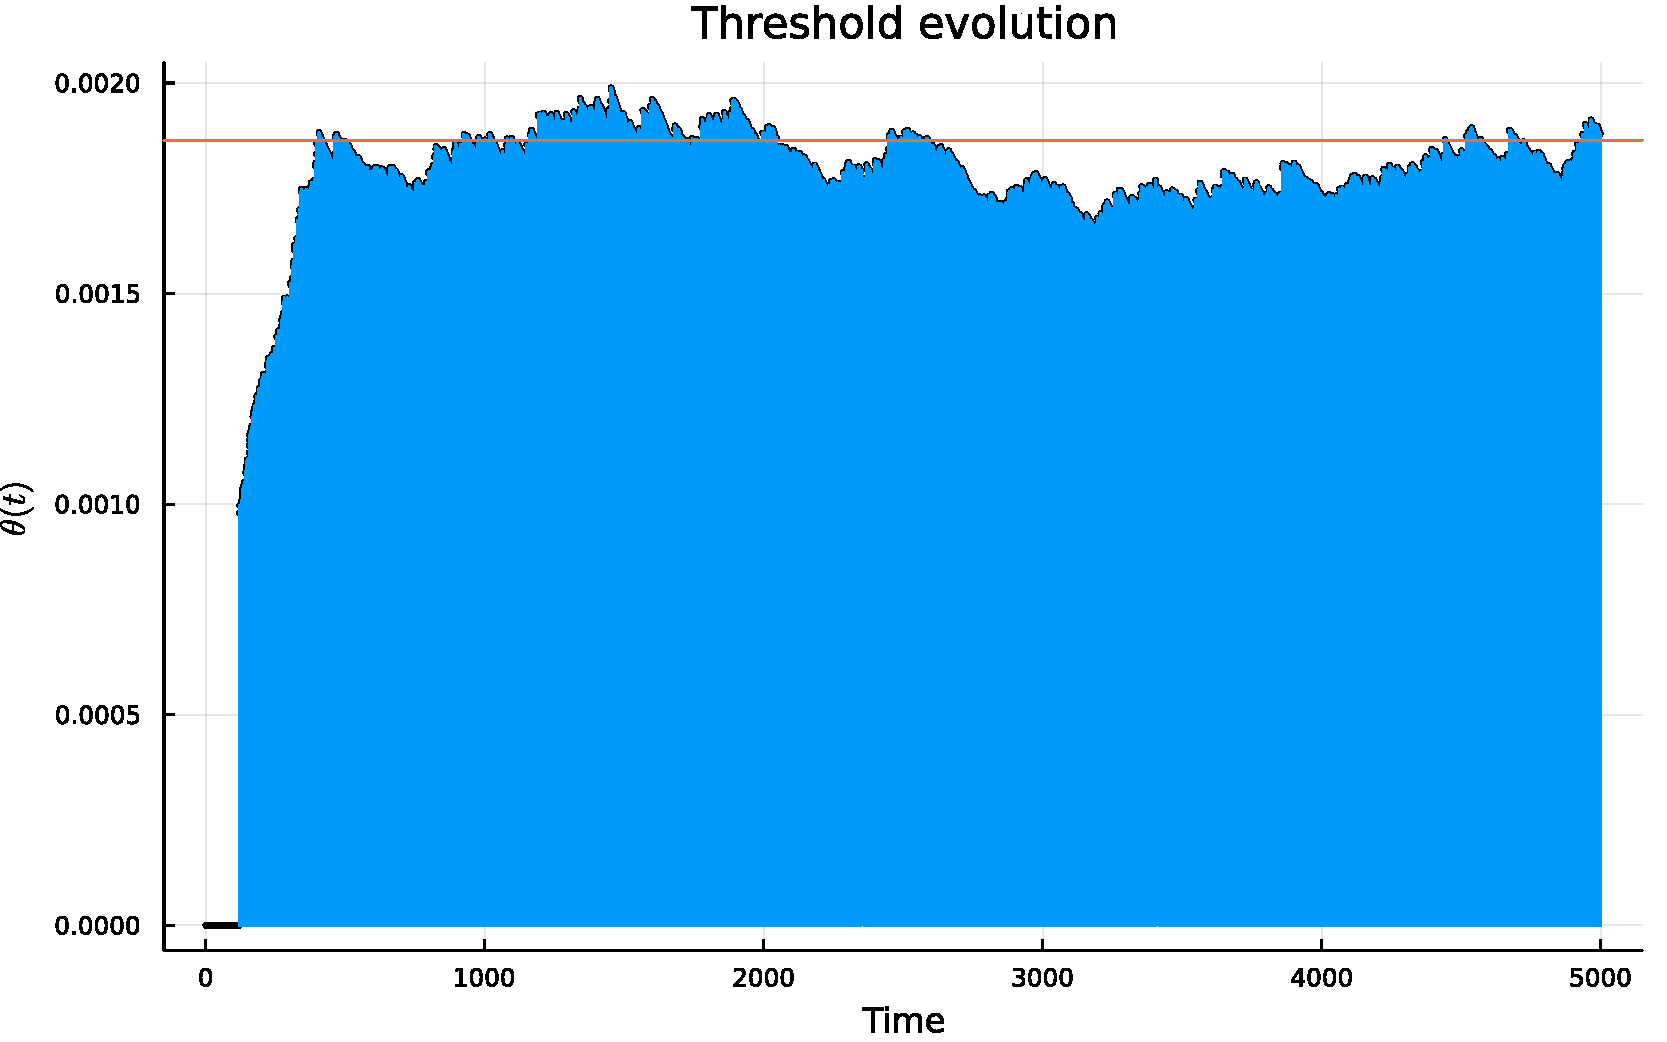
\includegraphics[width=0.65\textwidth]{figuras/simulation_example.pdf}

		{\footnotesize $M=1000, C=100$. Pareto $\alpha=2$ requests, Zipf $\beta=0.5$  popularities.}
	\end{center}
\end{frame}

\begin{frame}{Asymptotic miss probability}
	
	Moreover, we can calculate the asymptotic performance:

	\begin{theorem}
		Under all the above assumptions, the asymptotic \alert{miss rate} verifies:
		\begin{equation*}
			\lambda_{\text{miss},M} \to_M \int_0^\infty \lambda \tilde{G}_0\left(\frac{\theta^*}{\lambda}\right) \phi(d\lambda) = \E{\Lambda \tilde{G}_0\left(\frac{\theta^*}{\Lambda}\right)} 
		\end{equation*}
		where $\Lambda \sim \phi$, and $\tilde{G}_0$ is the distribution of the hazard-rate prior to an arrival:
		\begin{equation*}
			\tilde{G}_0(x) = \int_0^\infty \ind{\{\eta_0(t)\leqslant x\}} F_0(dt).
		\end{equation*}
	\end{theorem}
\end{frame}

\section{Connection with timer-based policies}

\begin{frame}{Populating a cache: timer based policies}
	
	\alert{Timer based (TTL) policies:}\vfill
	
	\begin{myitem}[1em]
		\item Upon request arrival for item $i$, check for presence.
		\item If new, store item and start a \alert{timer} $T_i$ to evict.
		\item If present, reset timer to $T_i$.
		\item Keep timers $T_i$ such that \alert{average} cache occupation is $C$.
	\end{myitem}
	
	\vspace{1.5em}
	
	\centering
	\resizebox{\textwidth}{!}{
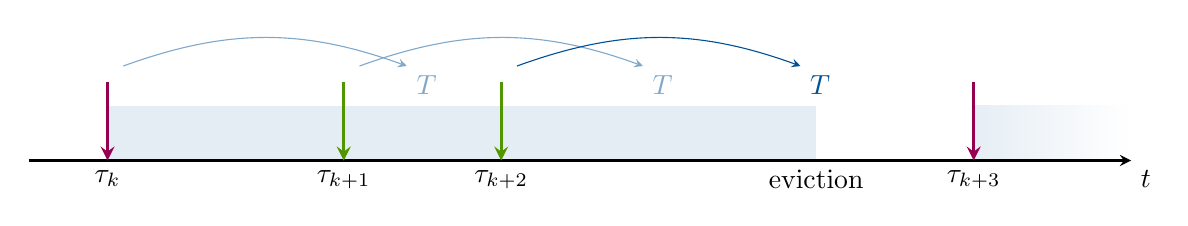
\begin{tikzpicture}
		\draw[white,fill=azulcito!10!white] (1,.7) rectangle (10,0);
		\shade[left color=azulcito!10!white, right color=white] (12,.7) rectangle (14,0);
	   
		\draw[->,thick] (0,0) -- (14,0);
		 \node[below right] at (14,0) {$t$};
		 
	   %  \draw[thick] (3,.1) -- (3,-.1);
	   %  \node[below left] at (3,0) {{\footnotesize $0$}};
	   
		 \draw[->,very thick, rojito] (1,1) -- (1,0);
		 \draw [->,azulcito!50!white] (1.2,1.2) to [out=20,in=160] (4.8,1.2) node [below right] {$T$};
		 \draw[->,very thick, verdecito] (4,1) -- (4,0);
		 \draw [->,azulcito!50!white] (4.2,1.2) to [out=20,in=160] (7.8,1.2) node [below right] {$T$};
		 \draw[->,very thick, verdecito] (6,1) -- (6,0);
		 \draw [->,azulcito] (6.2,1.2) to [out=20,in=160] (9.8,1.2) node [below right] {$T$};
		 \draw[->,very thick, rojito] (12,1) -- (12,0);
	   
		 \node[below] at (1,0) {$\tau_k$};
		 \node[below] at (4,0) {$\tau_{k+1}$};
		 \node[below] at (6,0) {$\tau_{k+2}$};
		 \node[below] at (12,0) {$\tau_{k+3}$};
		 \node[below] at (10,0) {\alert{eviction}};
		 
		 
\end{tikzpicture}
}
\end{frame}

\begin{frame}{Choosing the optimal timers}

	Requests come from independent sources with intensities $\lambda_i$ and inter-arrival distribution $F_i$:

	\vfill

	\begin{problem}[Optimal TTL policy]
		Choose timers $T_i\geqslant 0$ such that:
		\begin{equation*}
			\max_{T_i\geqslant 0} \sum_i \lambda_i F_i(T_i)
		\end{equation*}
		subject to:
		\begin{equation*}
			\sum_i \hat{F}_i(T_i) \leqslant C
		\end{equation*}
	\end{problem}

	\vfill
	\alert{Remark:} non-convex non-linear program. But it can be solved by a change of variables!!! [Ferragut et al. 2018].
\end{frame}

\begin{frame}{The optimal timers}

	\begin{theorem}
		For the following cases, the optimal timers are:

		\begin{itemize}
			\item Constant hazard rate (Poisson) or increasing hazard rate: keep the most popular objects ($T_i=\infty$ or $0$).
			
			\item Decreasing hazard rate:
			
			\begin{equation*}
				\eta_i (T_i^*) \geqslant \theta^*
			   \end{equation*}
			  for every stored content.
		\end{itemize}
	\end{theorem}
	\pause
	\vfill
\end{frame}

\begin{frame}{Why this happens?}
	
	So the optimal timer policy is a threshold policy?  %{\LARGE{\emoji{thinking}}}

	\pause 
	\begin{center}
		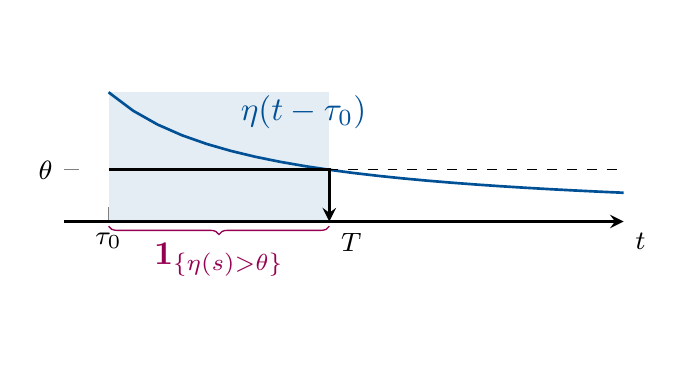
\begin{tikzpicture}[scale=1.2]
			\begin{axis}[xlabel=$t$,
				ymin = -2,
				ymax = 3,
				xmin = -.3,
				xmax = 3.5,
				xlabel style = {at={(axis cs:3.5,0)},anchor=north west},
				y axis line style={draw=none},
				x axis line style={->, thick},
				ytick=\empty,
				axis x line*=middle,
				axis y line*=left,
				width=7.5cm,
				height=5cm,
				xtick={0,4},
				ytick={.8},
				xticklabels={$\tau_0$,$\tau_1$},
				yticklabels={$\theta$},
				]
				\addplot[domain=0:4,thick,azulcito] {2/(1+x)} node[midway, yshift=10, xshift=3,anchor=south east]{$\eta(t-\tau_0)$};
				\addplot[domain=0:4,dashed] {0.8};
				\fill[color=azulcito, opacity=0.1] (0,0) rectangle (1.5,2);
				\draw [rojito,decoration={mirror,brace,raise=0.05cm},decorate] (axis cs:0,0) -- (axis cs:1.5,0) node [pos=0.5,anchor=north,yshift=-0.1cm] {$\mathbf{1}_{\{\eta(s)>\theta\}}$};
				\node[below right] at (1.5,0) {\footnotesize $T$};
				\draw[stealth-, thick] (1.5,0) -- (1.5,0.8) -- (0,0.8);
			\end{axis}
		\end{tikzpicture}
		\end{center}

\end{frame}
\begin{frame}{Asymptotic optimality}

	\begin{theorem}[F', Carrasco, Paganini]

		In the scaling regime considered earlier, for renewal processes with DHR, the optimal TTL policy is also asymptotically optimal within the class of causal policies.
	\end{theorem}
	\vfill
	\alert{Idea:} prove that the thresholds are the same in the limit.

	\pause
	But what about \alert{increasing hazard rates}?
\end{frame}

\begin{frame}{Back to increasing hazard rates...}

	\begin{myitem}[2em]
	\item Recall the increasing hazard rate behavior:
	
	\bigskip

	\begin{center}
	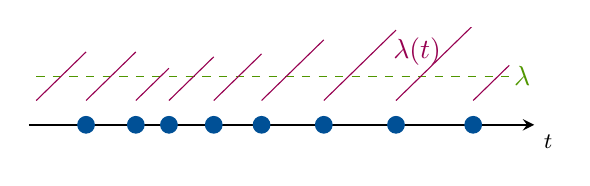
\begin{tikzpicture}
		\begin{axis}[xlabel=$t$,
			ymin = -.3,
			ymax = 2,
			xmin = -.3,
			xmax=20,
			xlabel style = {at={(axis cs:20,0)},anchor=north west},
			y axis line style={draw=none},
			x axis line style={->, thick},
			ticks=none,
			axis x line*=middle,
			width=8cm,
			height=3cm,
			]
			\addplot[verdecito,domain=0:19, dashed] {1};
			\addplot[rojito,domain=0:2] {0.5+0.5*x};
			\addplot[rojito,domain=2:4] {0.5+0.5*(x-2};
			\addplot[rojito,domain=4:5.33] {0.5+0.5*(x-4};
			\addplot[rojito,domain=5.33:7.13] {0.5+0.5*(x-5.33};
			\addplot[rojito,domain=7.13:9.05] {0.5+0.5*(x-7.13};
			\addplot[rojito,domain=9.05:11.55] {0.5+0.5*(x-9.05};
			\addplot[rojito,domain=11.55:14.45] {0.5+0.5*(x-11.55};
			\addplot[rojito,domain=14.45:17.55] {0.5+0.5*(x-14.45};
			\addplot[rojito,domain=17.55:19] {0.5+0.5*(x-17.55};
			\node[below, rojito] at (axis cs:15.3,2) {$\lambda(t)$};
			\node[right, verdecito] at (axis cs:18.8,1) {$\lambda$};

			\addplot+[azulcito, mark options={fill=azulcito, scale=1.5}, mark=*,only marks] coordinates {
				(2,0)
				(4,0)
				(5.33,0)
				(7.13,0)
				(9.05,0)
				(11.55,0)
				(14.45,0)
				(17.55,0)
			};
		\end{axis}
	\end{tikzpicture}
	\end{center}
	\item Once you have seen a request, it's less likely to see another one for a while.
	\end{myitem}

	\pause
	\vfill

	\begin{center}
		\alert{What is the timer based equivalent of this case?}
	\end{center}

\end{frame}

\begin{frame}{Timer based pre-fetching policies}


\begin{block}{Key insight}
The question now is not \alert{how long we should remember something}, but instead \alert{how long we should forget about it}!
\end{block}

\vfill

\pause

\alert{Timer based pre-fetching policy:}

\vfill

\resizebox{\textwidth}{!}{
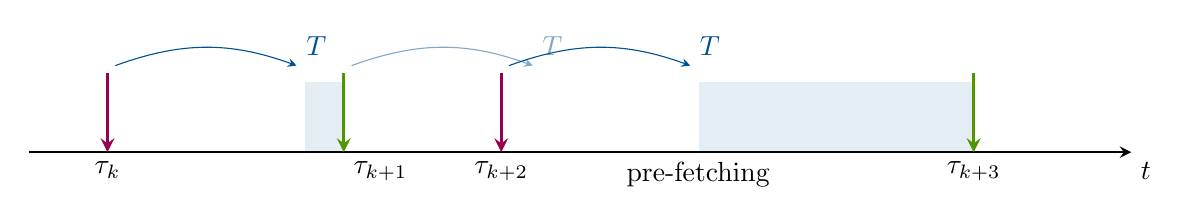
\begin{tikzpicture}
		\draw[white,fill=azulcito!10!white] (3.5,.9) rectangle (4,0);
		\draw[white,fill=azulcito!10!white] (8.5,.9) rectangle (12,0);
		
		\draw[->,thick] (0,0) -- (14,0);
		 \node[below right] at (14,0) {$t$};
		 
	   %  \draw[thick] (3,.1) -- (3,-.1);
	   %  \node[below left] at (3,0) {{\footnotesize $0$}};
	   
		 \draw[->,very thick, rojito] (1,1) -- (1,0);
		 \draw [->,azulcito] (1.1,1.1) to [out=20,in=160] (3.4,1.1) node [above right] {$T$};
		 \draw[->,very thick, verdecito] (4,1) -- (4,0);
		 \draw [->,azulcito!50!white] (4.1,1.1) to [out=20,in=160] (6.4,1.1) node [above right] {$T$};
		 \draw[->,very thick, rojito] (6,1) -- (6,0);
		 \draw [->,azulcito] (6.1,1.1) to [out=20,in=160] (8.4,1.1) node [above right] {$T$};
		 \draw[->,very thick, verdecito] (12,1) -- (12,0);
	   
		 \node[below] at (1,0) {$\tau_k$};
		 \node[below right] at (4,0) {$\tau_{k+1}$};
		 \node[below] at (6,0) {$\tau_{k+2}$};
		 \node[below] at (12,0) {$\tau_{k+3}$};
		 \node[below] at (8.5,0) {\alert{pre-fetching}};
		 
\end{tikzpicture}
}

\end{frame}

% \begin{frame}{Timer based pre-fetching}
	
% 	Consider a single item with a timer $T$ and its request process:

% 	\bigskip

% 	\begin{columns}[T]
% 		\begin{column}{.5\textwidth}
% 		\textbf{Hit probability:} \alert{next} arrival occurs \alert{after} timer expires.

% 		\bigskip
		
% 		\begin{center}

% 		\begin{tikzpicture}[scale=1]
% 			\draw[white,fill=azulcito!10!white] (3.5,.9) rectangle (4,0);
% 		  \draw[->,thick] (0,0) -- (6,0);
% 		  \node[below right] at (6,0) {\footnotesize $t$};
		
% 		  \draw[->,very thick, rojito] (1,1) -- (1,0);
% 		  \draw [->,thick,azulcito] (1.1,1.1) to [out=20,in=160] (3.4,1.1) node [above right] {$T$};
% 		  \draw [->,thick,black] (1.1,.2) -- (3.9,.2) node [above, midway] {$X \sim F(x)$};
% 		  \draw[->,very thick, verdecito] (4,1) -- (4,0);
% 		  \node[azulcito,below] at (3,-.5) {Hit probability $=1-F(T)$};
% 		  \end{tikzpicture}
% 		  \end{center}
		
% 		\end{column}
		
% 		\begin{column}{0.5\textwidth}

% 		\textbf{Occupation probability:} probability that timer \alert{has} expired by $0$ since last arrival.

% 		\begin{center}

% 		 \bigskip

% 		 \begin{tikzpicture}
% 		 \draw[white,fill=azulcito!10!white] (3.5,0.9) rectangle (5,0); 
% 		 \shade[left color=azulcito!10!white, right color=white] (5,.9) rectangle (6,0);
% 		  \draw[->,thick] (0,0) -- (6,0);
% 		  \node[below right] at (6,0) {\footnotesize $t$};
		  
% 		  \draw[thick] (4.5,.1) -- (4.5,-.1);
% 		  \node[below right] at (4.5,0) {{\footnotesize $0$}};
		
% 		  \draw[->,very thick, rojito] (1,1) -- (1,0);
% 		  \draw [->,thick,azulcito] (1.1,1.1) to [out=20,in=160] (3.4,1.1) node [above right] {$T$};		 % \draw[->,very thick, rojito!20!white] (5.75,1) -- (5.75,0);
% 		  \draw [<-,thick, black] (1.1,.2) -- (4.5,.2) node [above, midway] {$\hat{X}\sim\hat{F}(x)$};
		  
% 		  \node[azulcito,below] at (3,-.5) {Avg. occupation $= 1-\hat{F}(T)$};
% 		\end{tikzpicture}
% 		\end{center}
		
% 		\end{column}
% 		\end{columns}
% \end{frame}

\begin{frame}{Choosing the optimal timers}

	Requests come from independent sources with intensities $\lambda_i$ and inter-arrival distribution $F_i$:

	\vfill

	\only<1>{
	\begin{problem}[Optimal pre-fetching policy]
		Choose timers $T_i\geqslant 0$ such that:
		\begin{equation*}
			\max_{T_i\geqslant 0} \sum_i \lambda_i (1-F_i(T_i))
		\end{equation*}
		subject to:
		\begin{equation*}
			\sum_i (1-\hat{F}_i(T_i)) \leqslant C
		\end{equation*}
	\end{problem}
	}
	\only<2->{
		\begin{problem}[Optimal pre-fetching policy]
			Choose timers $T_i\geqslant 0$ such that:
			\begin{equation*}
				\min_{T_i\geqslant 0} \sum_i \lambda_i F_i(T_i)
			\end{equation*}
			subject to:
			\begin{equation*}
				\sum_i \hat{F}_i(T_i) \geqslant N-C
			\end{equation*}
		\end{problem}		
	}
	\vfill
	\pause
	\alert{Remark:} we can use the same change of variables again!
\end{frame}

\begin{frame}{Pre-fetching for increasing hazard rates}

	\begin{block}{Optimal pre-fetching policy, IHR, [F',Carrasco, Paganini].}
		The optimal timer based pre-fetching policy for IHR is such that:
	   \begin{equation*}
		\eta_i (T_i^*) \geqslant \theta^*
	   \end{equation*}
	  for every stored content.
	   \end{block}
	  \vfill
	
	
	  \alert{Remark:} Again we have to equalize hazard-rates. The policy is a threshold policy.

\end{frame}

\begin{frame}{Asymptotic optimality}

	\begin{theorem}[F', Carrasco, Paganini]

		In the scaling regime considered earlier, for renewal processes with IHR, the \alert{timer based pre-fetching policy} is asymptotically optimal.
	\end{theorem}
	\vfill
	\alert{Idea:} as before, prove that the thresholds are the same in the limit.

\end{frame}

\section{Conclusions}

\begin{frame}{Final remarks}
	
	\begin{myitem}[2em]
		\item The main result characterizes the optimal policy completely in the large-scale scenario.
		
		\item For particular distributions of interest (e.g. Pareto requests, Zipf popularities) the threshold can be computed explicitly.
		
		\item Once the threshold is computed, we can compute the asymptotic hit probability.
		
		\item Therefore, we have a computable absolute performance bound in the limit.
		\pause
		\item There is much more to do!
		
	\end{myitem}
\end{frame}


\begin{frame}[plain]
	\vfill
	{\Huge \alert{Merci beaucoup!}}
	\vfill
	Andres Ferragut

	\href{mailto://ferragut@ort.edu.uy}{\alert{\texttt{ferragut@ort.edu.uy}}}
	
	\href{http://aferragu.github.io}{\alert{\texttt{aferragu.github.io}}}
\end{frame}

\end{document}
